\subsection{Практическая часть}
\subsubsection{Настройка доменной системы}
В практике используются виртуальные машины Windows Server 2003 и Windows 10, 
заранее присоединим компьютер к домену, и далее создадим подразделения для
нашей организации соответственно варианту.

Для нашей структуры создадим матрицу доступа субъектов к объектам.
\begin{figure}[H]
  \centering
  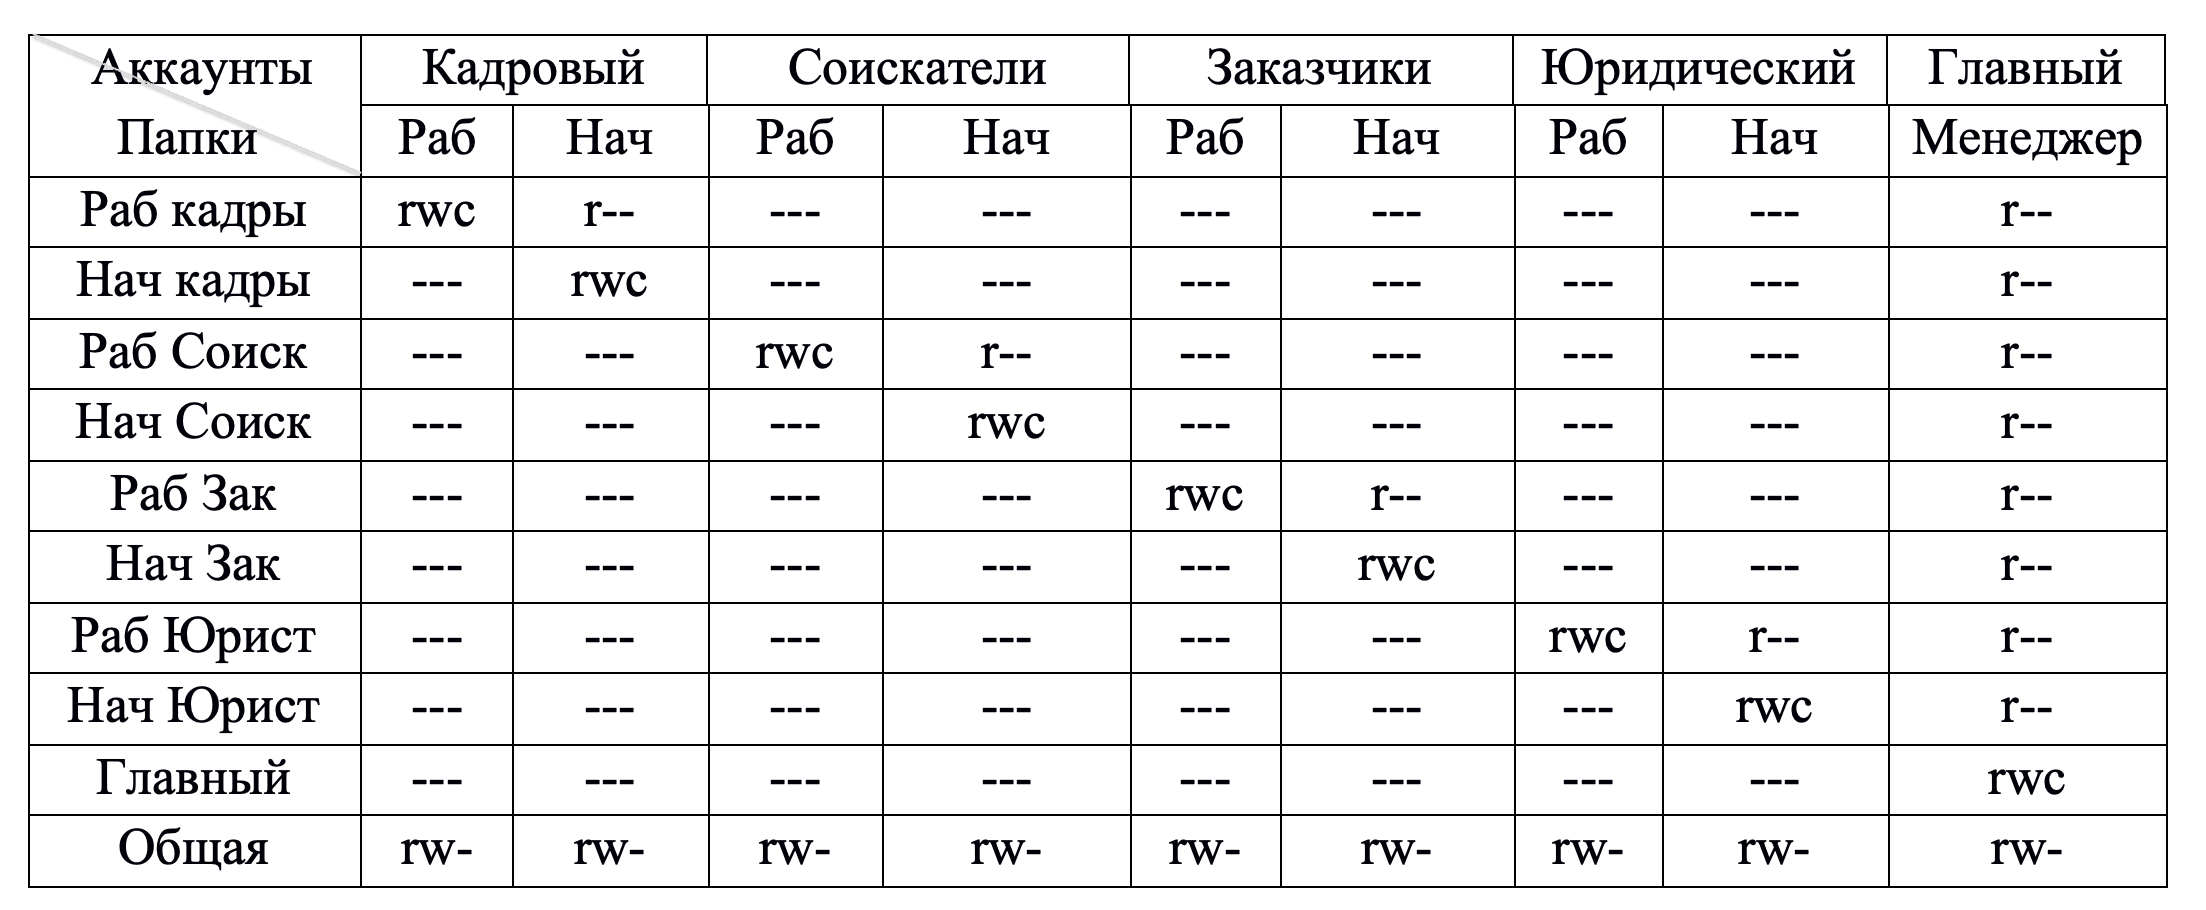
\includegraphics[width=1\textwidth]{pict/102}
  \caption{Матрица доступа, r - чтение, w - запись, c - изменение}
  \label{fig:101}
\end{figure}

\begin{figure}[H]
  \centering
  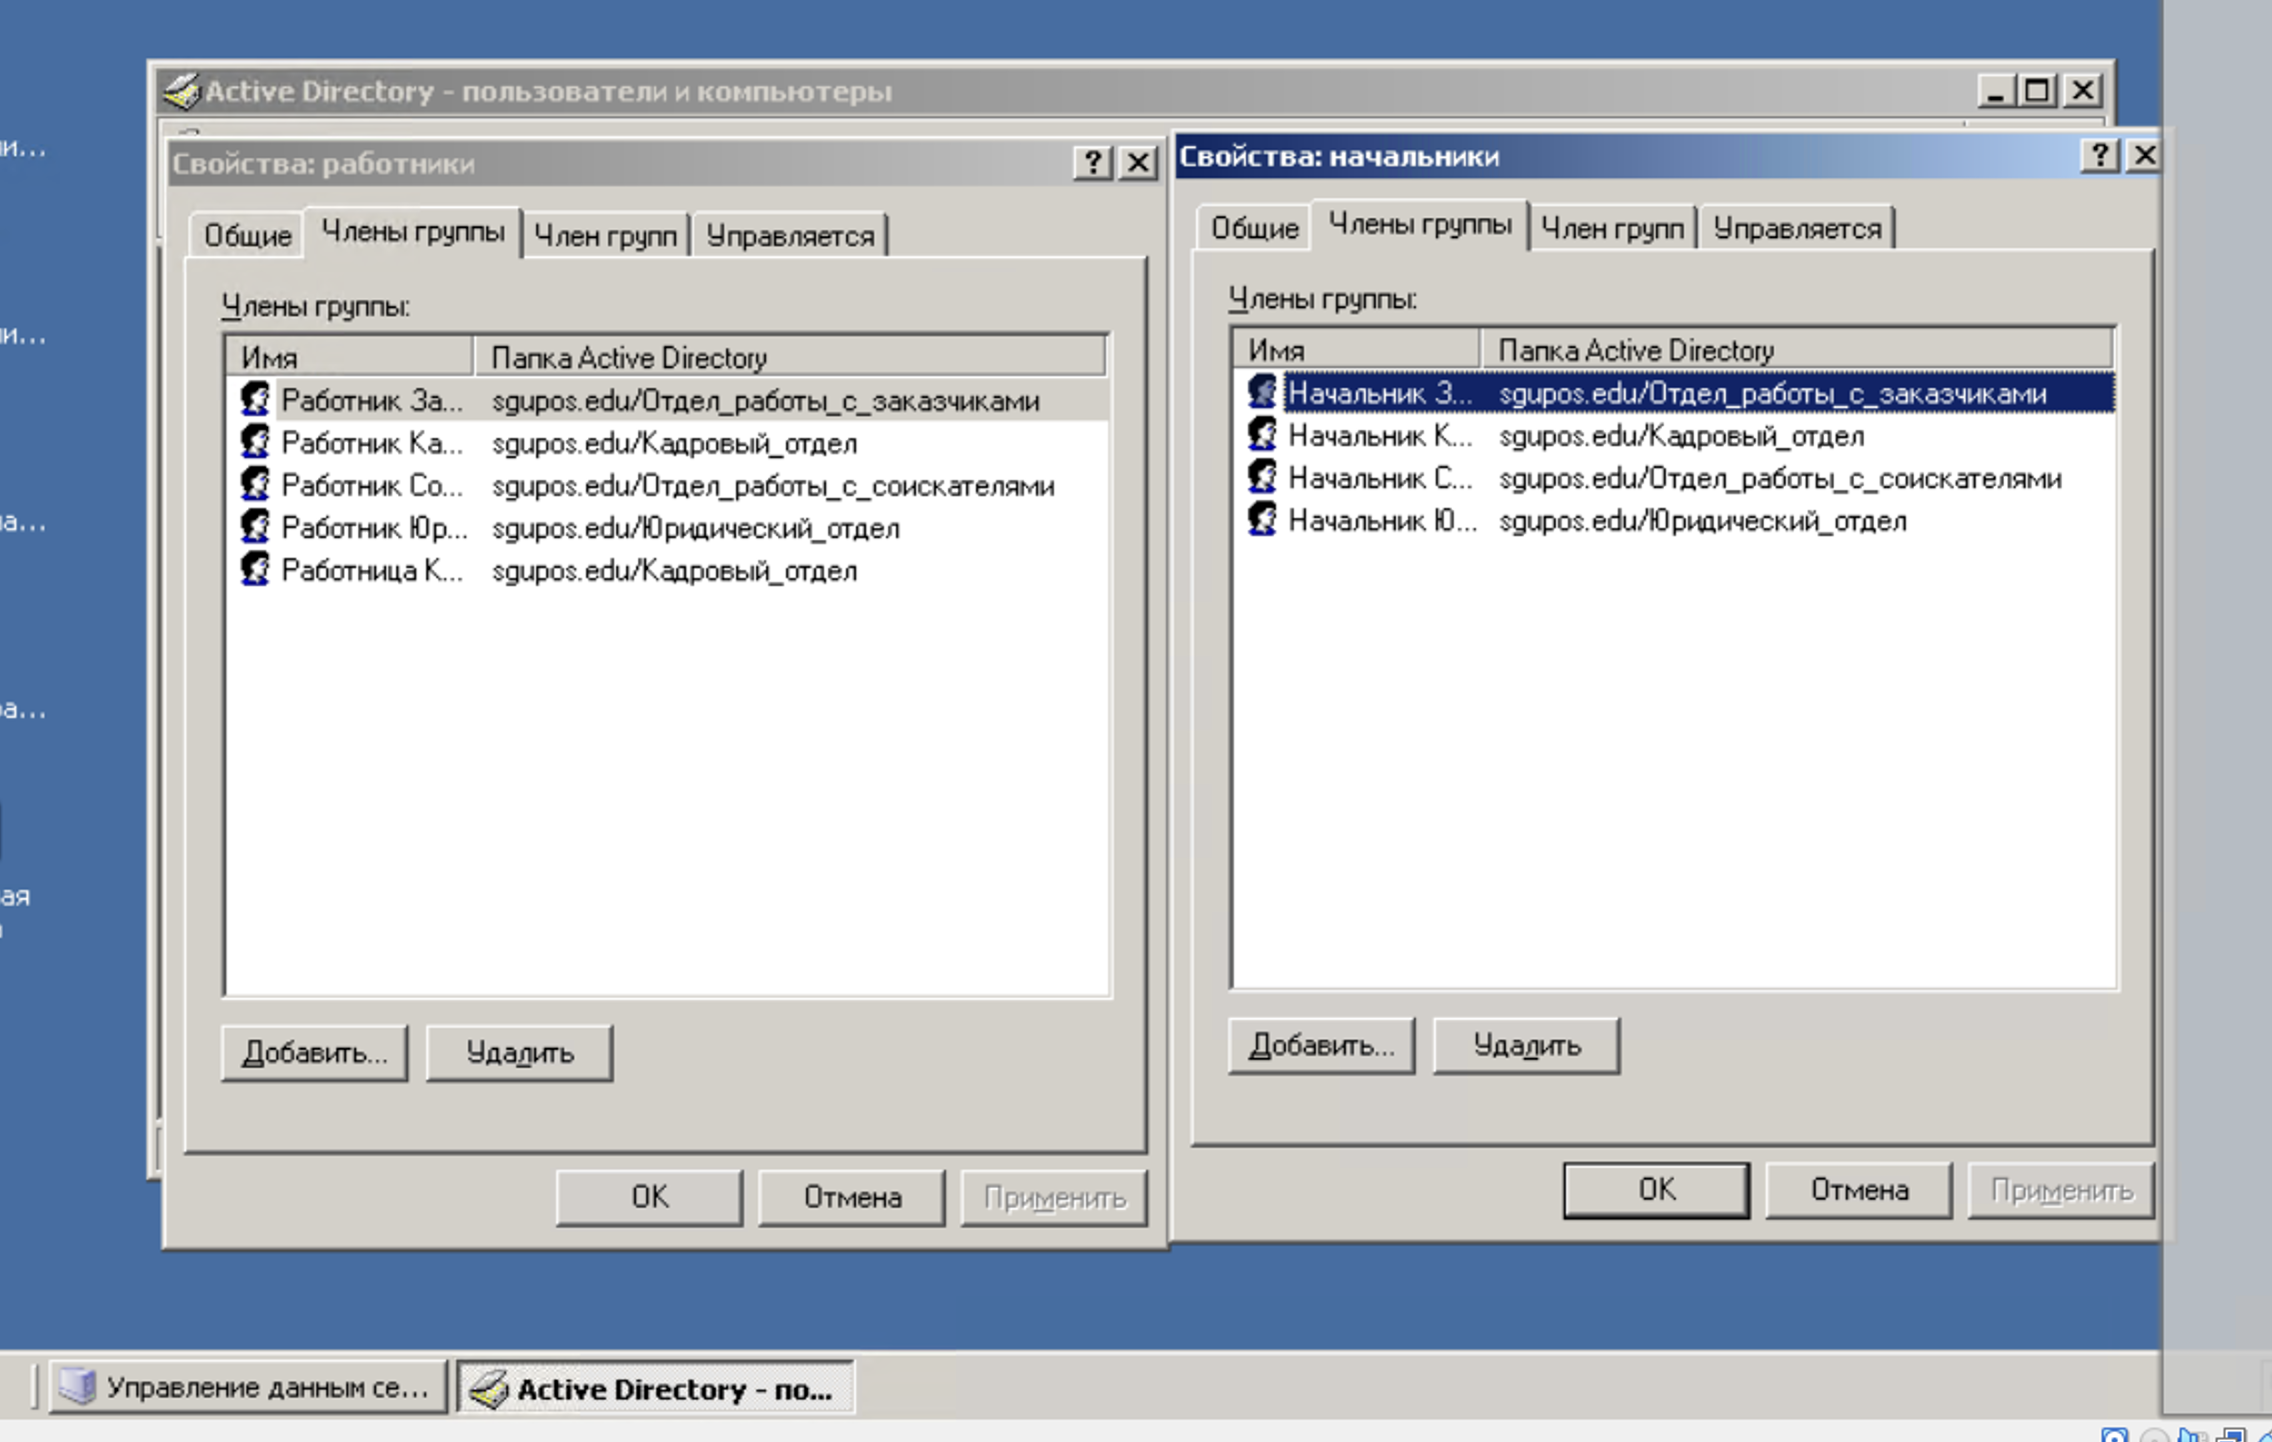
\includegraphics[width=1\textwidth]{pict/prac/54}
  \caption{}
\end{figure}

В домене создадим подразделения соответствующие варианту, а также на одном уровне с ними создадим 
главного пользователя.

\begin{figure}[H]
  \centering
  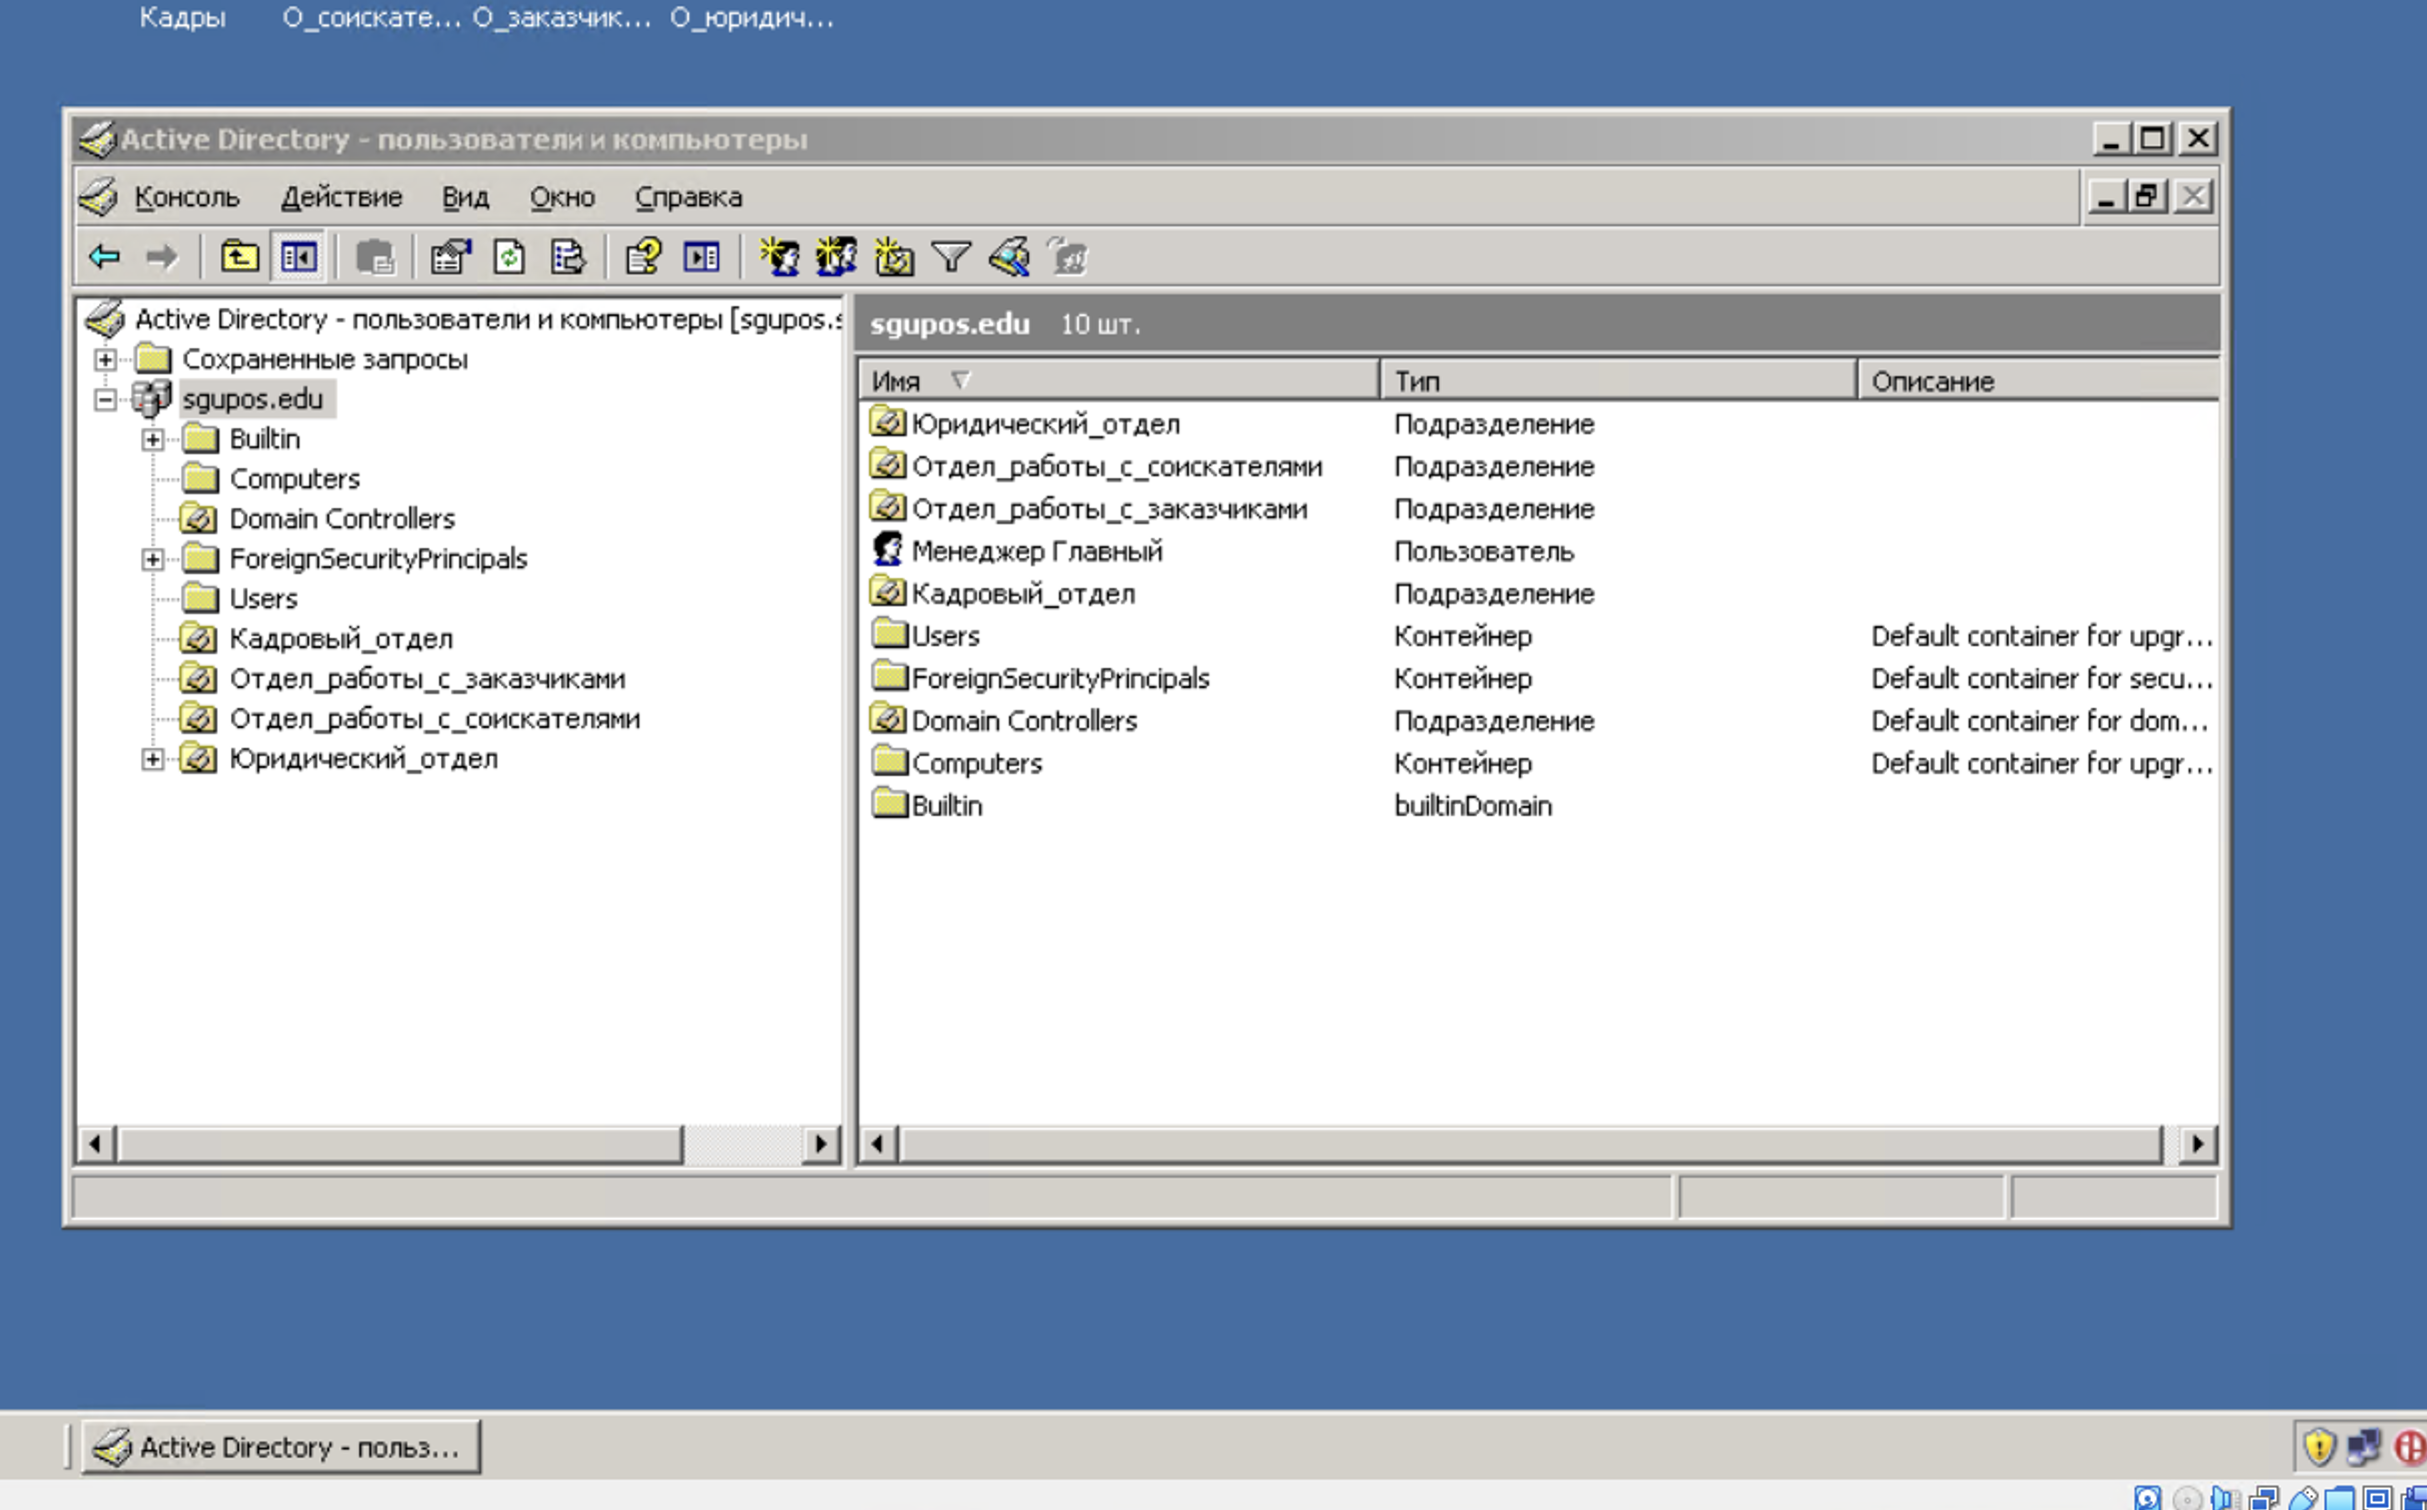
\includegraphics[width=1\textwidth]{pict/prac/3}
  \caption{Подразделения}
  \label{fig:11}
\end{figure}

Одним из требований к классу АС является установка для пользователя пароля длинной не менее 6 
цифро-буквенных символов, включим эту настройку.
\begin{figure}[H]
  \centering
  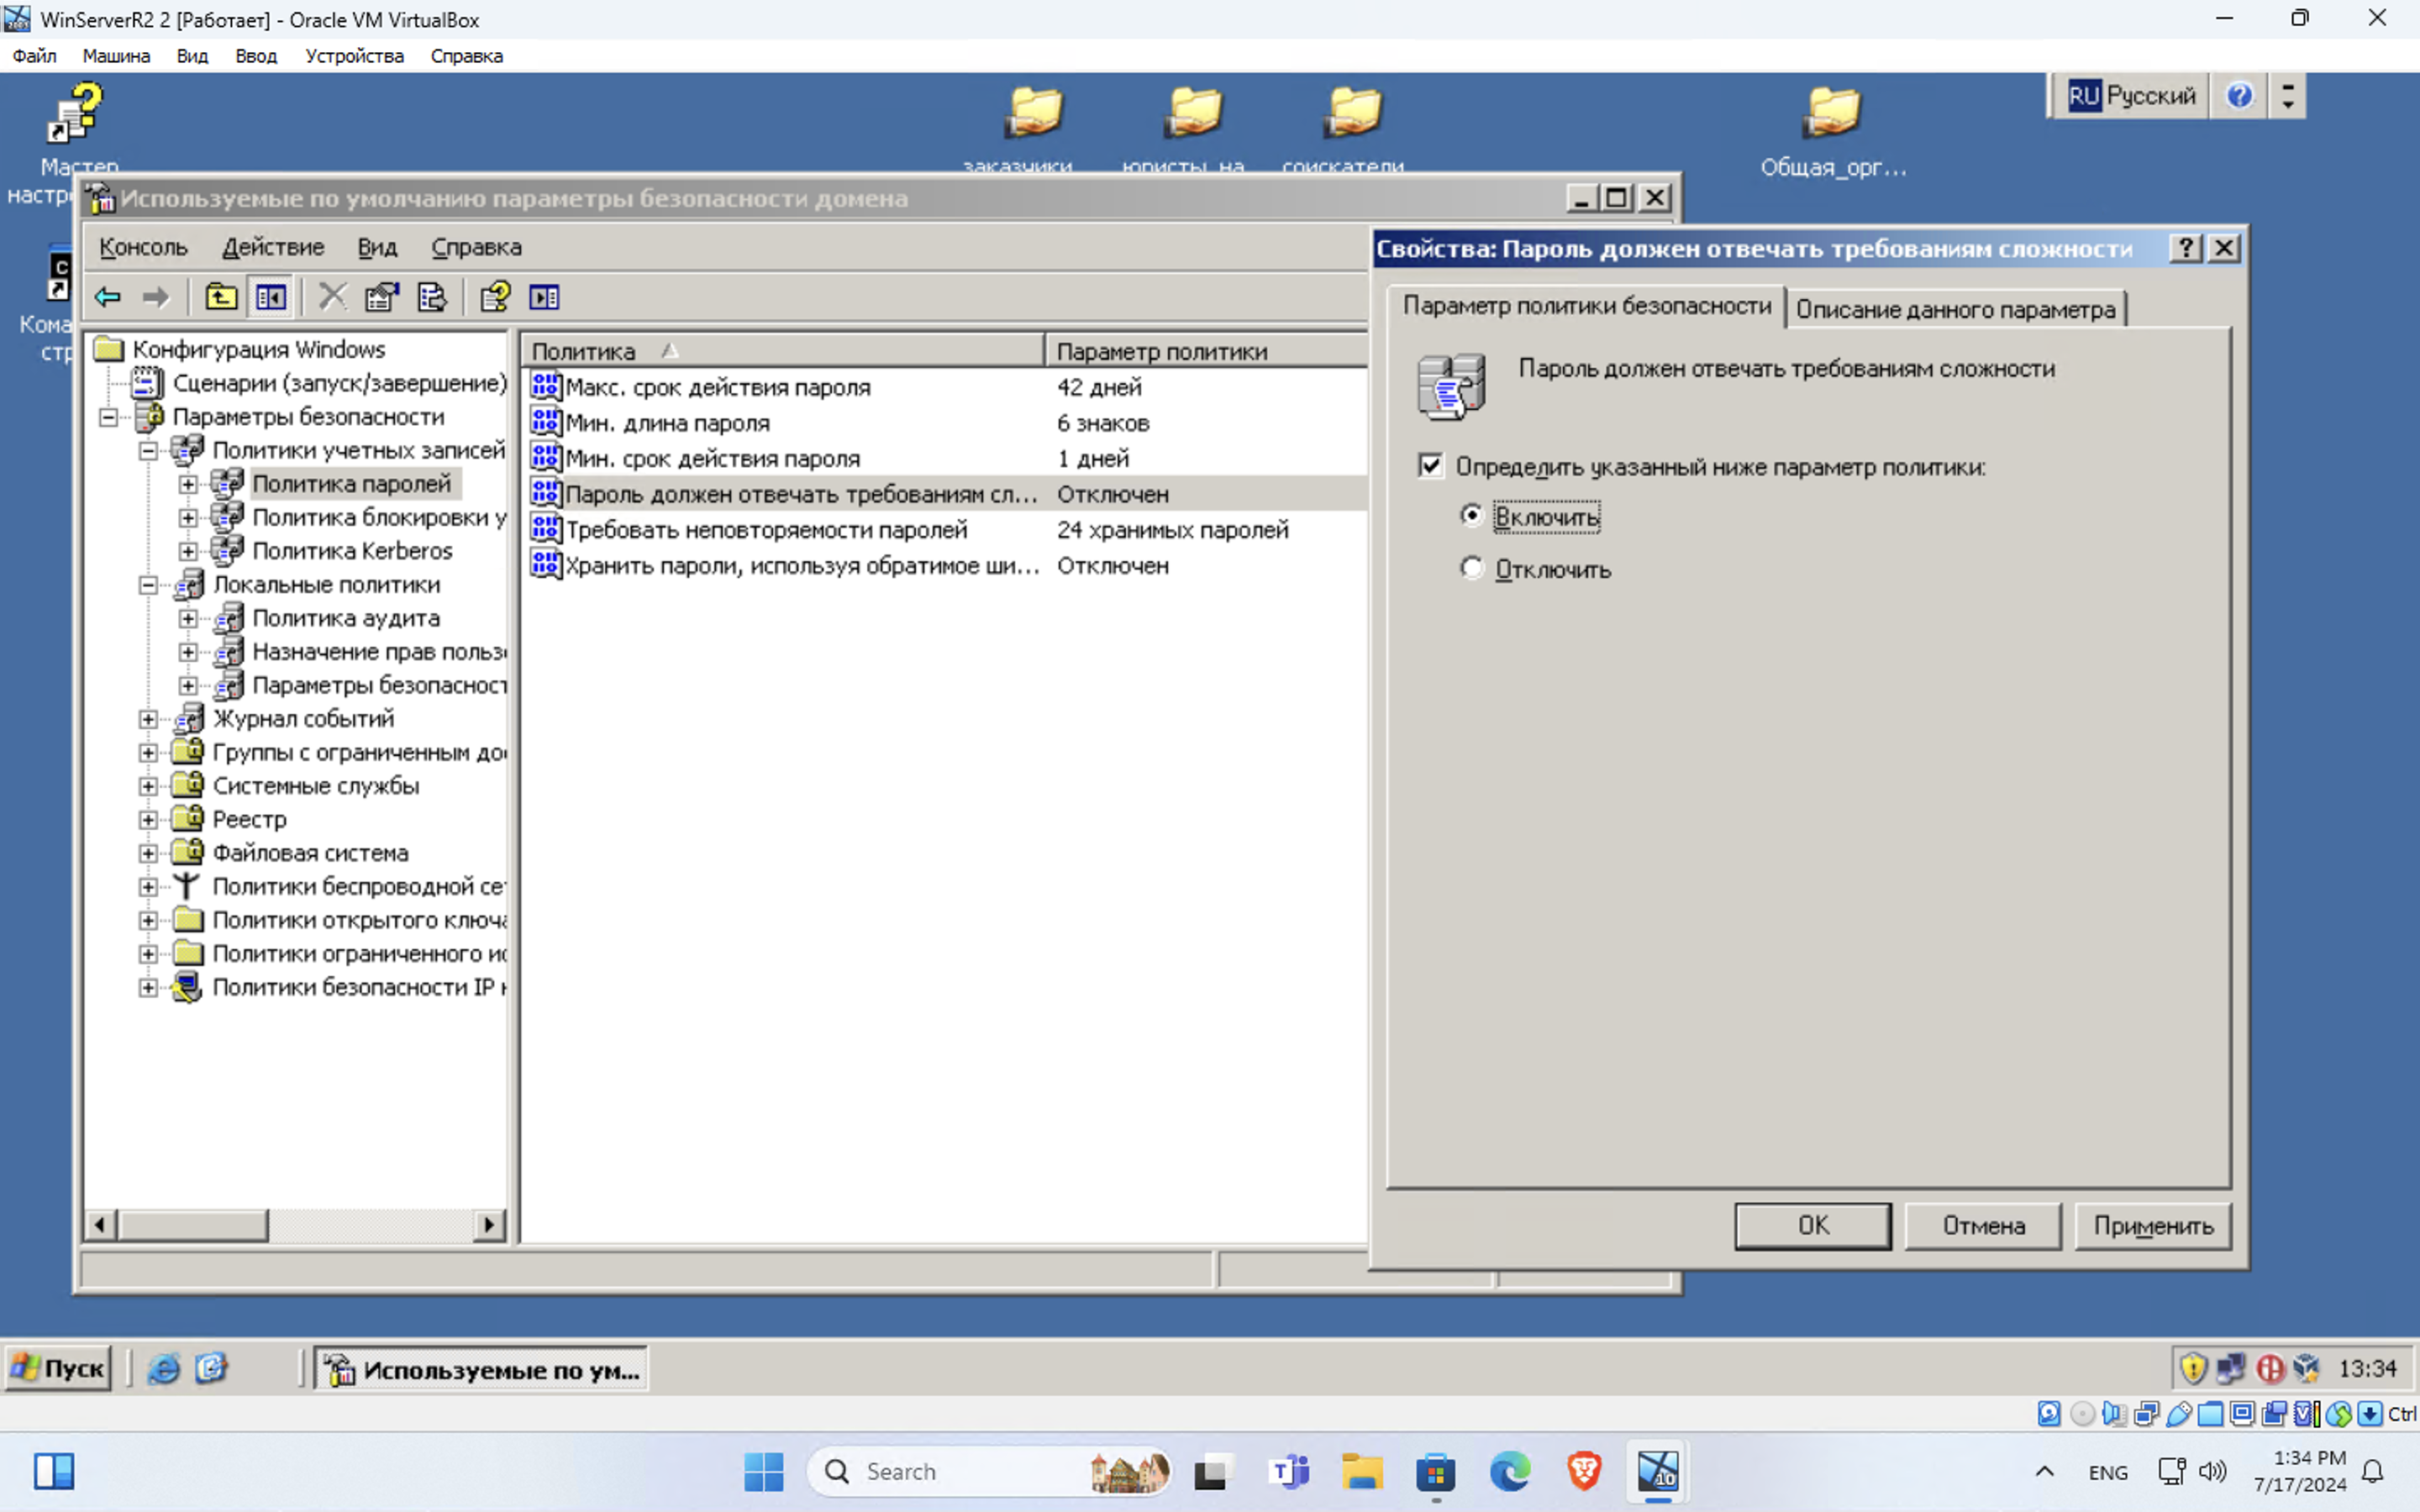
\includegraphics[width=1\textwidth]{pict/7}
  \caption{Парольная политика}
  \label{fig:19}
\end{figure}

Создадим пользователей в каждом подразделении.
\begin{figure}[H]
  \centering
  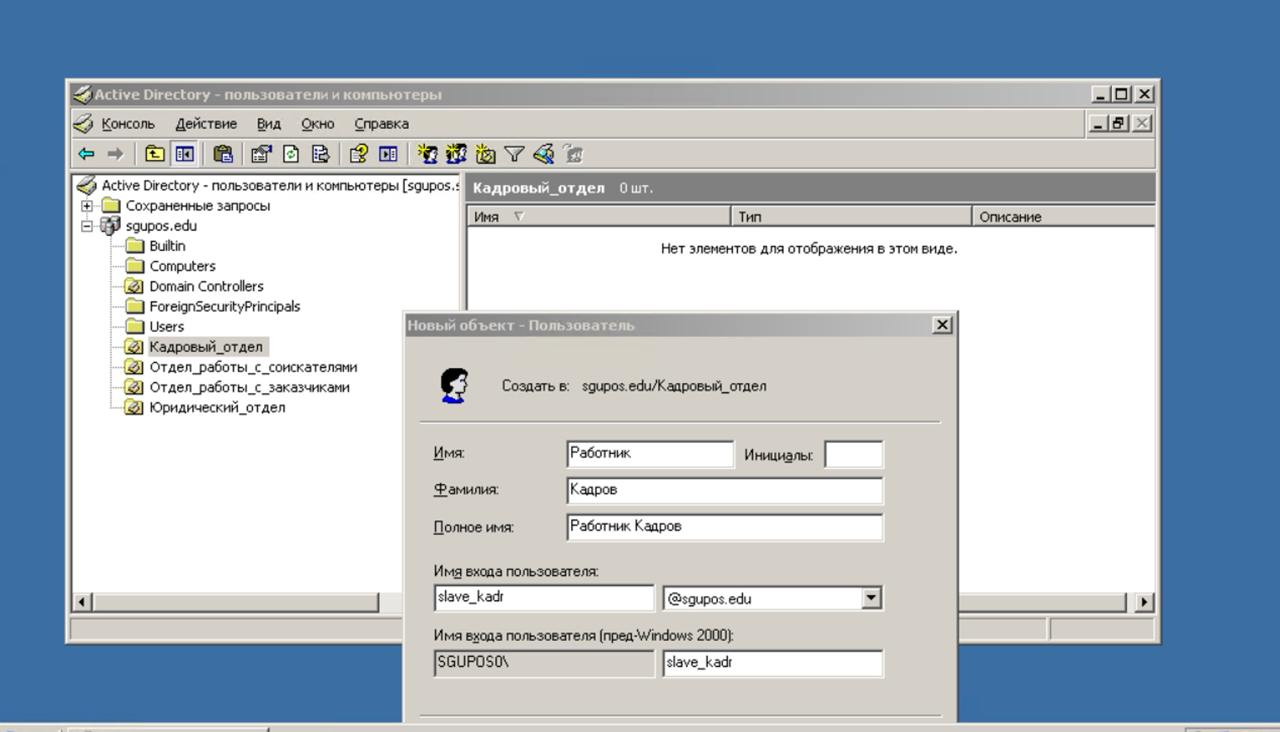
\includegraphics[width=1\textwidth]{pict/prac/1}
  \caption{Создание пользователя}
  \label{fig:12}
\end{figure}

\begin{figure}[H]
  \centering
  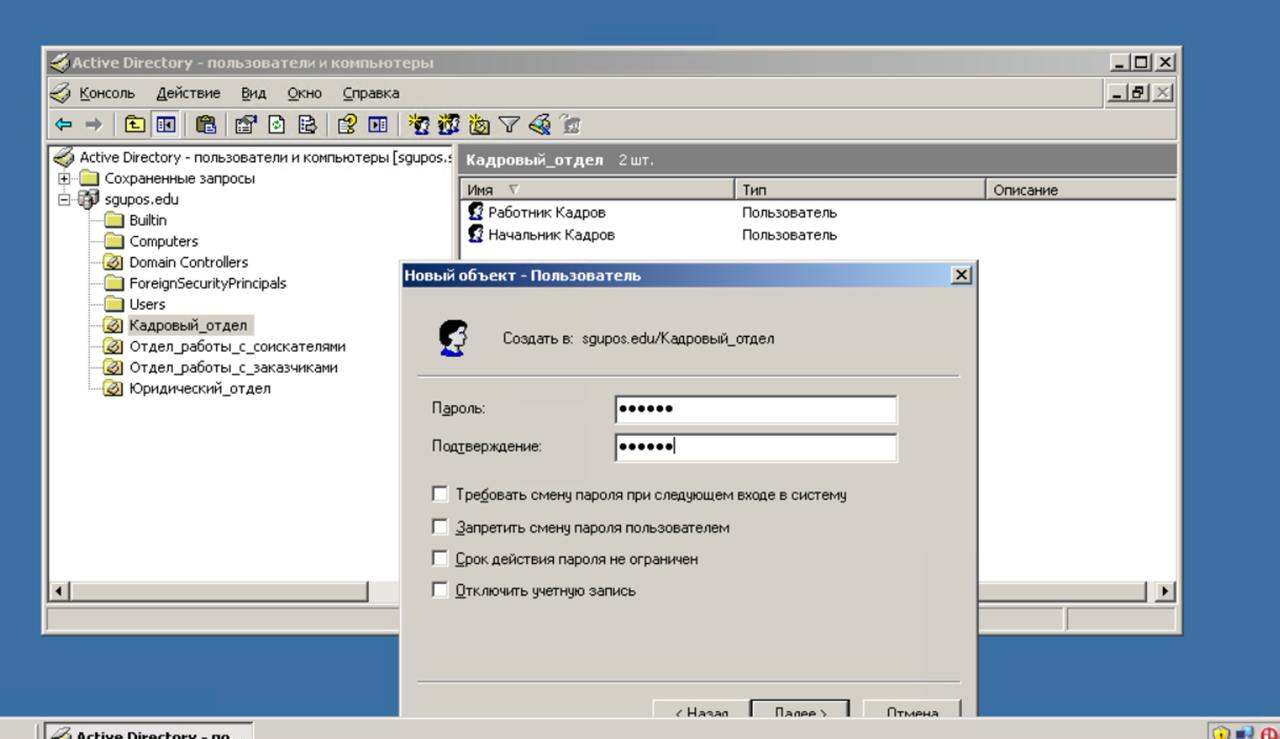
\includegraphics[width=1\textwidth]{pict/prac/2}
  \caption{Задание пароля пользователю}
  \label{fig:14}
\end{figure}

Проверим работу настройки сложности пароля, поменяем пользователю пароль.
\begin{figure}[H]
  \centering
  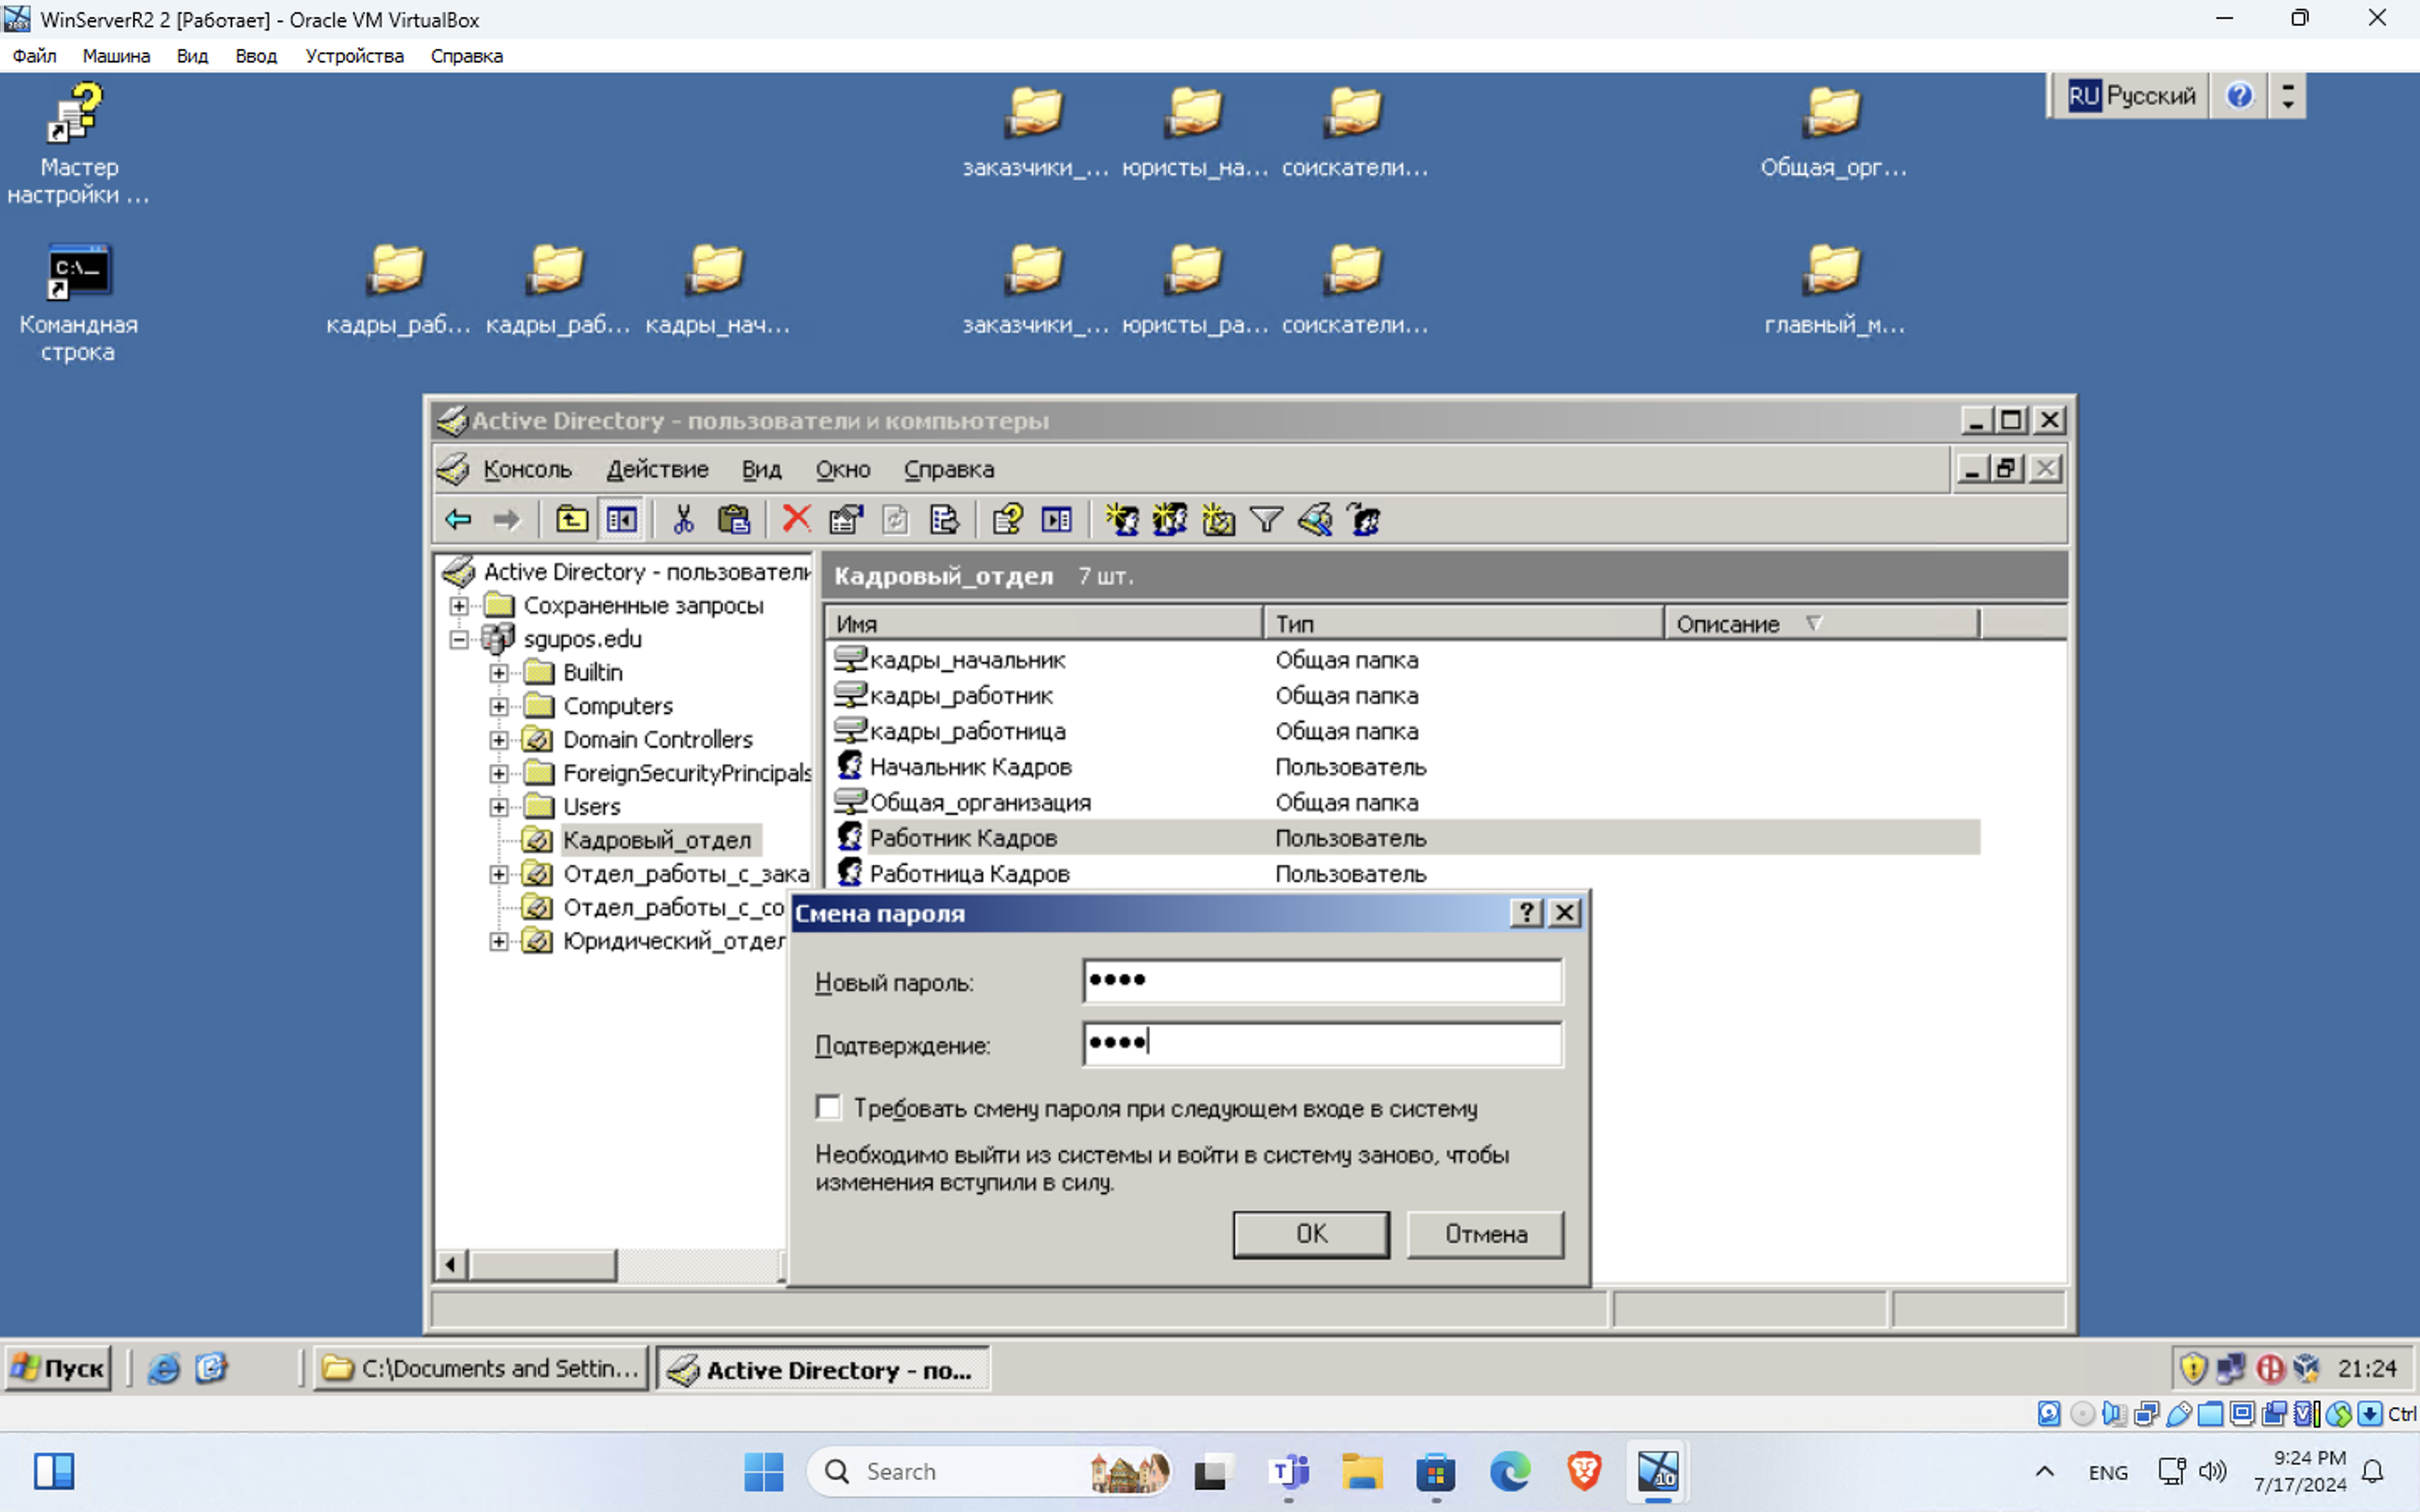
\includegraphics[width=1\textwidth]{pict/prac/50}
  \caption{Поменяем пароль на более короткий}
  \label{fig:50}
\end{figure}

\begin{figure}[H]
  \centering
  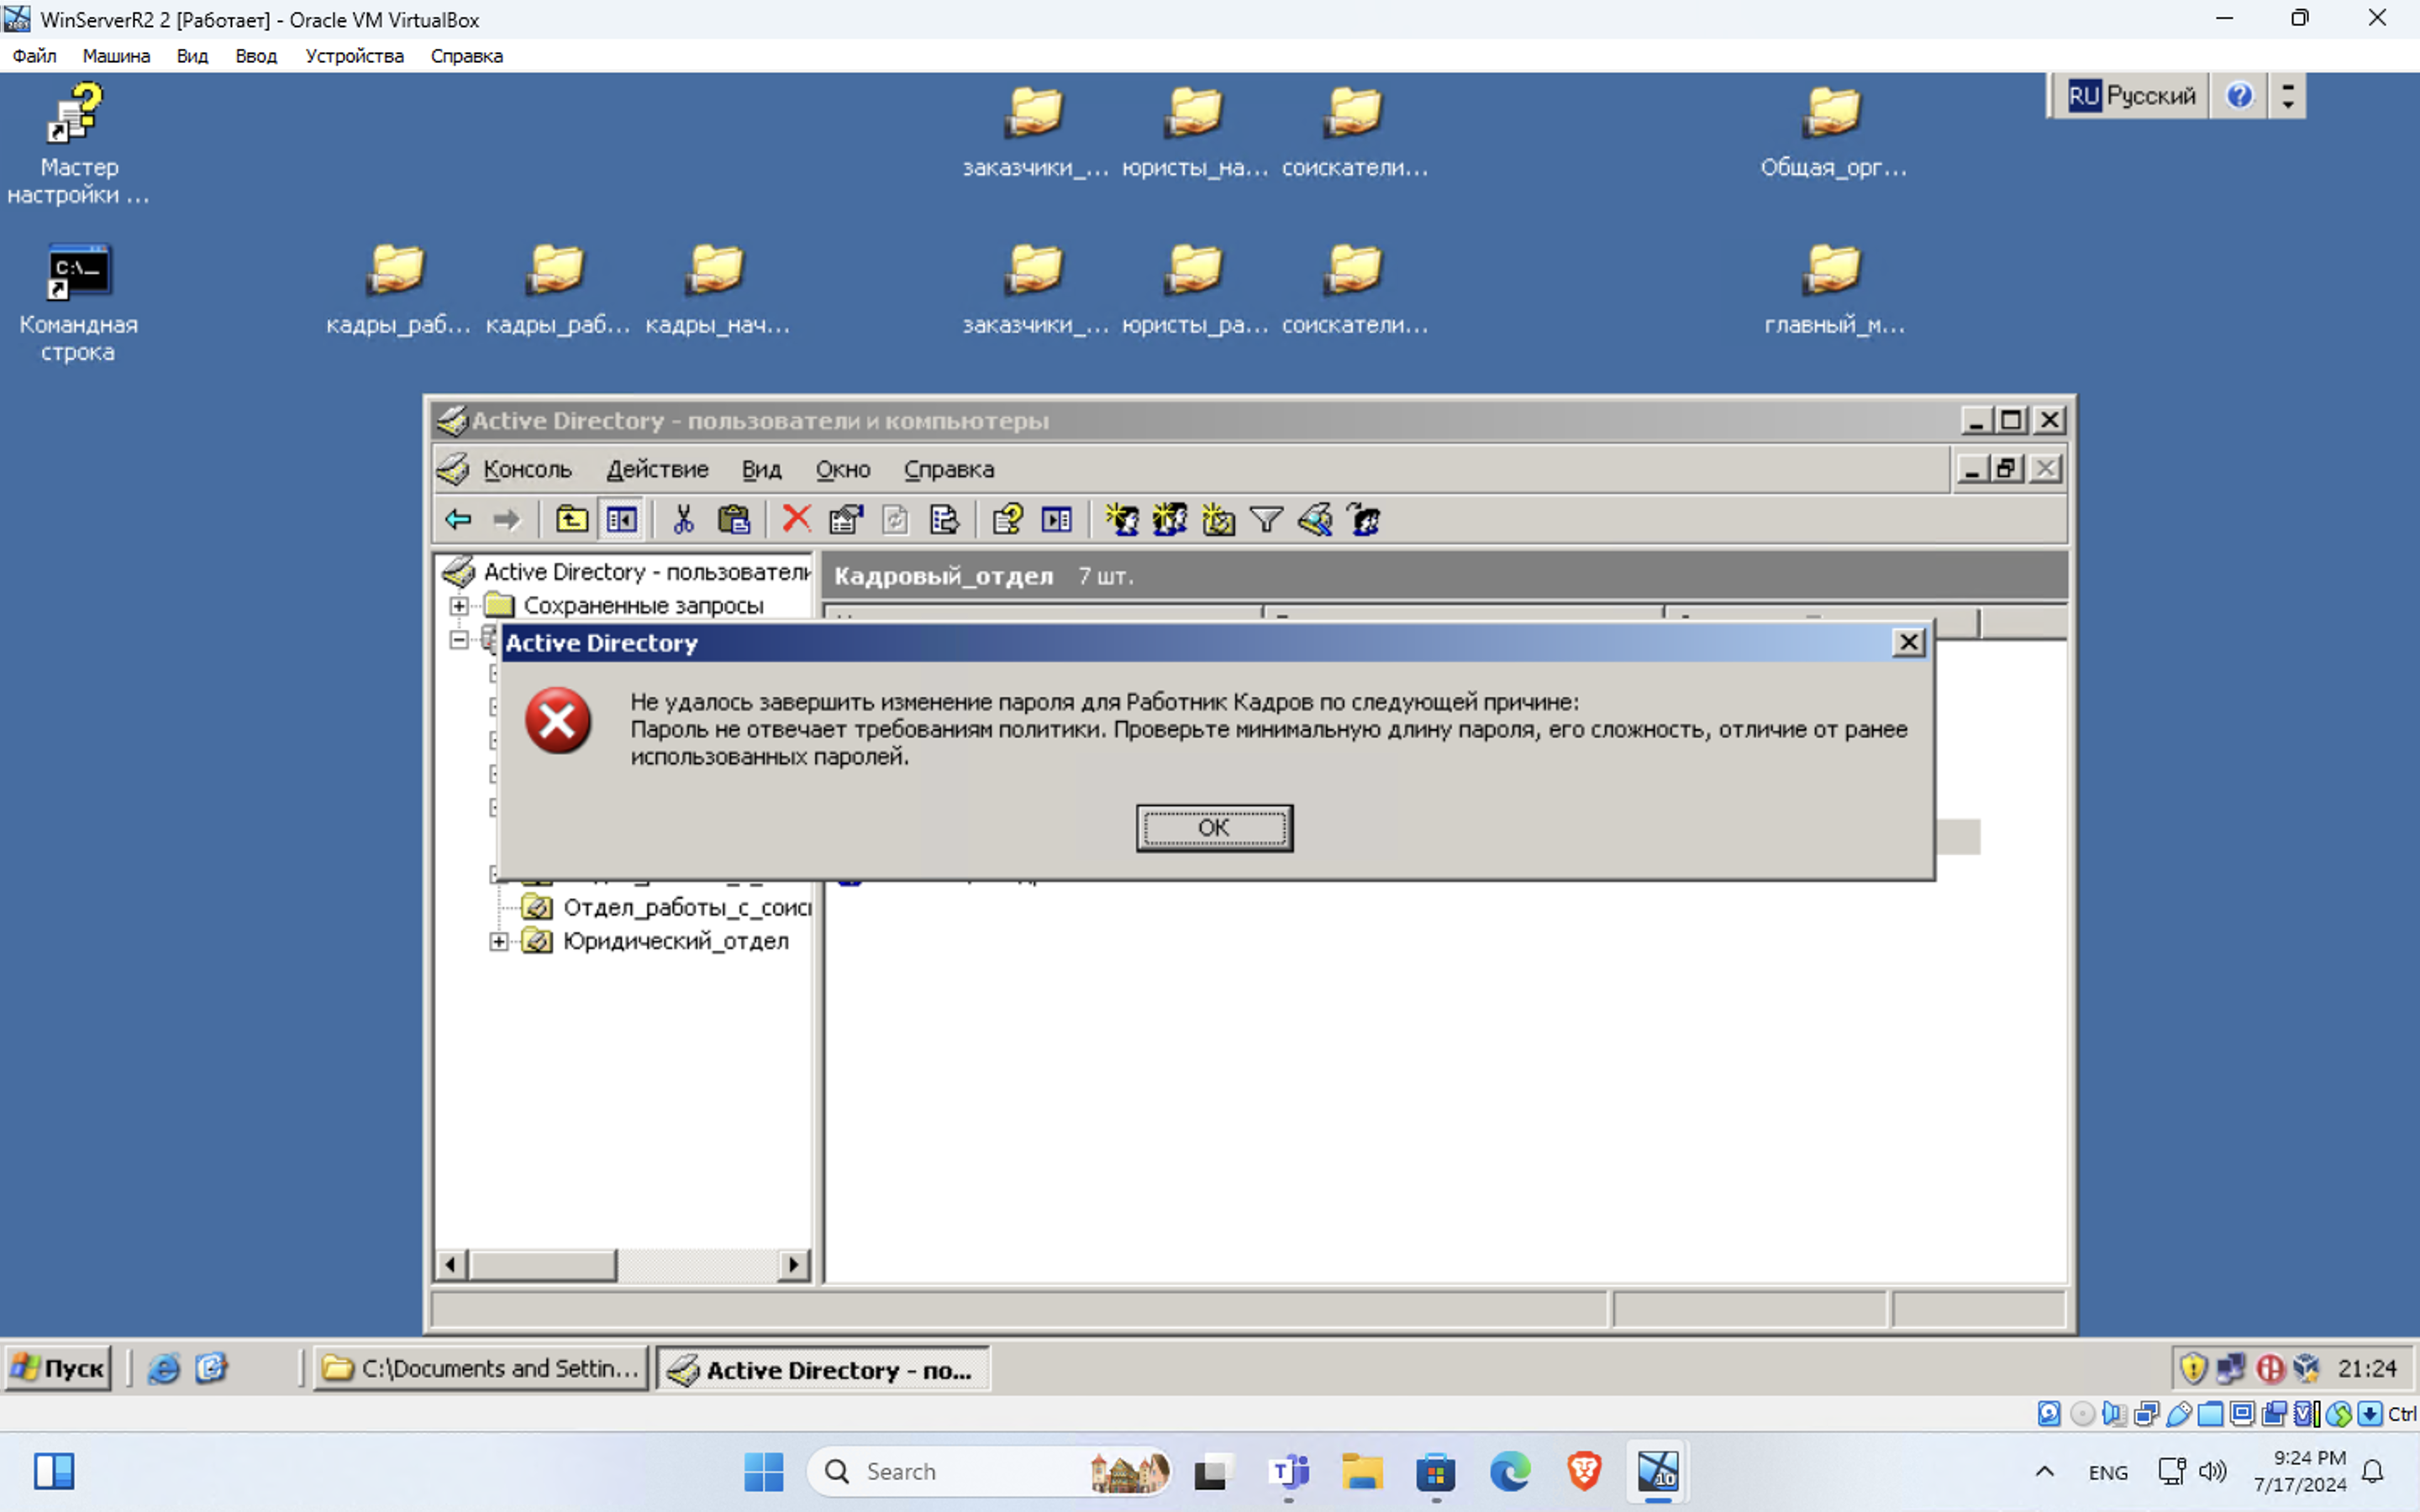
\includegraphics[width=0.9\textwidth]{pict/prac/51}
  \caption{Реакция системы на смену пароля}
  \label{fig:51}
\end{figure}

Создадим настройку ограниченного доступа к журналу, соответствующую требованию к уровню защищенности ИС.
\begin{figure}[H]
  \centering
  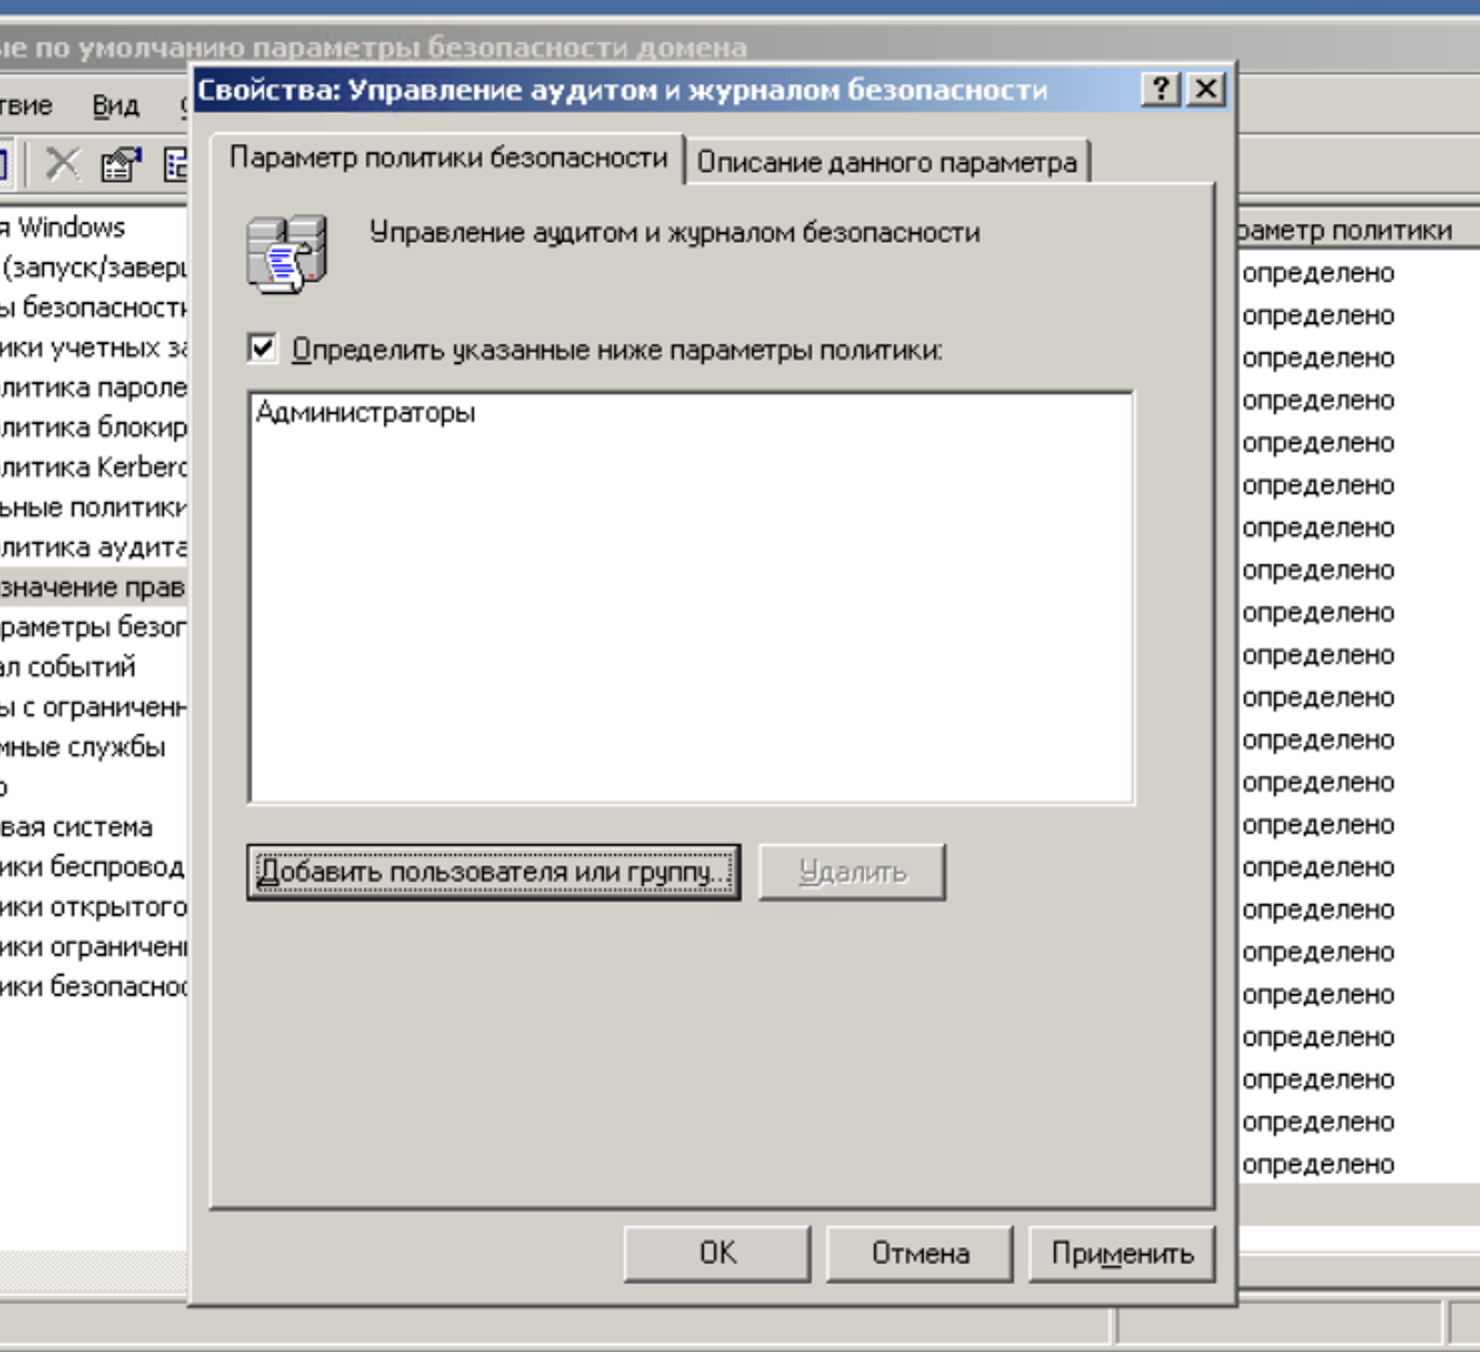
\includegraphics[width=1\textwidth]{pict/prac/59}
  \caption{Ограничение доступа к журналу}
\end{figure}

Зайдем в аккаунт одного оз пользователей и попробуем посмотреть журнал безопасность.
\begin{figure}[H]
  \centering
  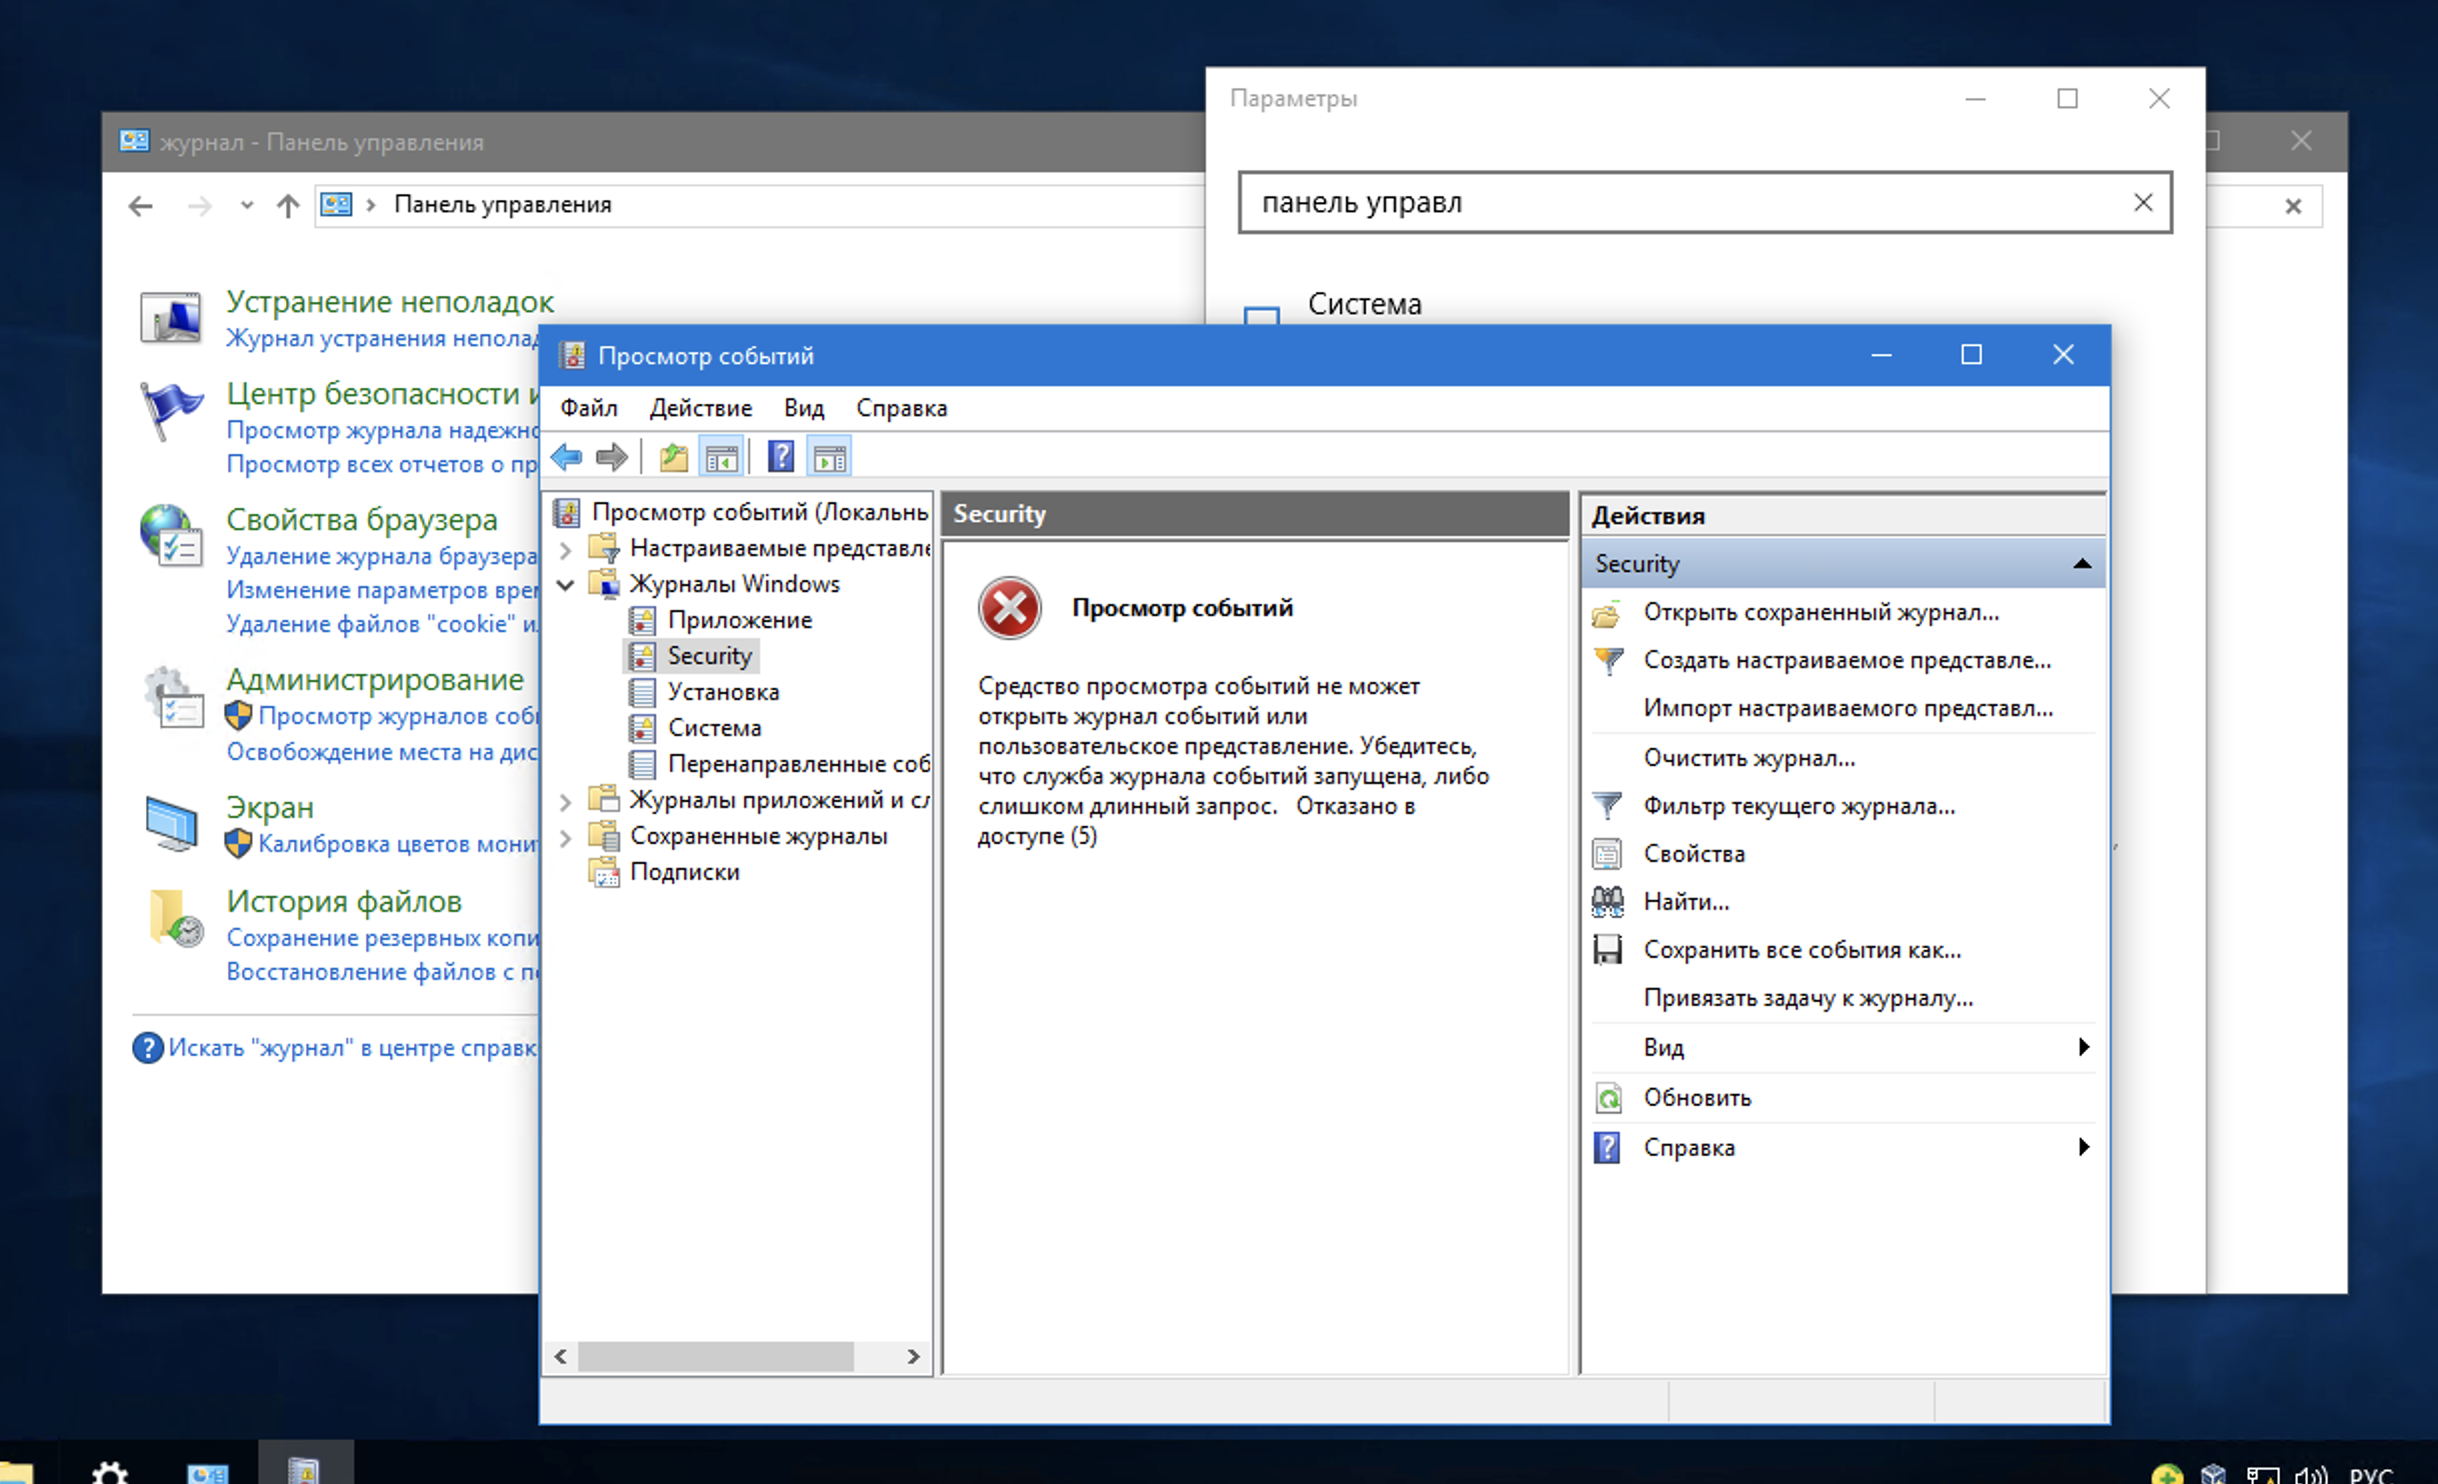
\includegraphics[width=1\textwidth]{pict/prac/80}
  \caption{Реакция на доступ к журналу}
\end{figure}

Также чтобы в систему имели доступ только аутентифицированные пользователи, отключим учетную запись гостя.

\begin{figure}[H]
  \centering
  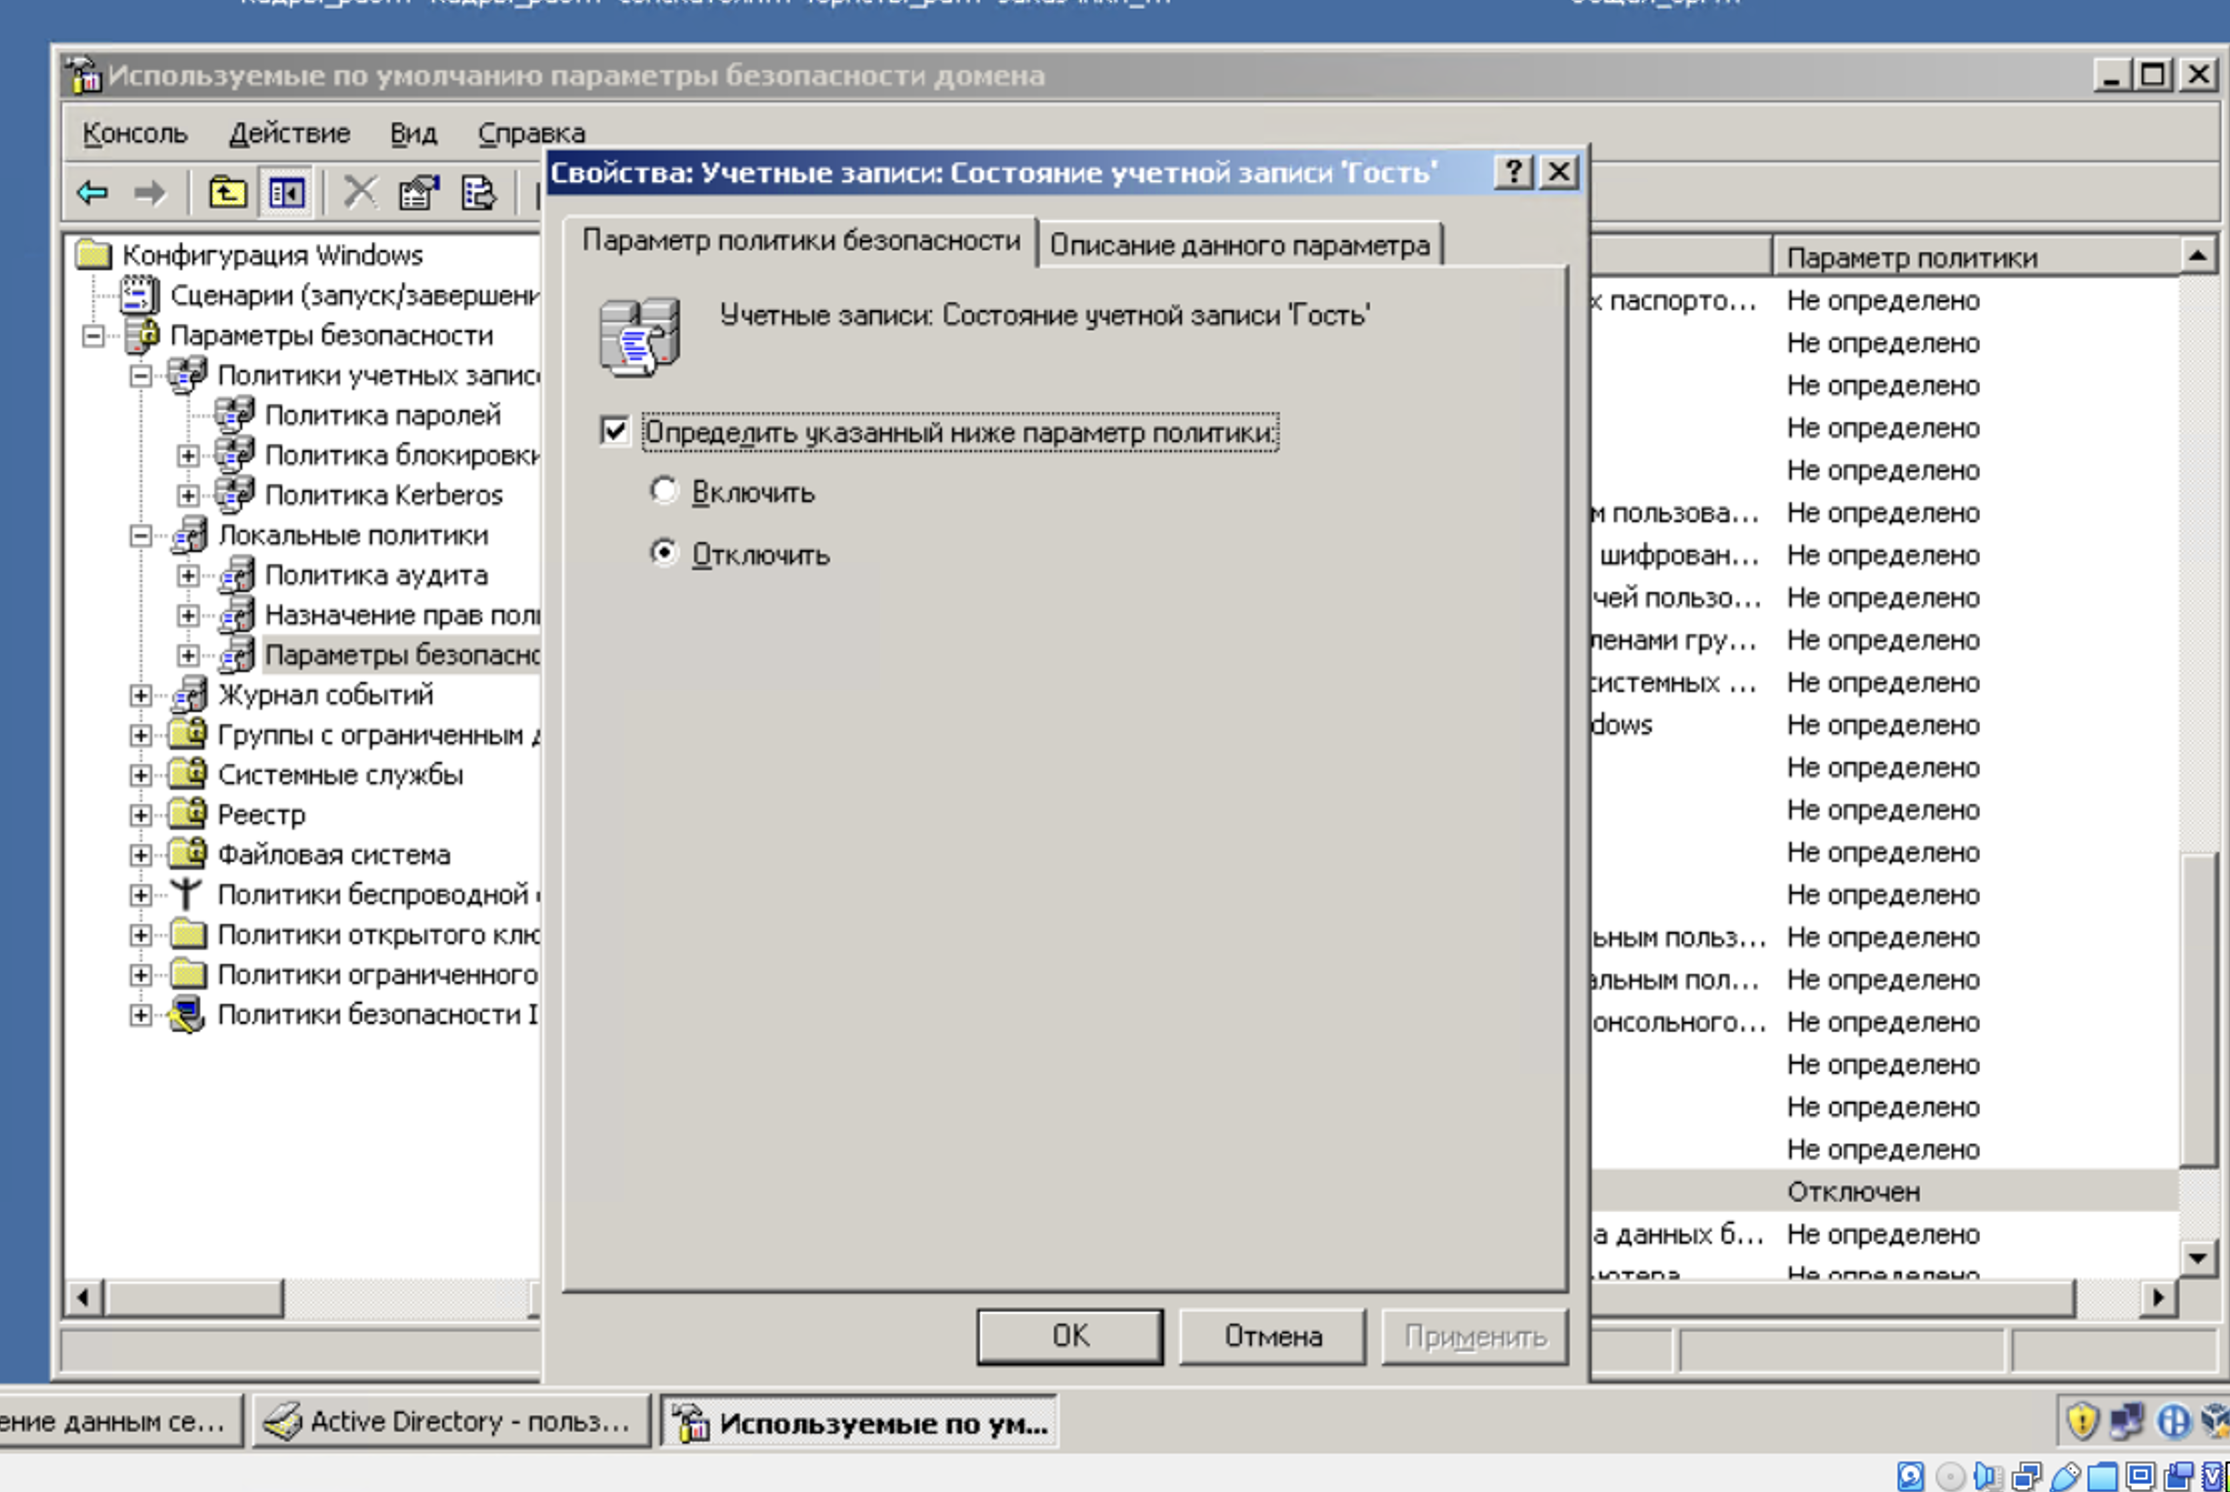
\includegraphics[width=1\textwidth]{pict/prac/60}
  \caption{Запрет гостевой учетной записи}
\end{figure}

Проверим работ предыдущей политики.
\begin{figure}[H]
  \centering
  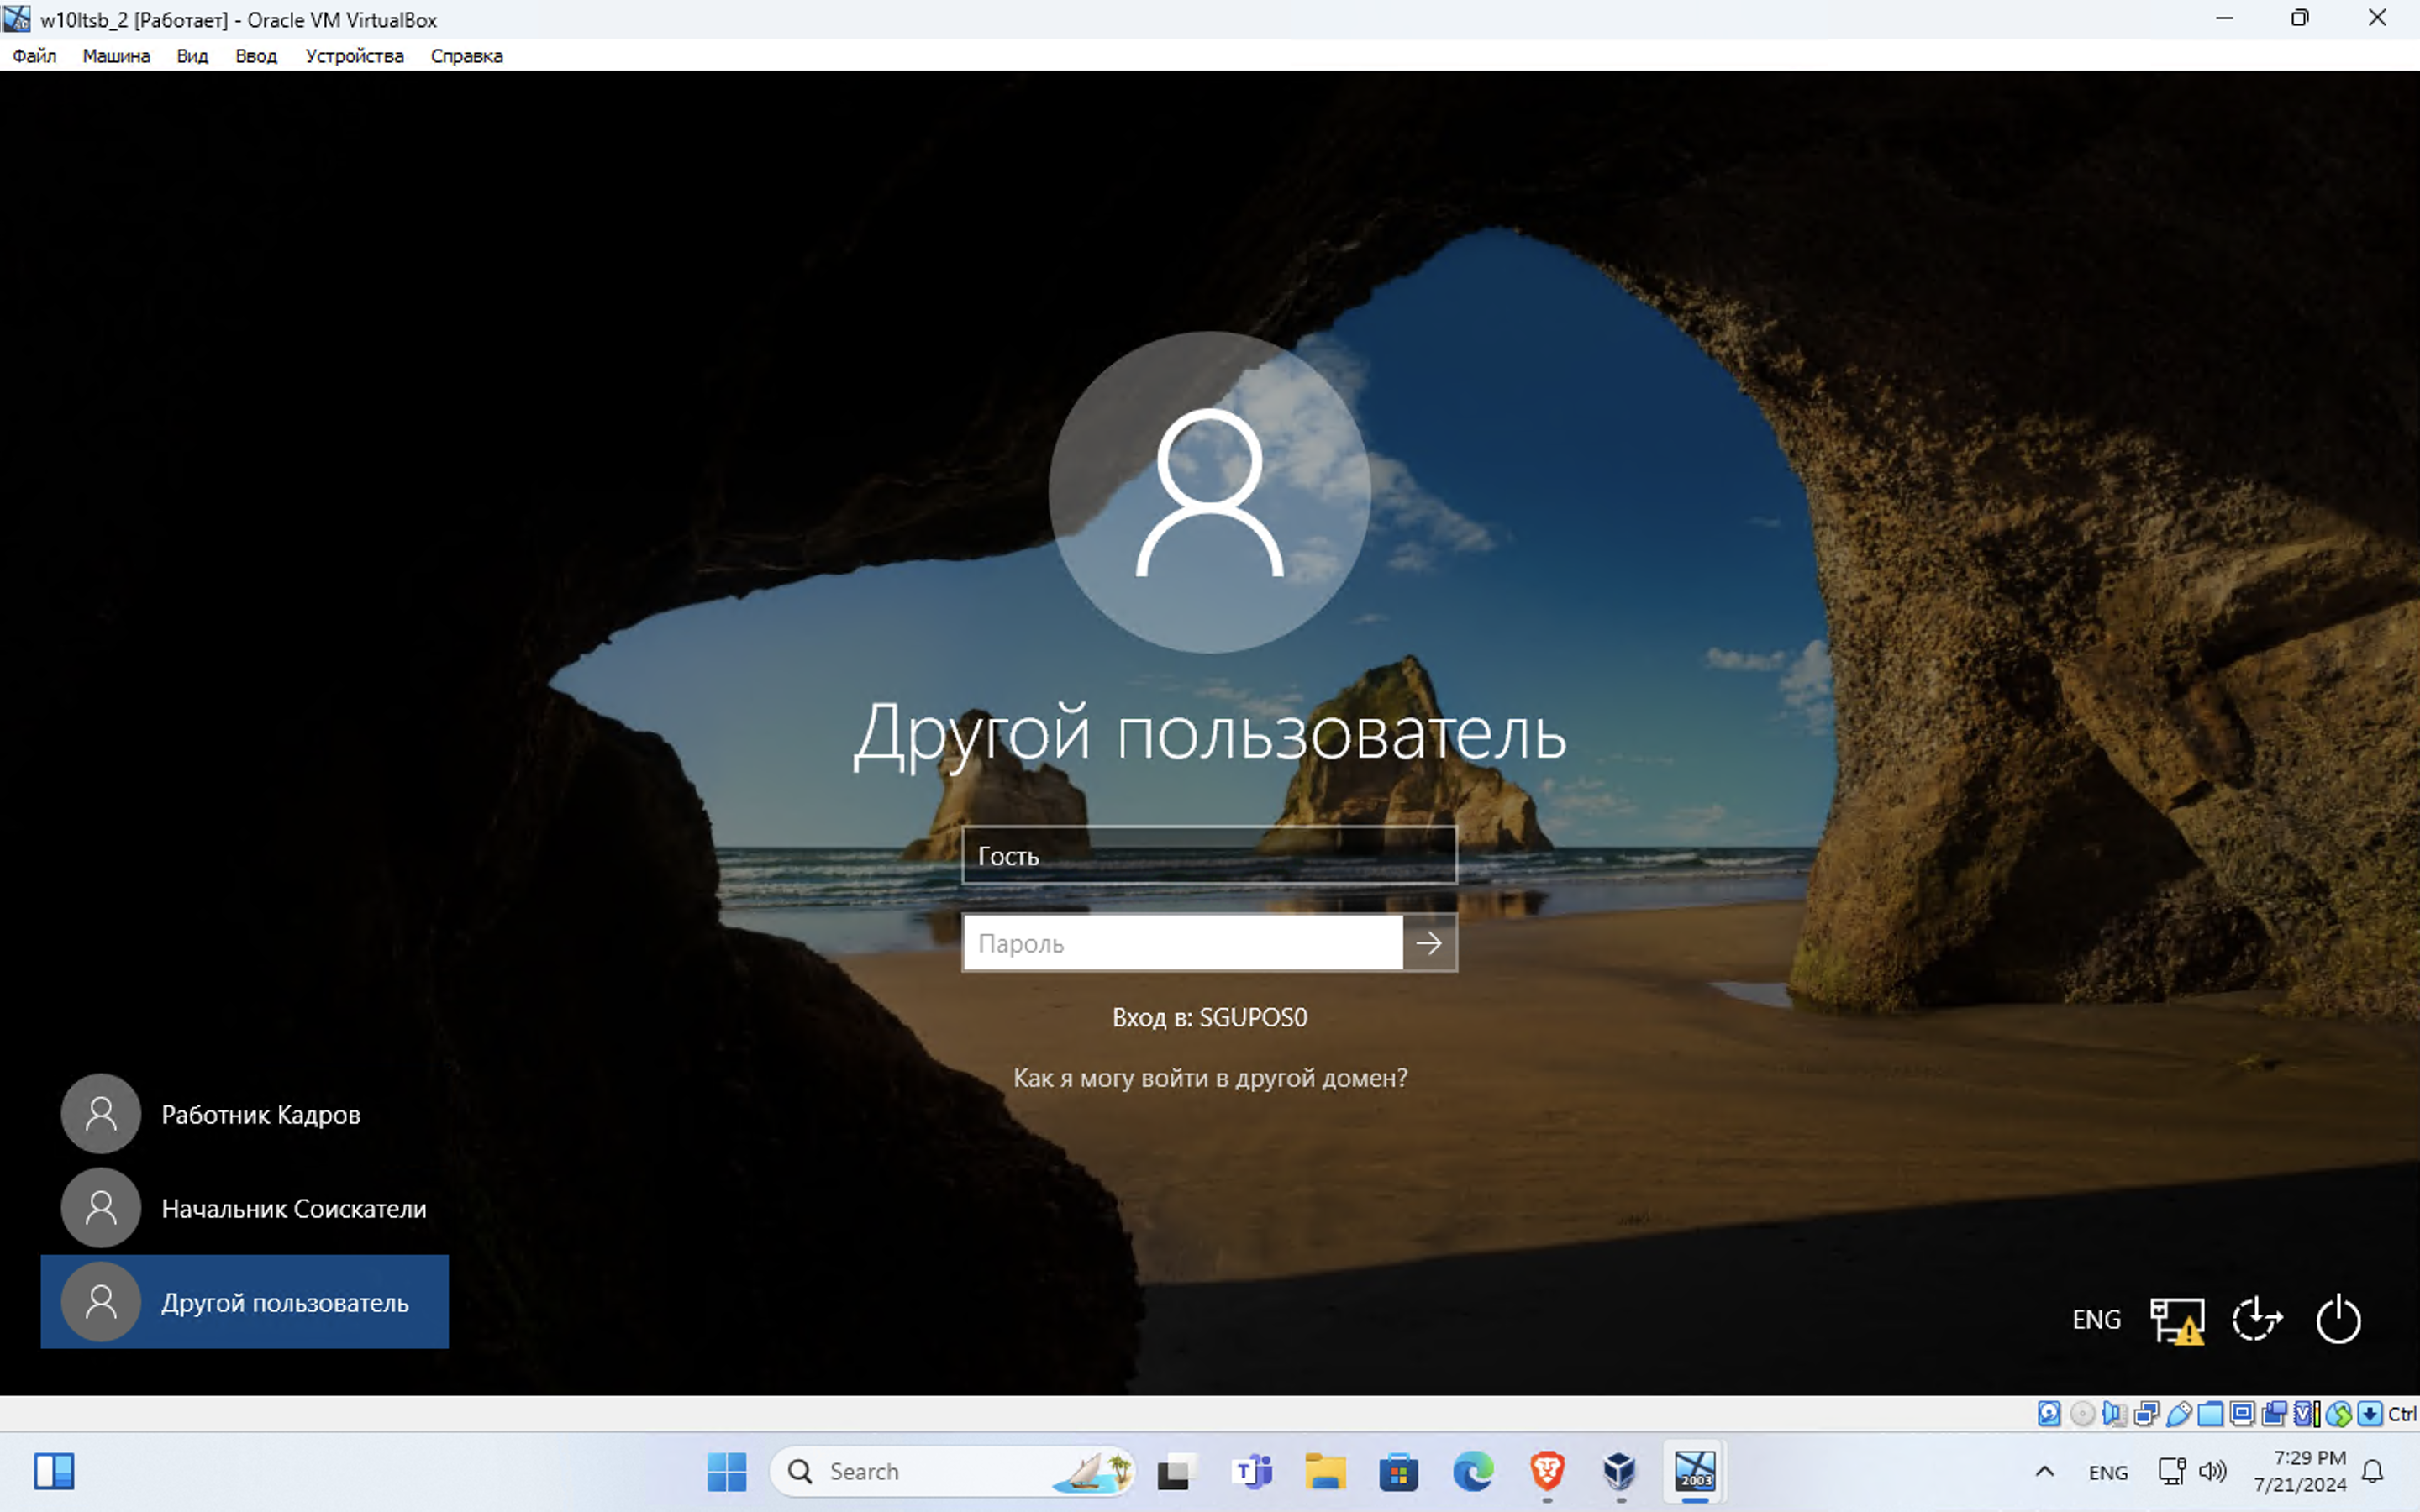
\includegraphics[width=1\textwidth]{pict/prac/65}
  \caption{Реакция системы на вход гостя}
\end{figure}

\begin{figure}[H]
  \centering
  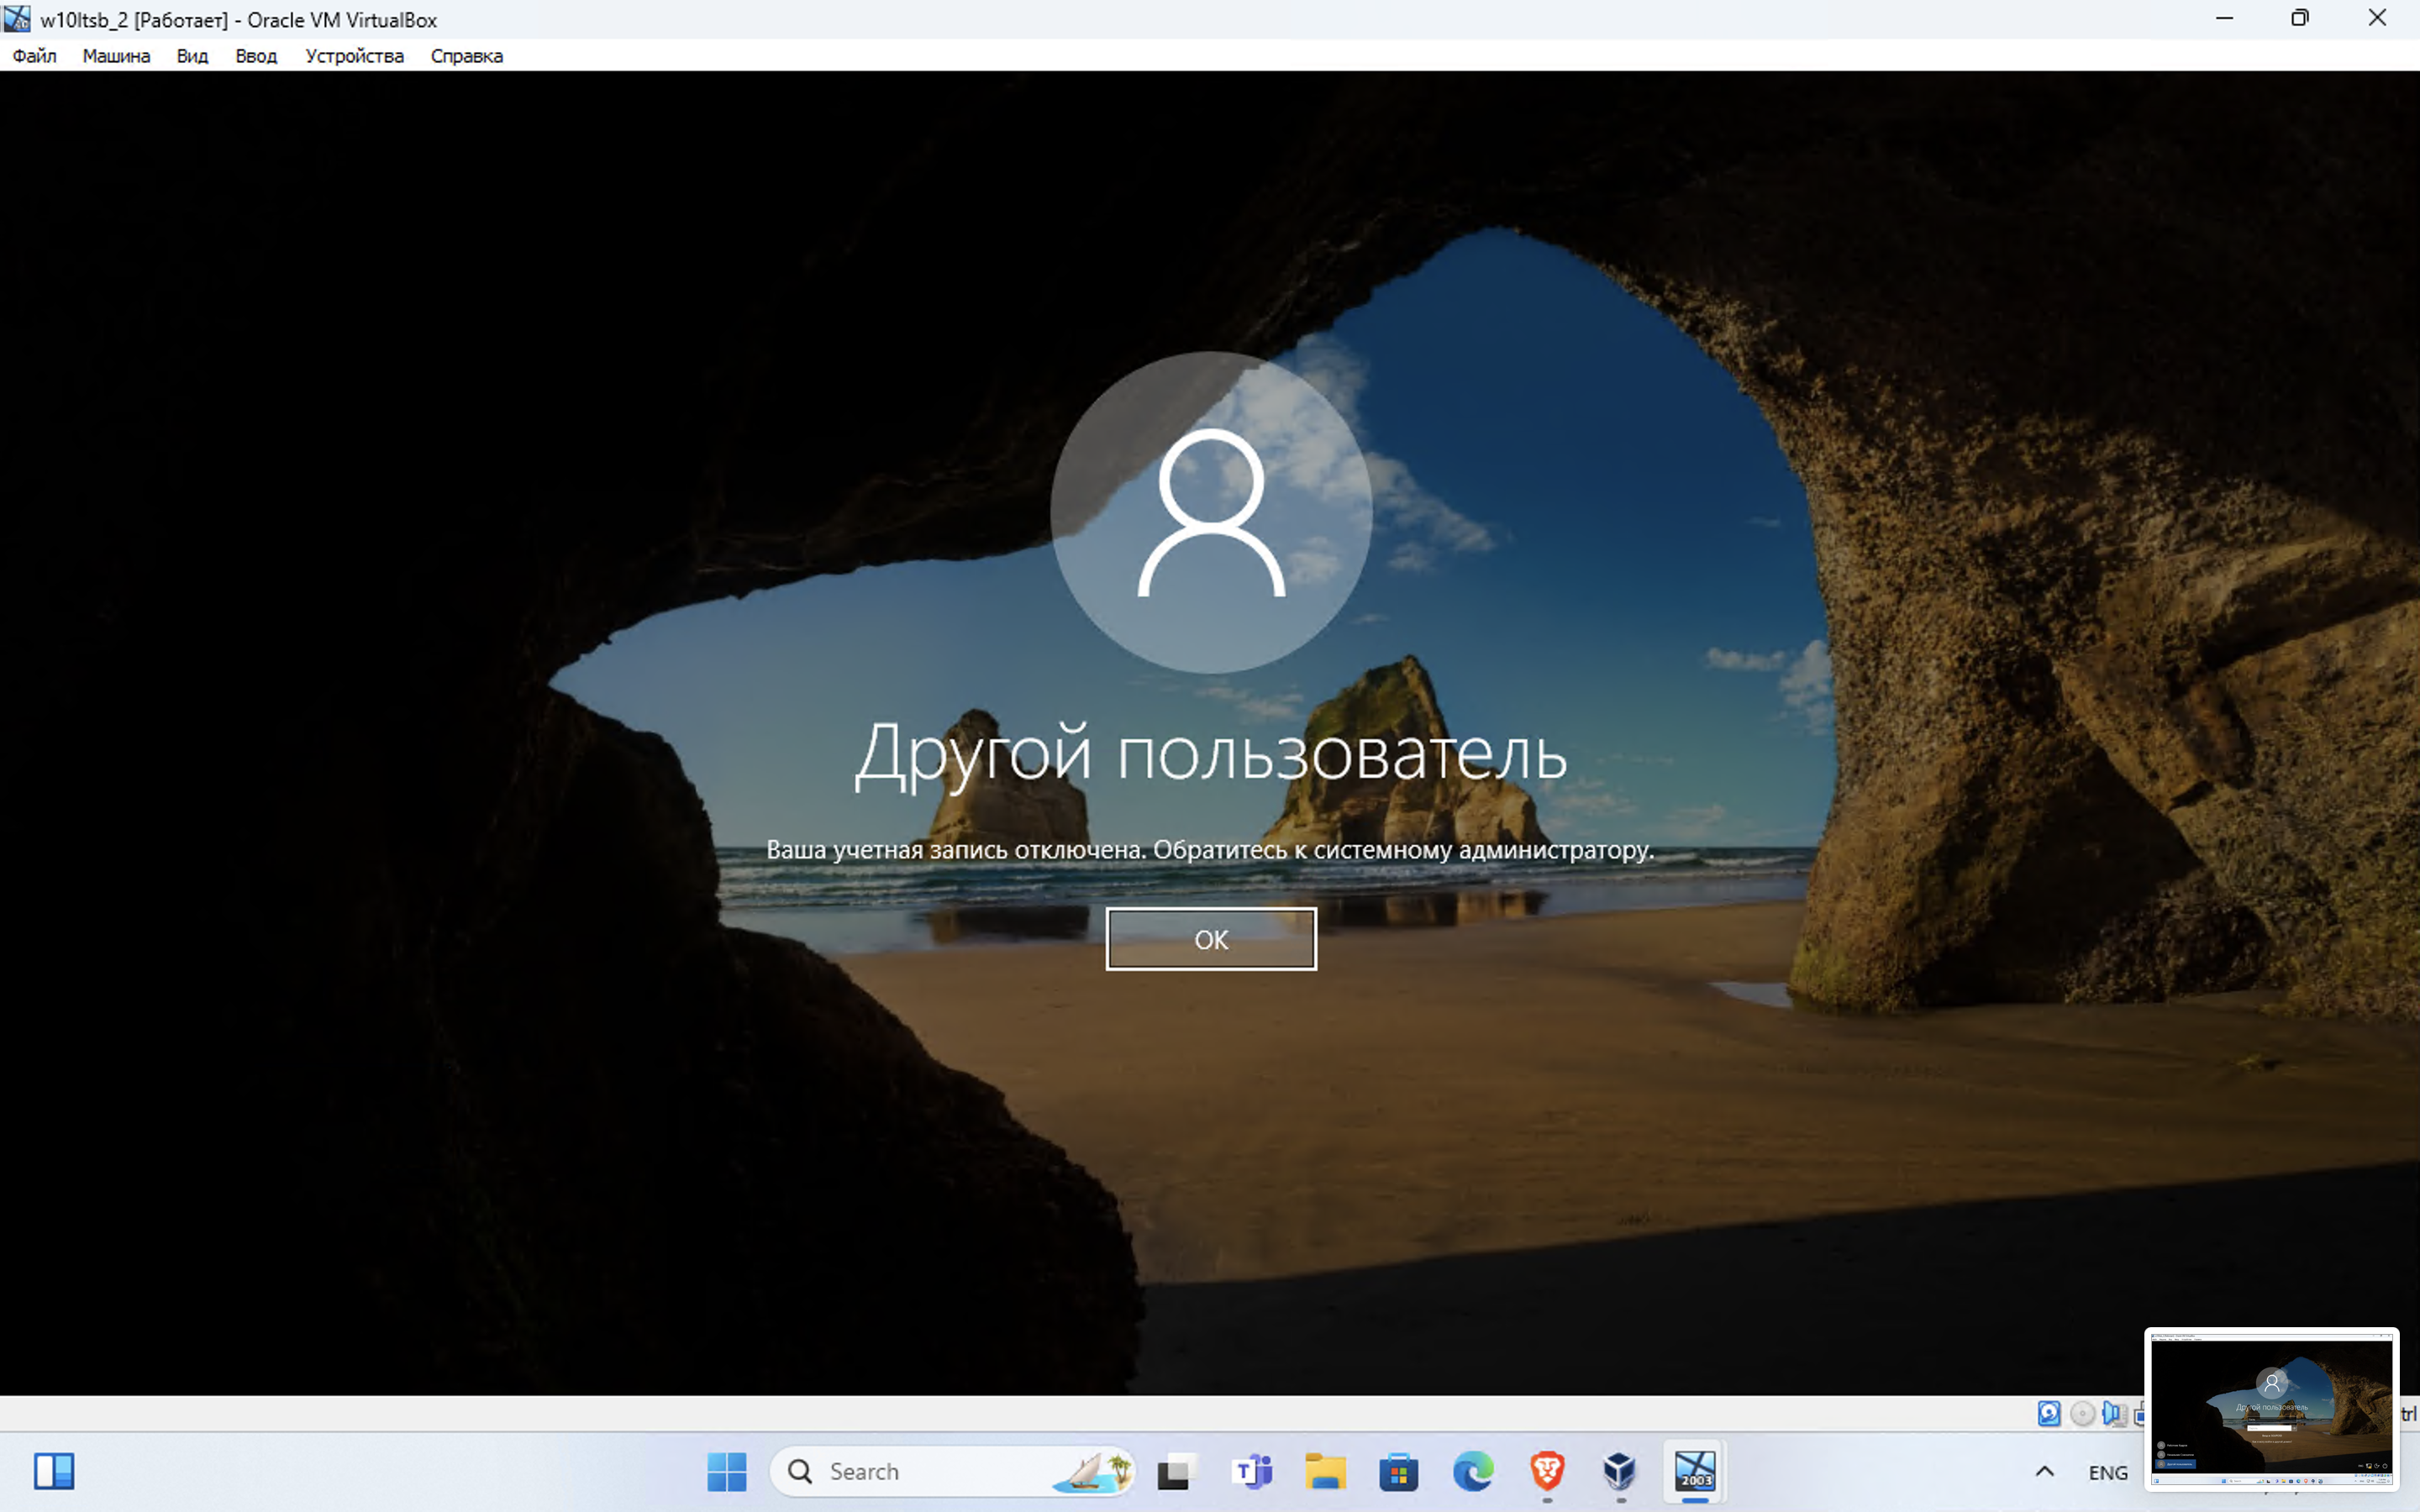
\includegraphics[width=1\textwidth]{pict/prac/66}
  \caption{Реакция системы на вход гостя}
\end{figure}

Аналогично создадим всех остальных пользователей для каждого подразделения.

\begin{figure}[H]
  \centering
  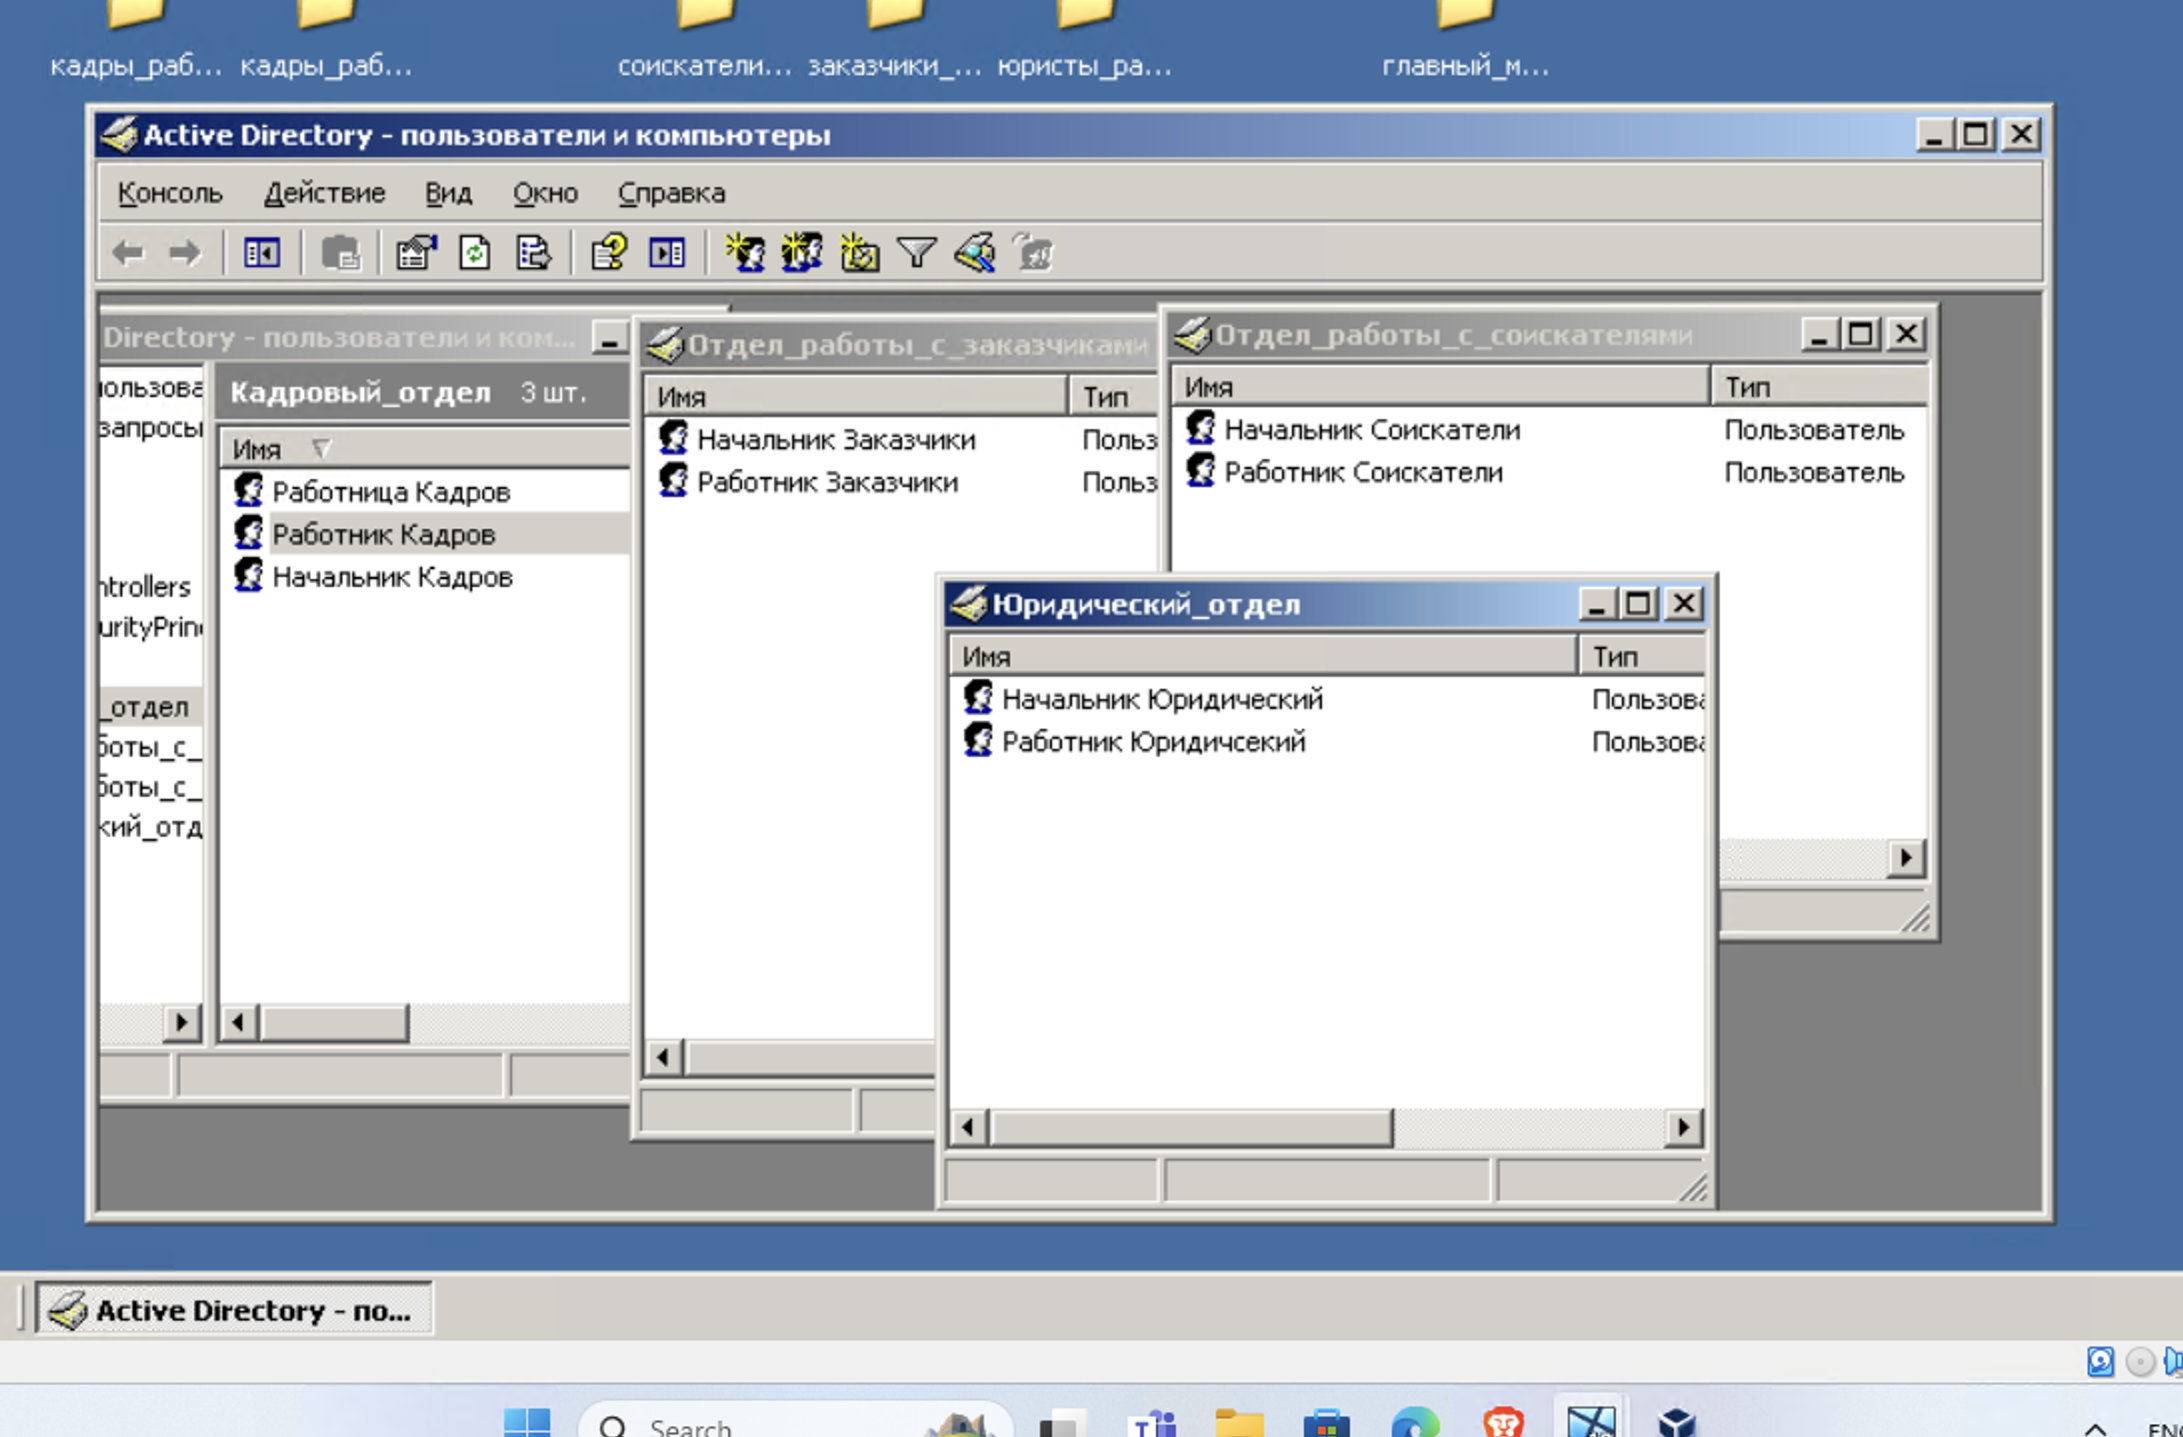
\includegraphics[width=0.9\textwidth]{pict/prac/4}
  \caption{Аккаунты работников}
  \label{fig:15}
\end{figure}

Создадим сетевой ресурс для общей папки во всех отделах, так как папка нужна для обмена данными, то 
все имеют право туда писать, читать, но изменять содержимое чужих файлов нет.

\begin{figure}[H]
  \centering
  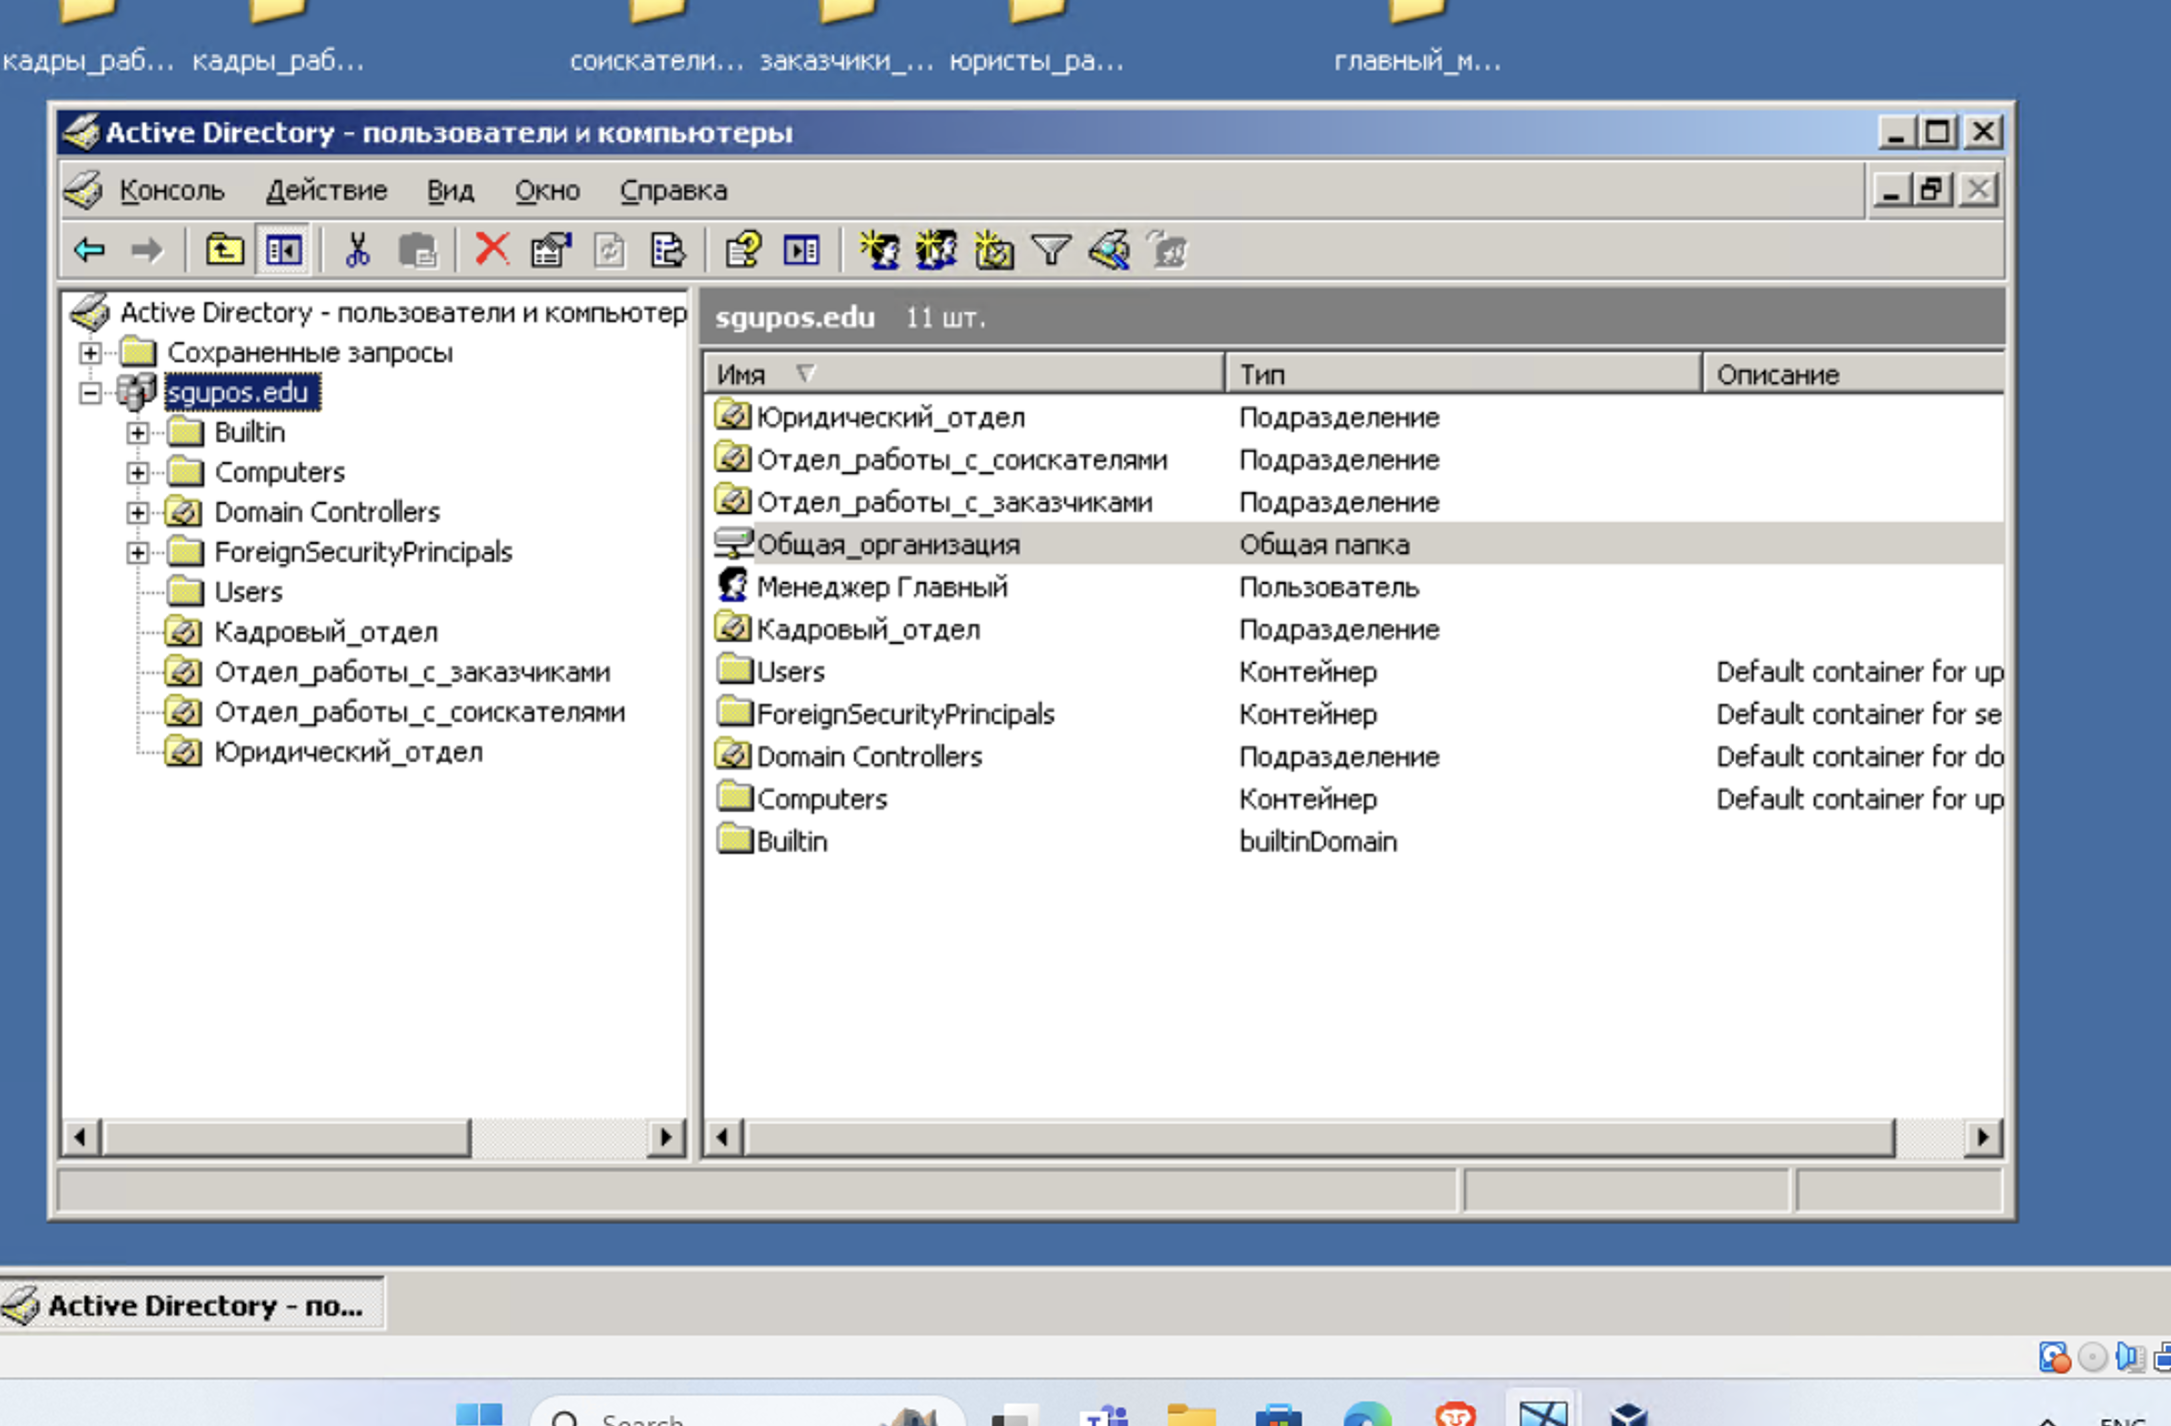
\includegraphics[width=0.9\textwidth]{pict/prac/5}
  \caption{Общая папка}
  \label{fig:16}
\end{figure}

\begin{figure}[H]
  \centering
  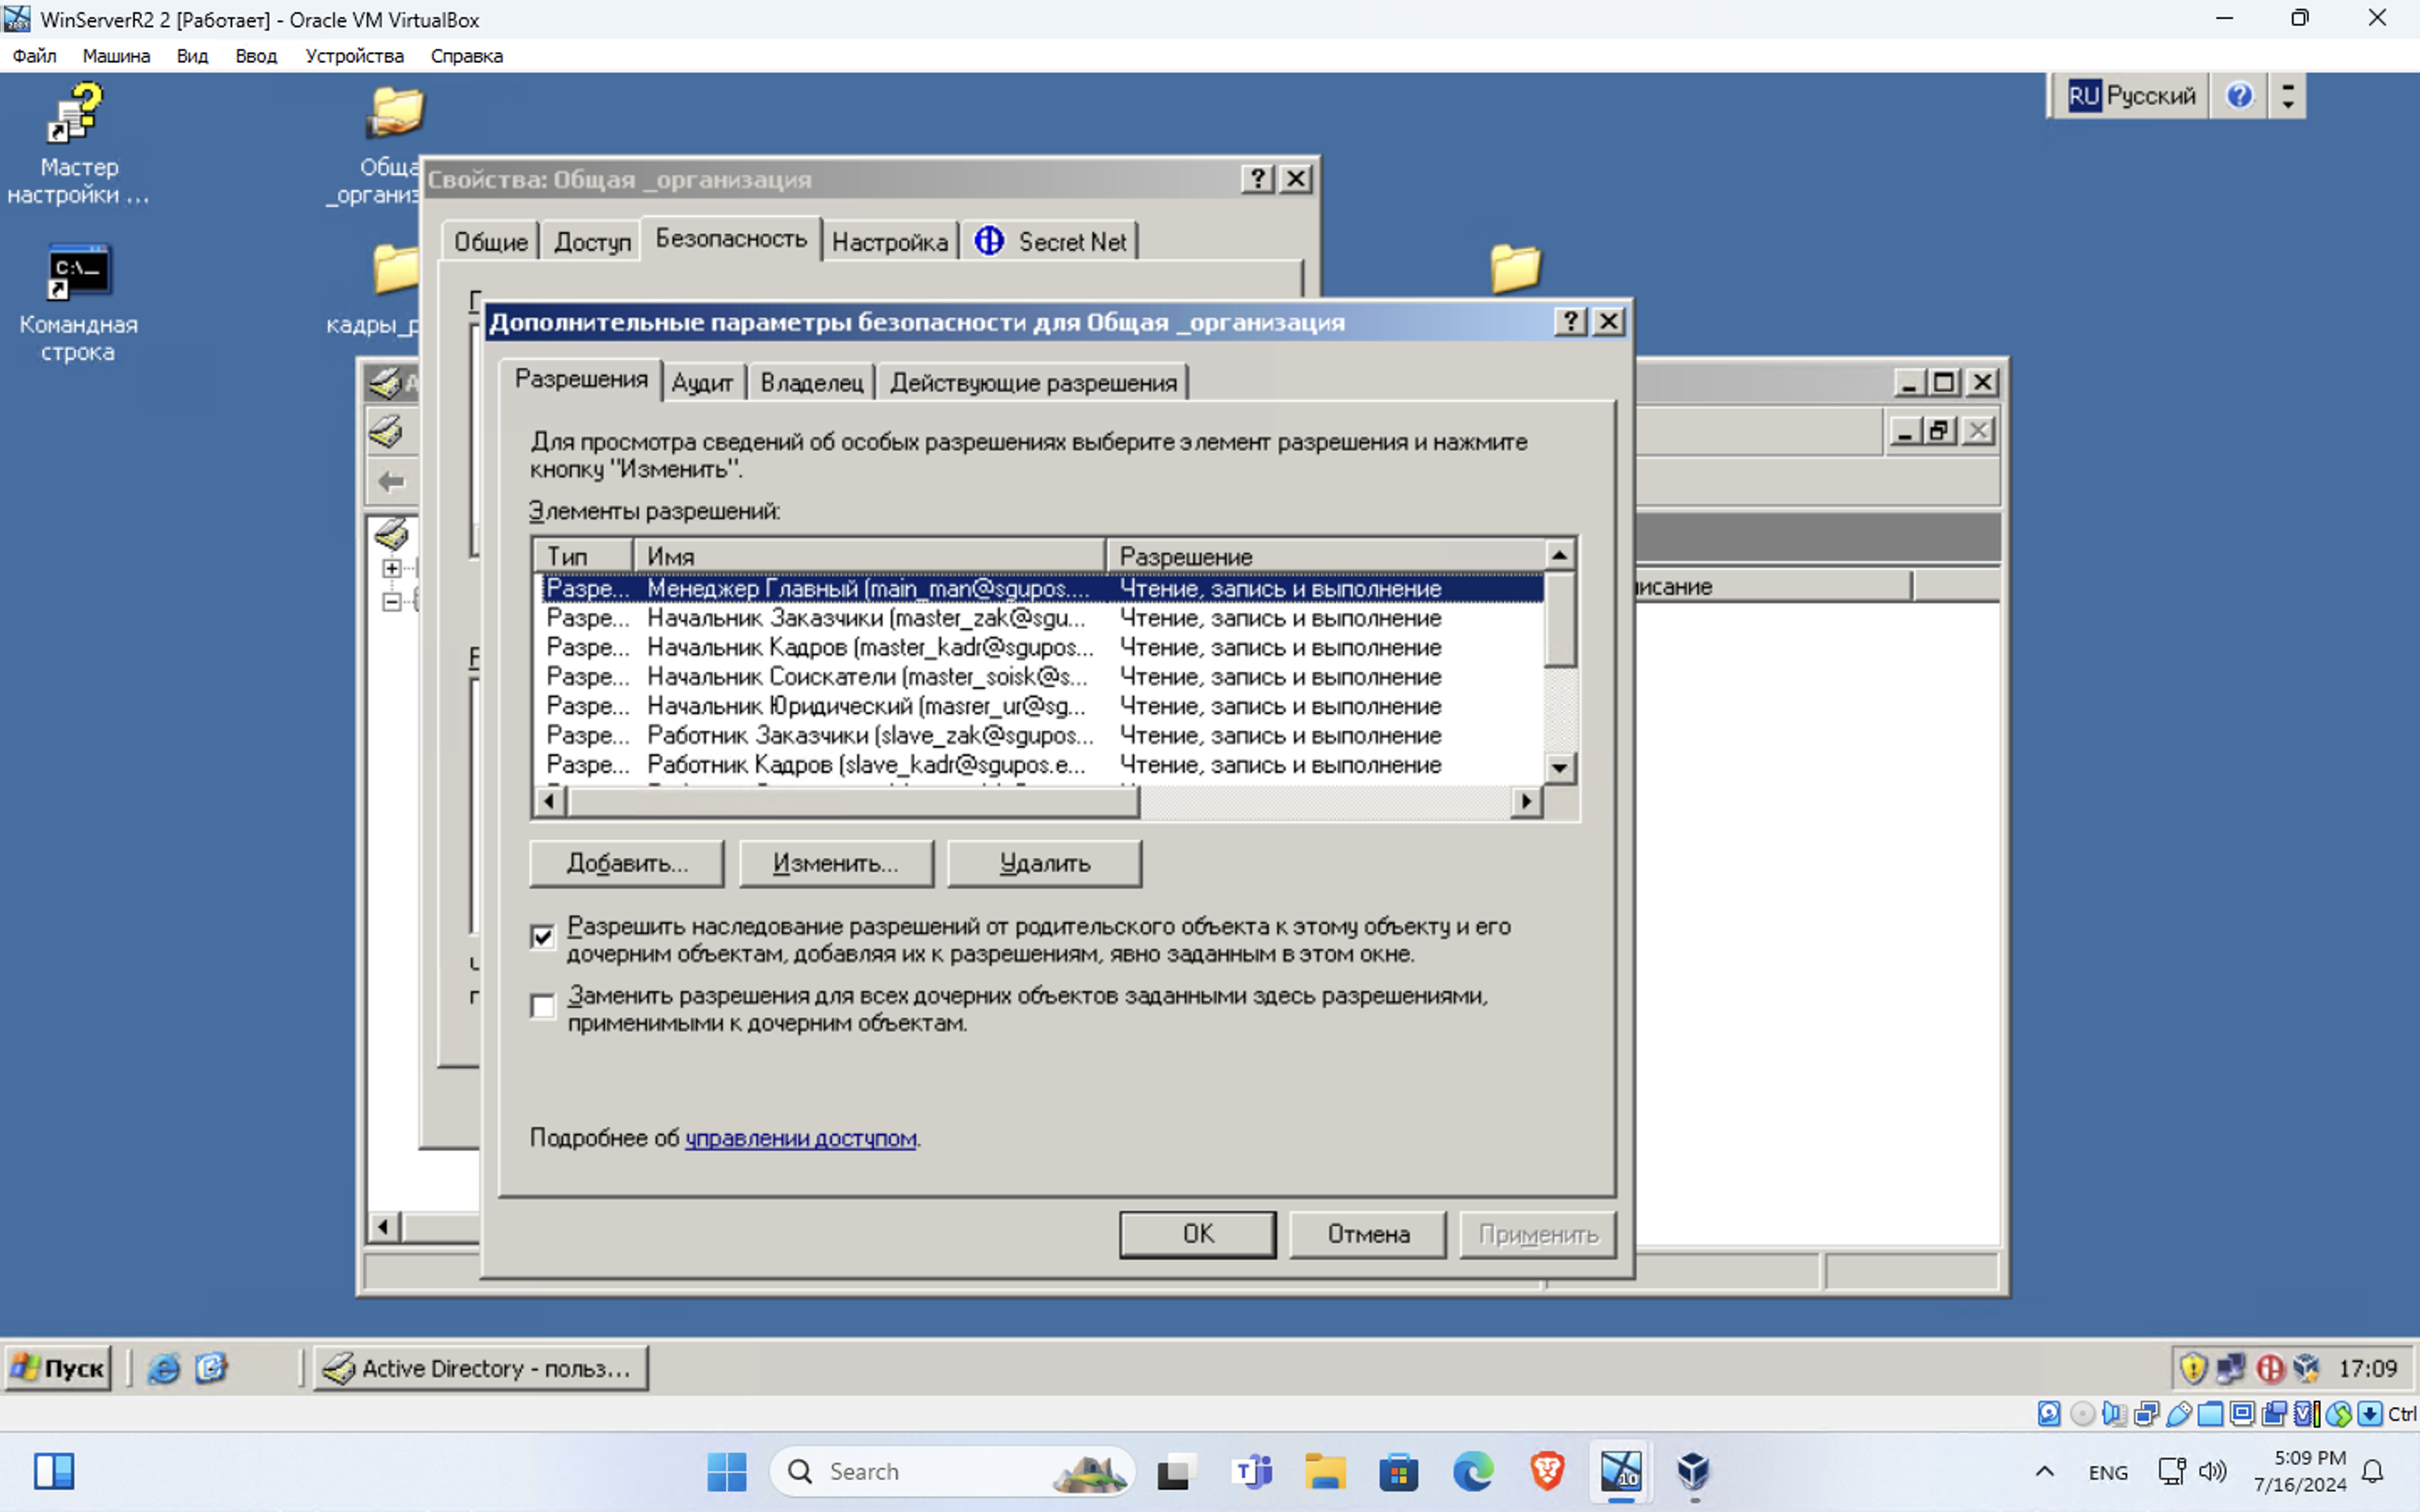
\includegraphics[width=0.9\textwidth]{pict/prac/6}
  \caption{Права на общую папку}
  \label{fig:17}
\end{figure}


Также создадим в каждом подразделении будет сетевой ресурс, указывающий на общую папку.
\begin{figure}[H]
  \centering
  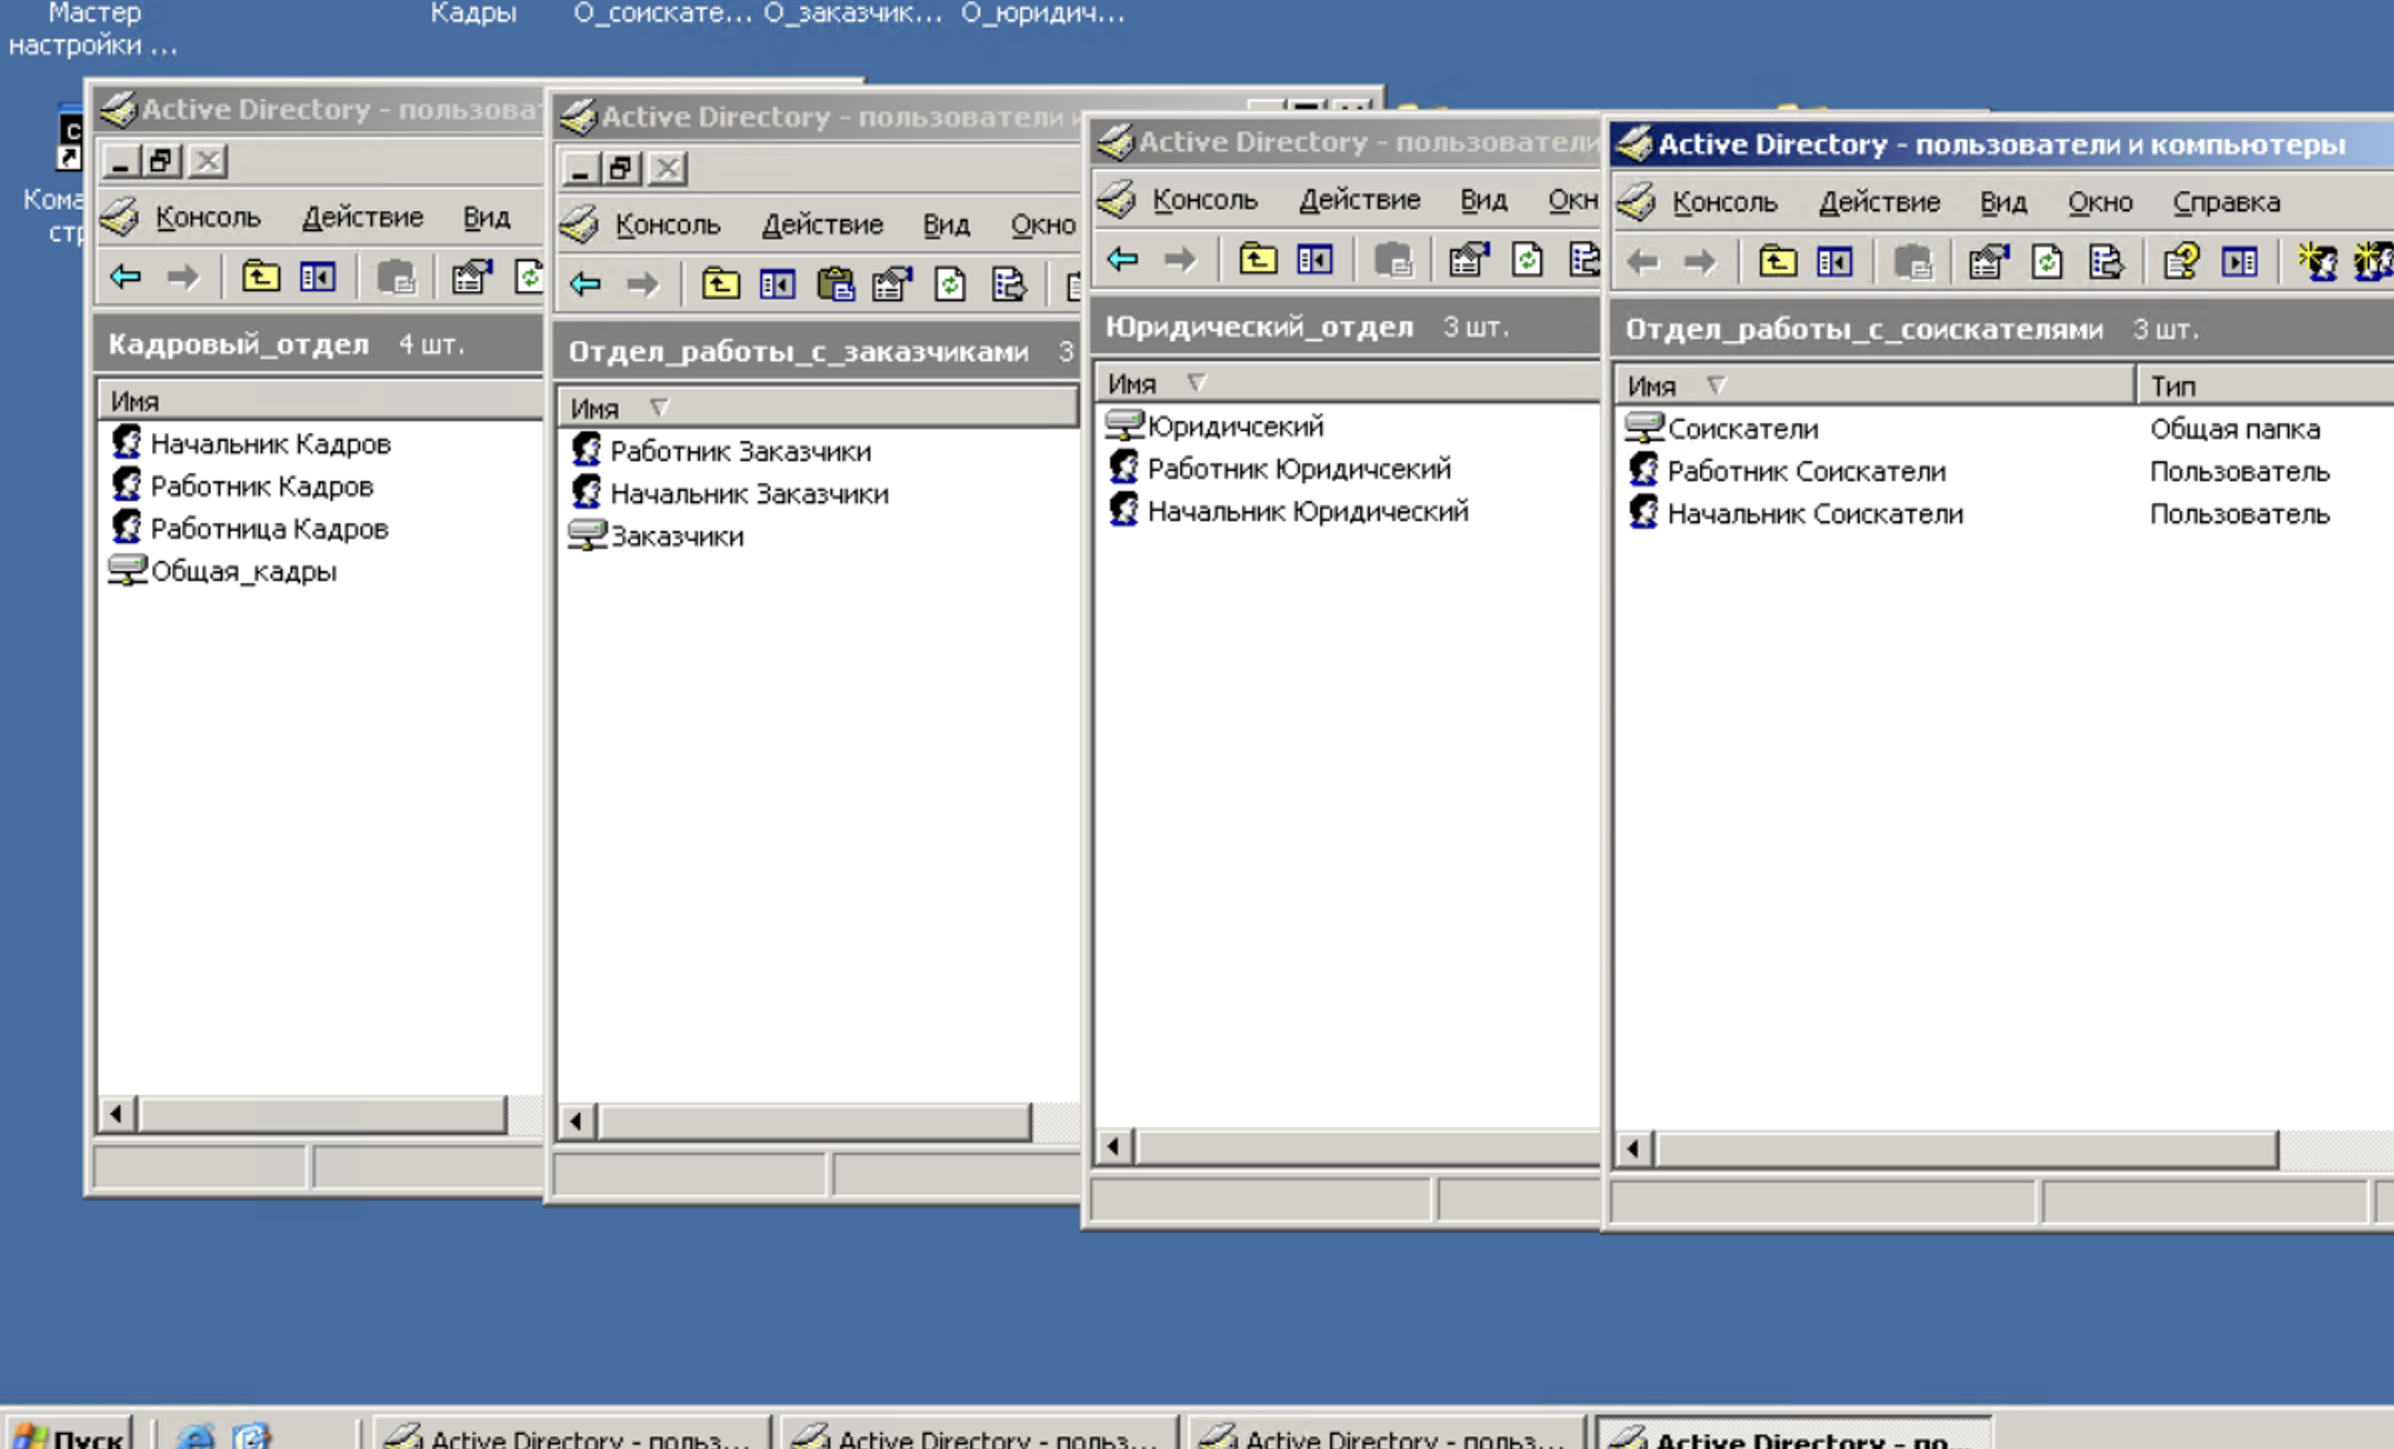
\includegraphics[width=0.9\textwidth]{pict/prac/7}
  \caption{Общие папки}
  \label{fig:18}
\end{figure}

Для своей папки, сотрудник имеет следующие права:
\begin{figure}[H]
  \centering
  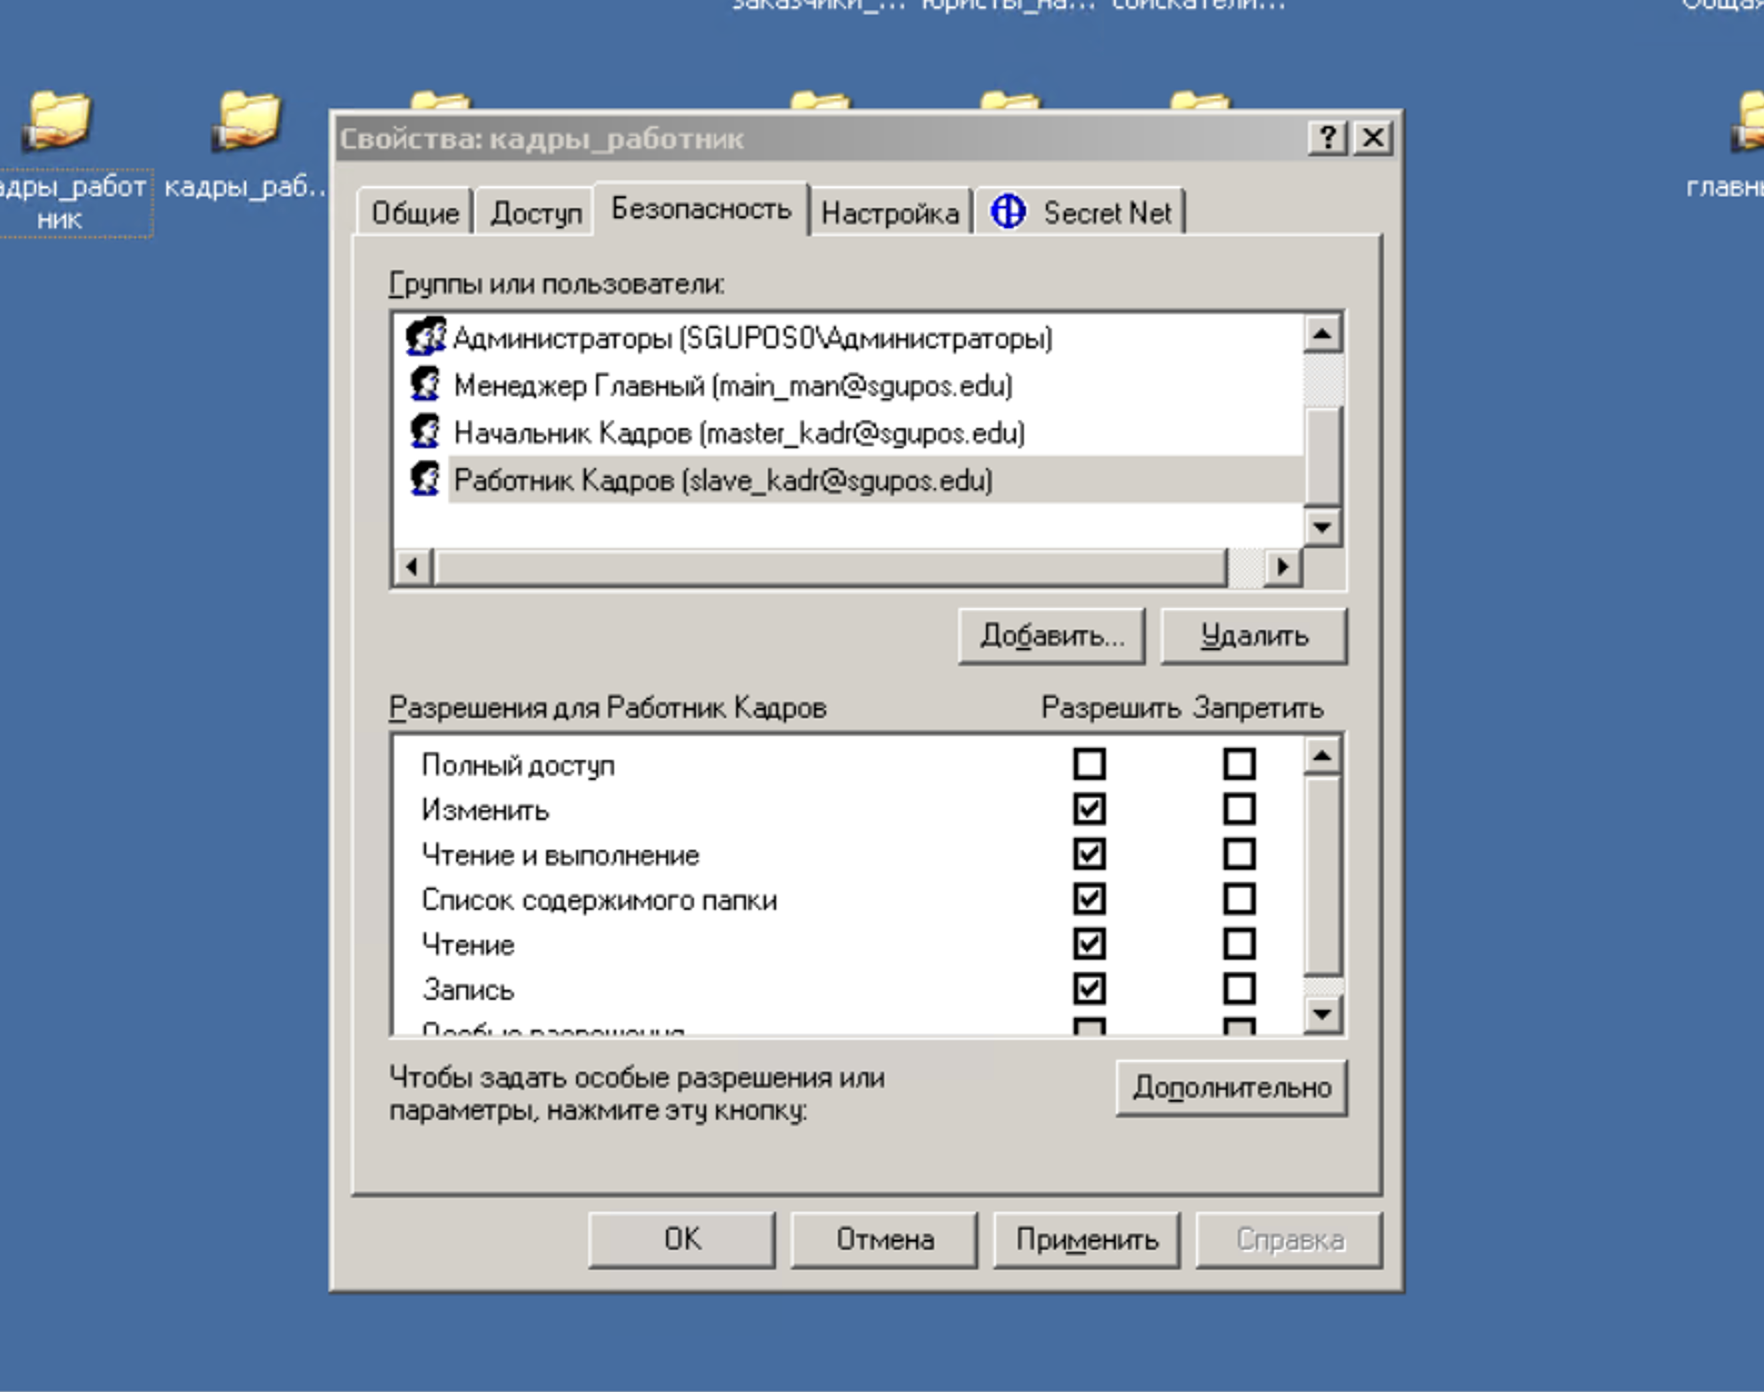
\includegraphics[width=0.9\textwidth]{pict/prac/8}
  \caption{Разрешено}
  \label{fig:20}
\end{figure}


\begin{figure}[H]
  \centering
  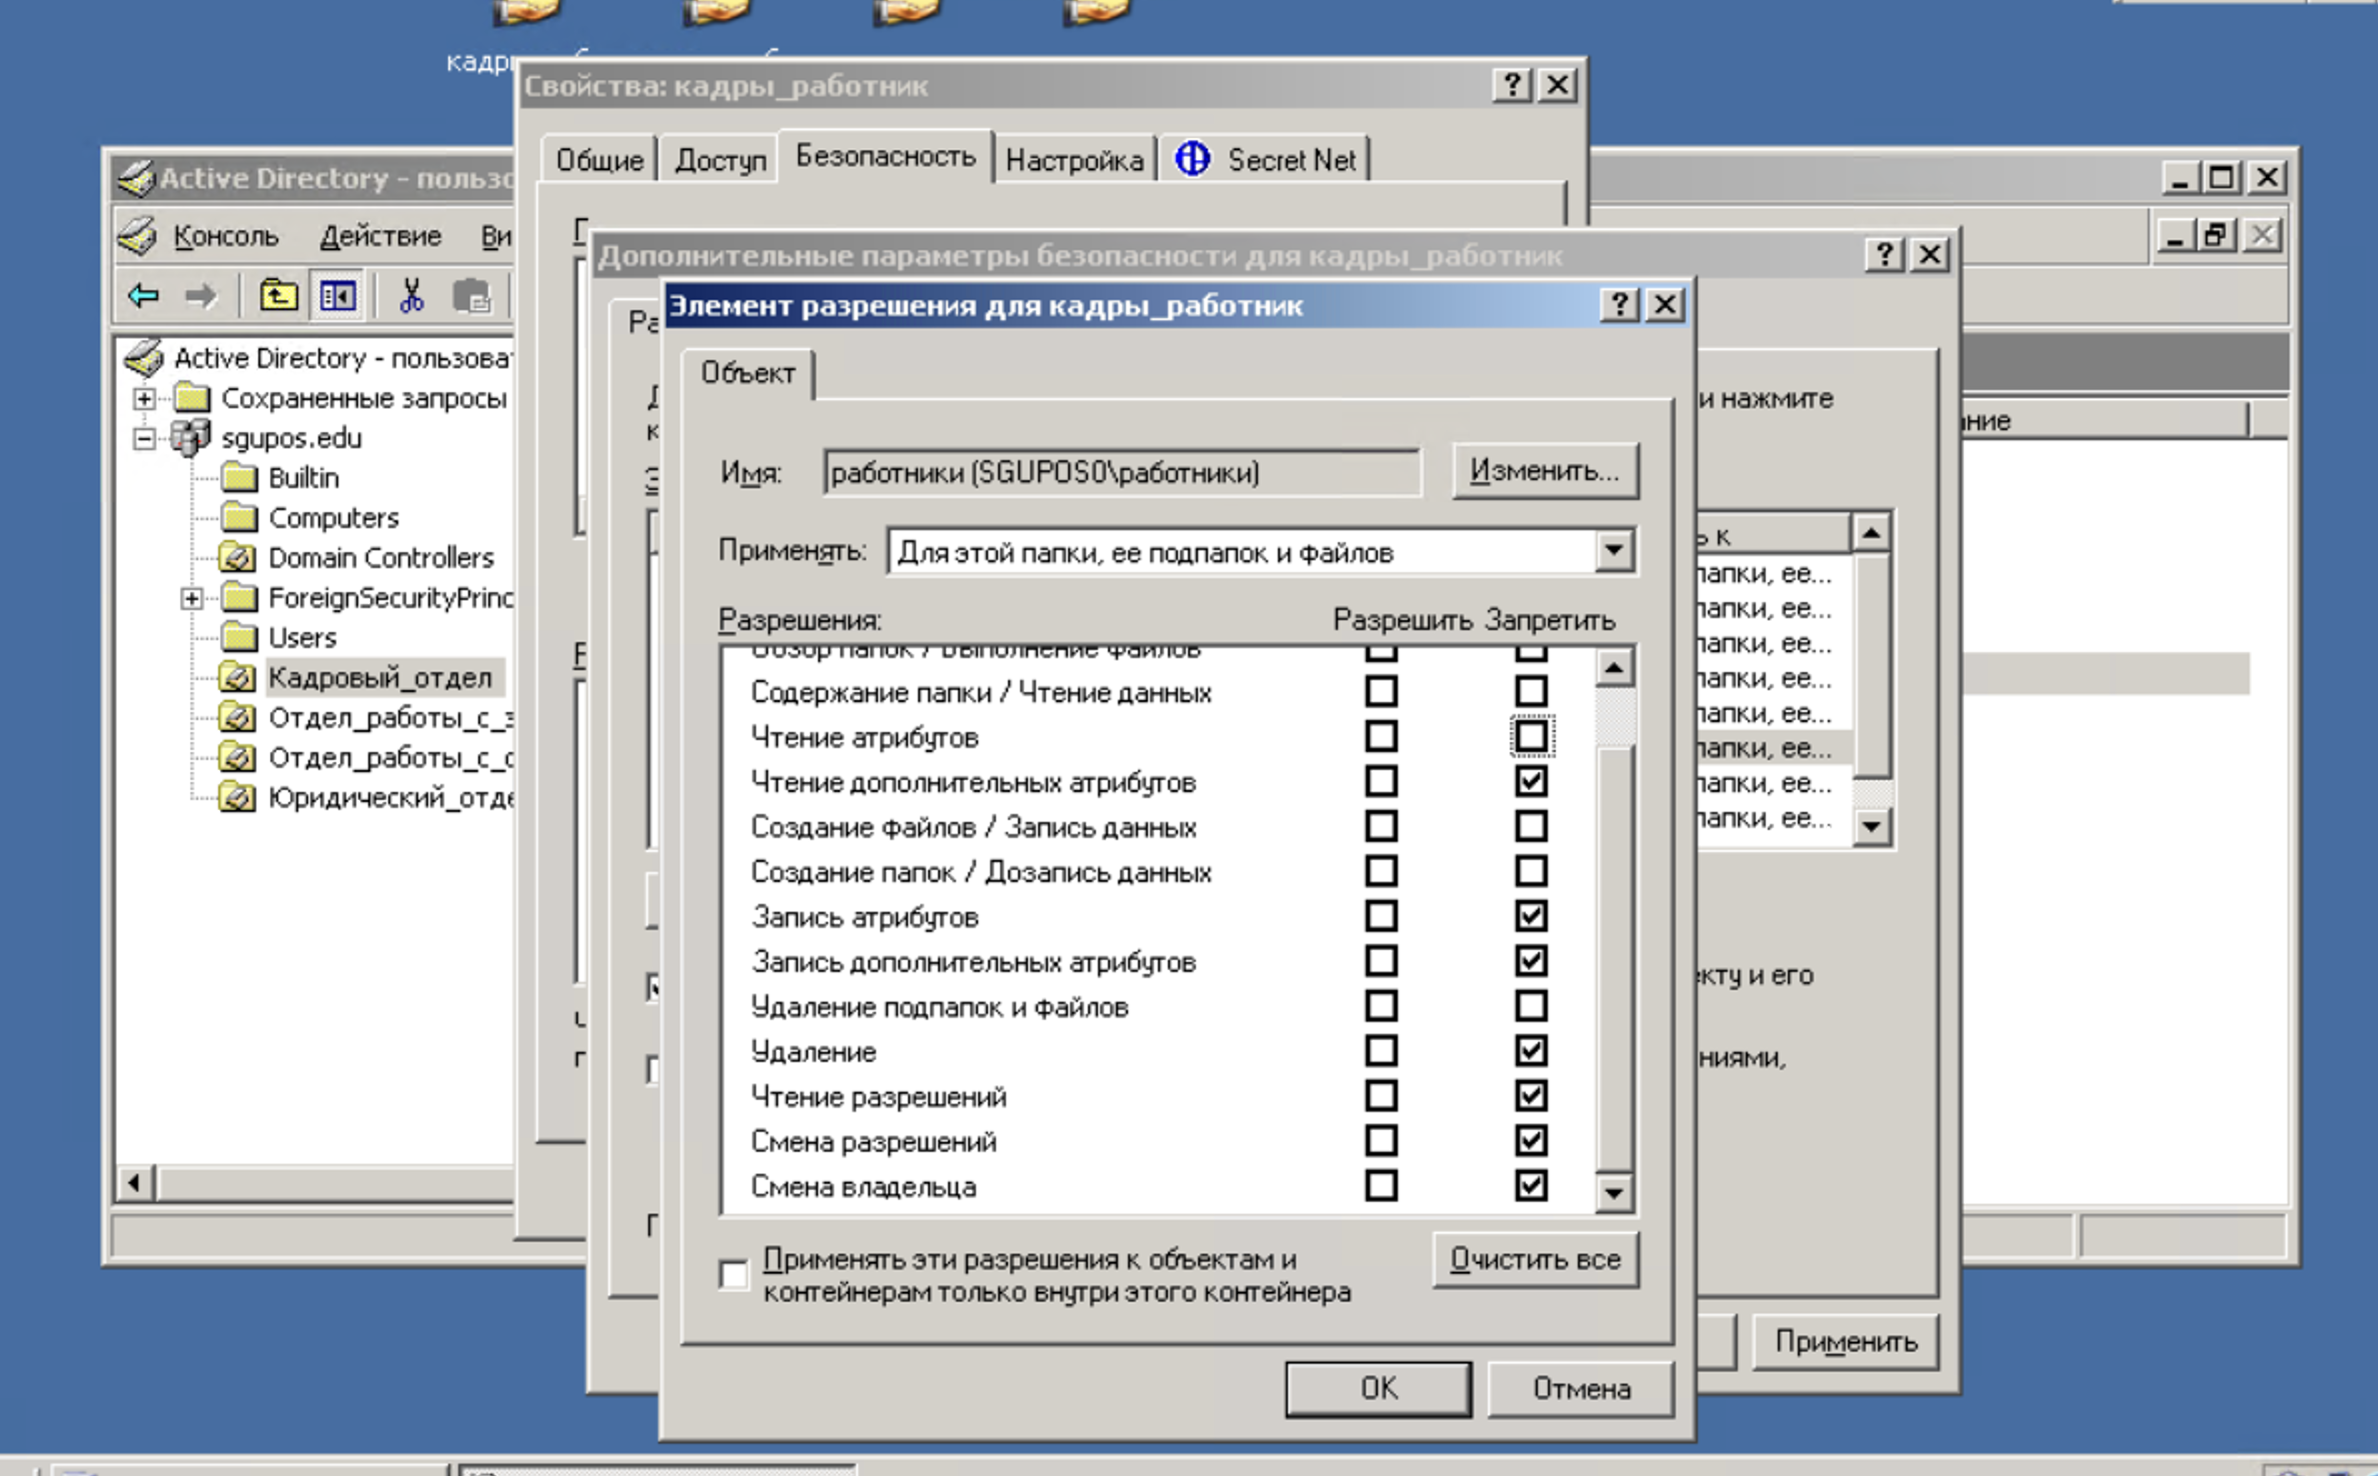
\includegraphics[width=0.9\textwidth]{pict/prac/61}
  \caption{Запрещено}
\end{figure}


Как мы видим полный доступ к папке имеет только администратор, он может менять владельца, права на доступ и т.д,
 что отвечает требованию к классу защищенности СВТ по ограничению прав для пользователей.
\begin{figure}[H]
    \centering
    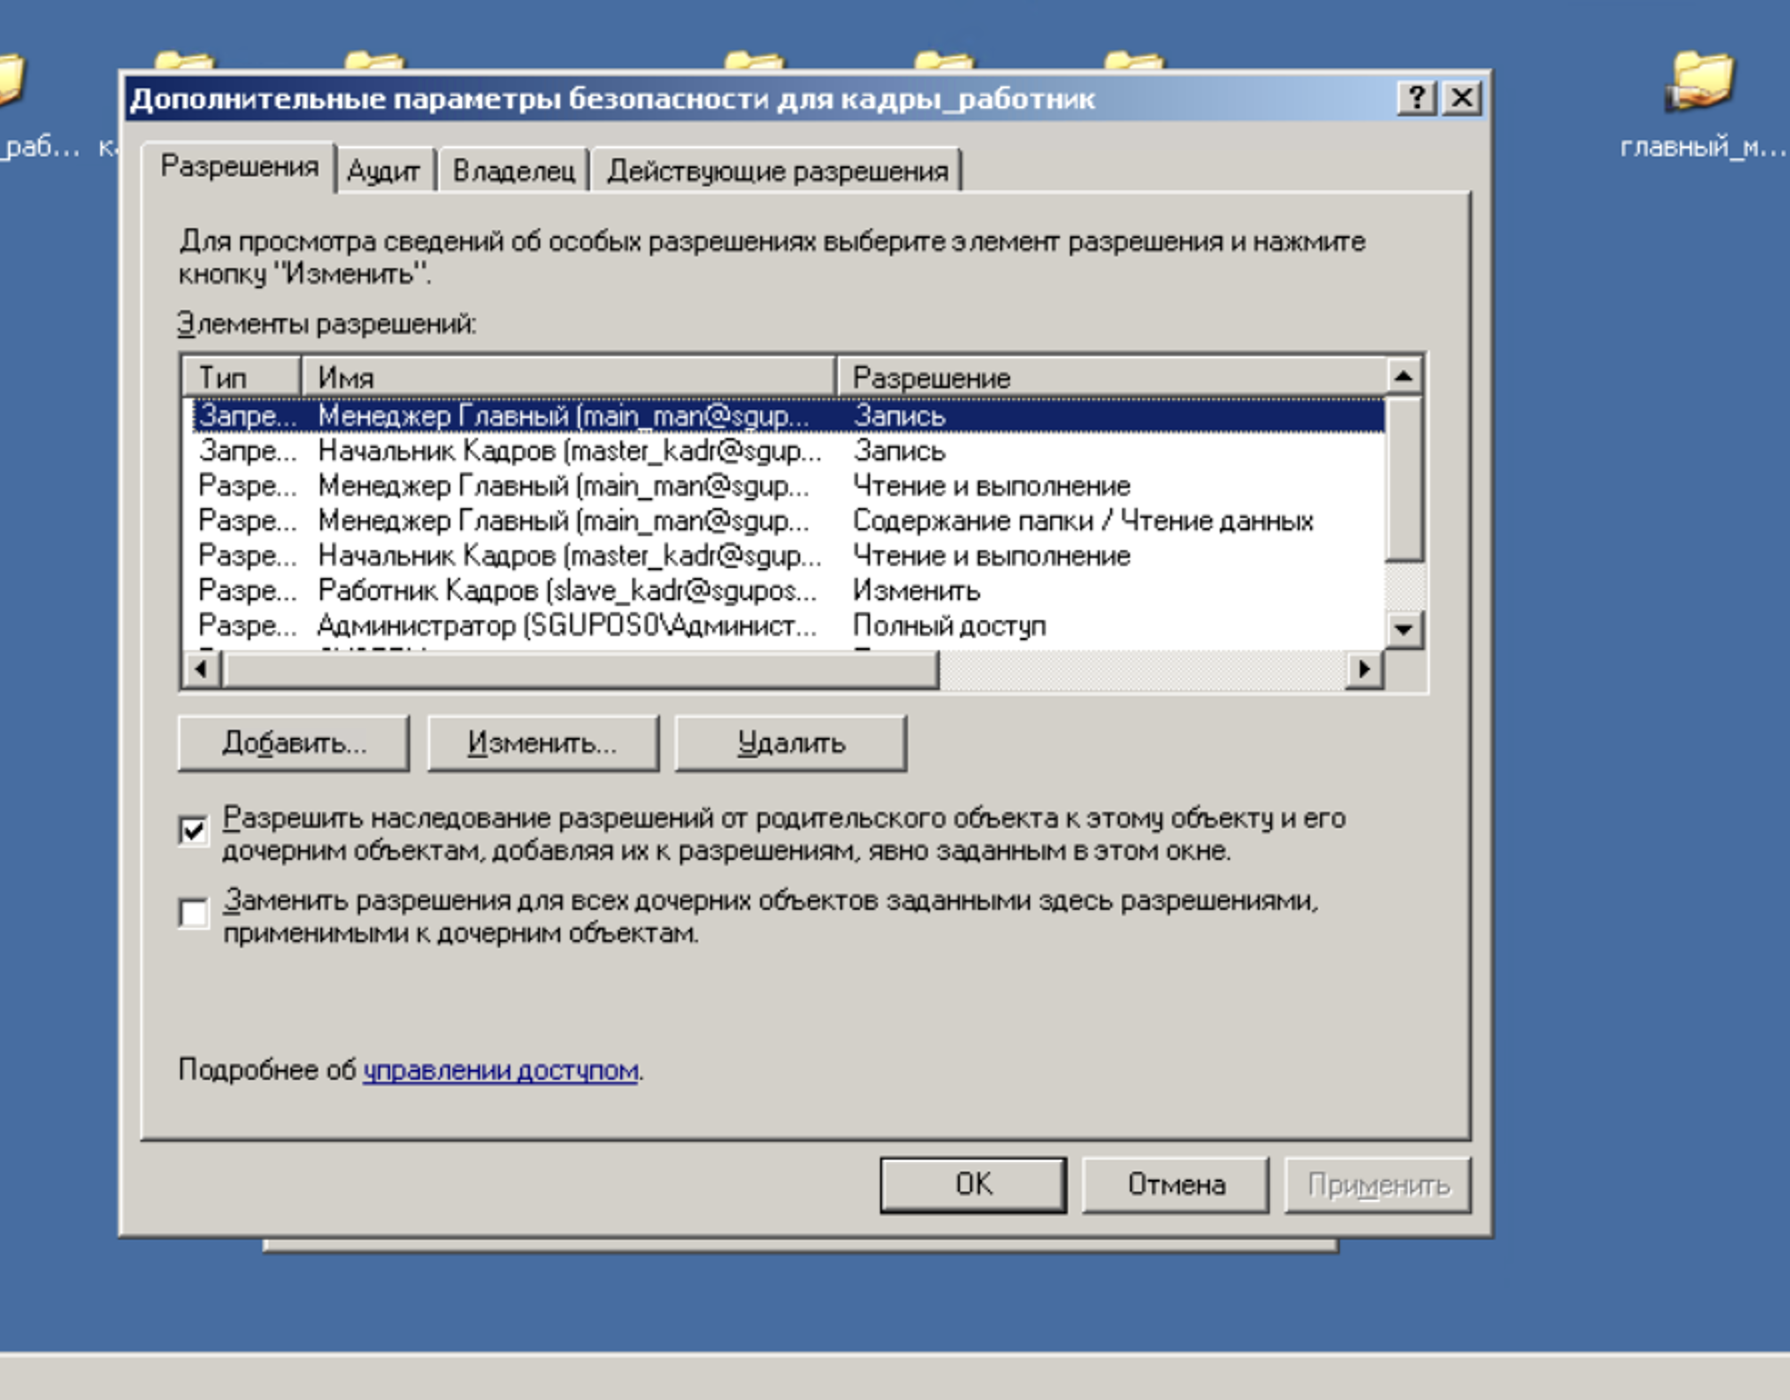
\includegraphics[width=1\textwidth]{pict/prac/9}
    \caption{Права на папку сотрудника}
    \label{fig:21}
\end{figure}

\begin{figure}[H]
  \centering
  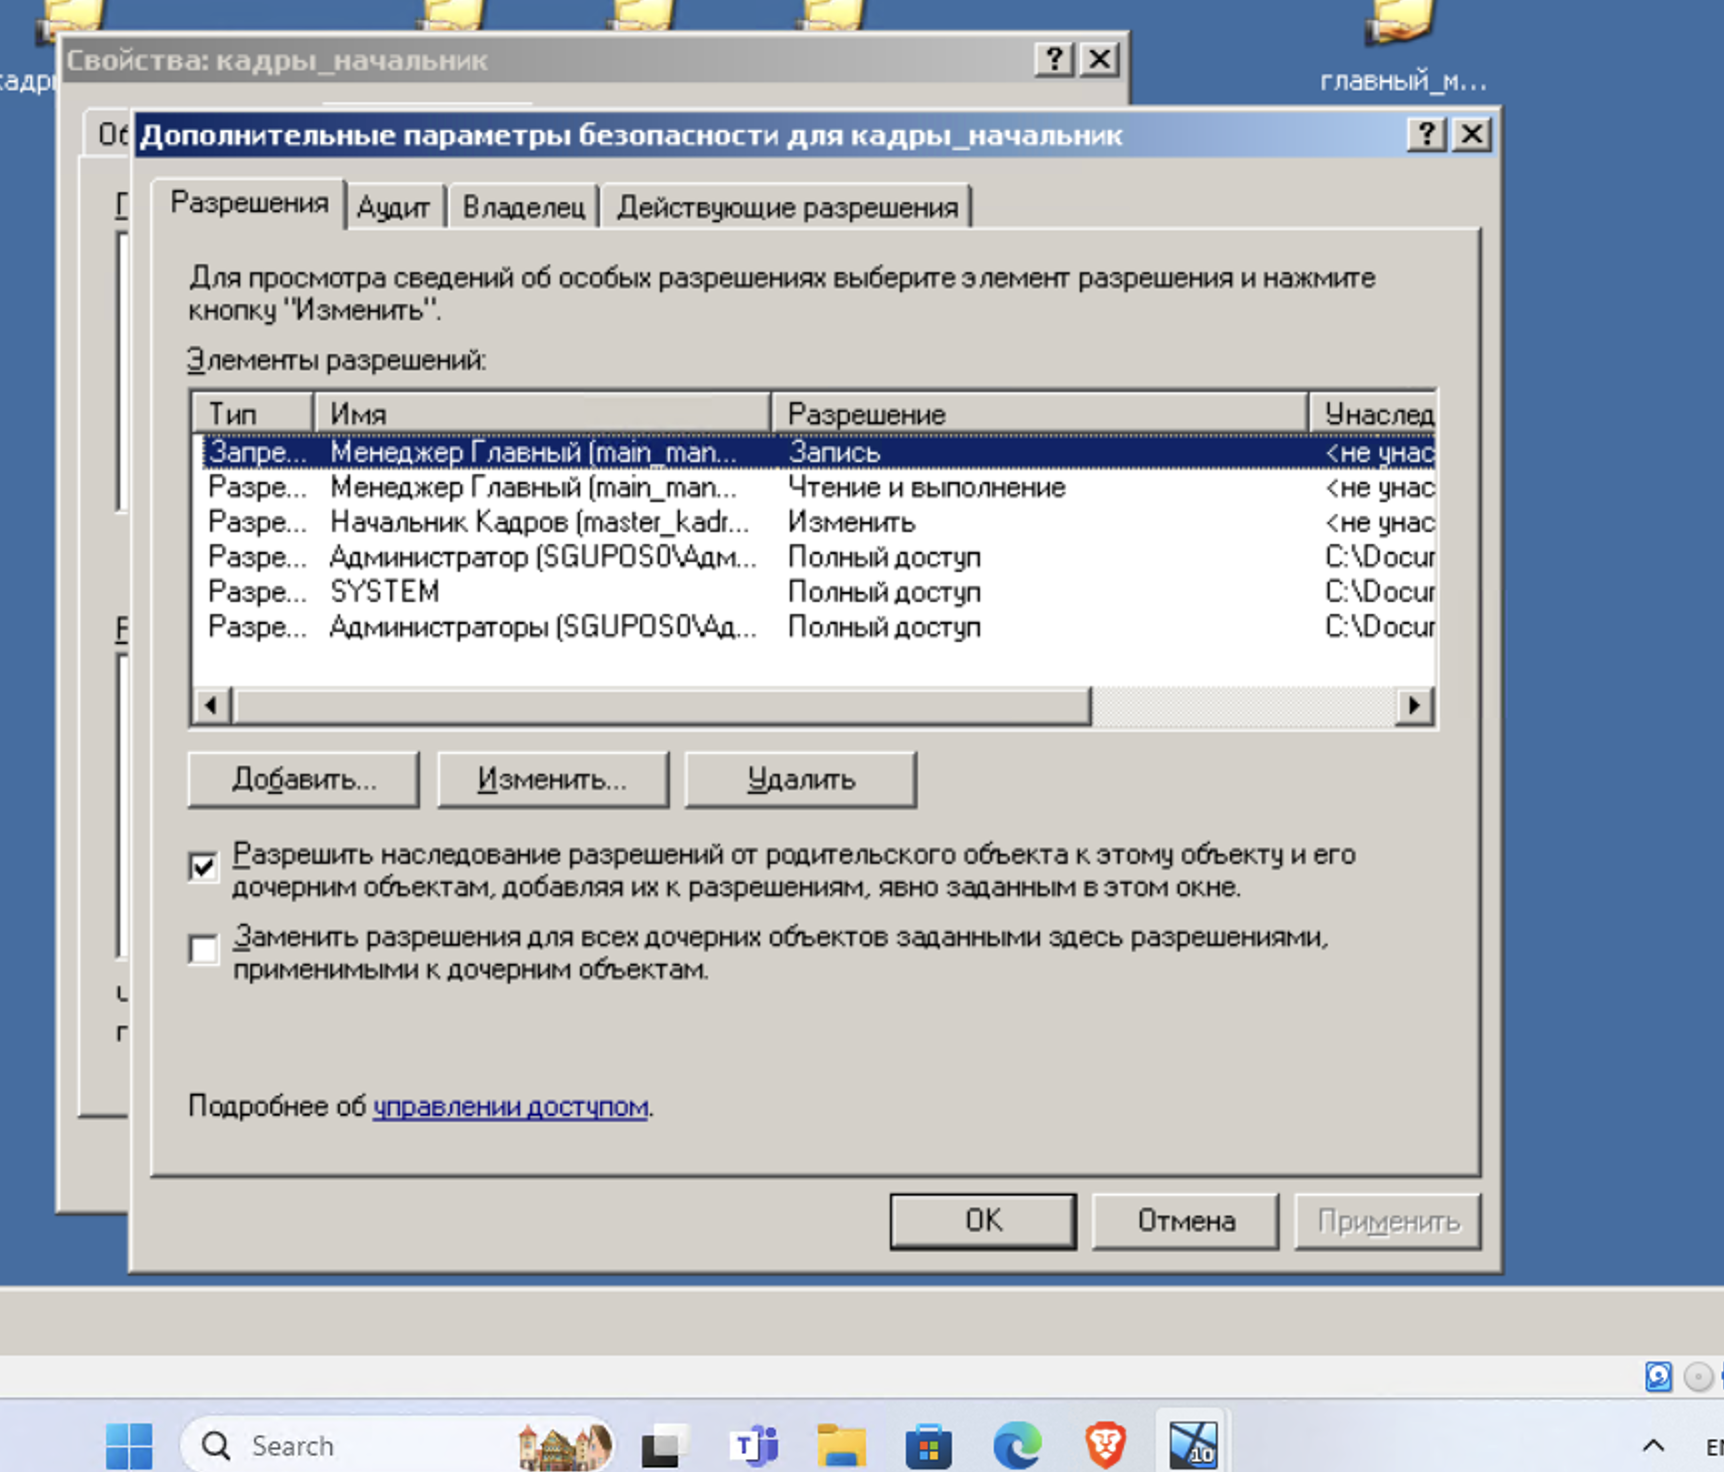
\includegraphics[width=1\textwidth]{pict/prac/10}
  \caption{Права на папку начальника}
  \label{fig:22}
\end{figure}

\newpage
К папке главного менеджера доступ и права имеет только сам менеджер.
\begin{figure}[H]
  \centering
  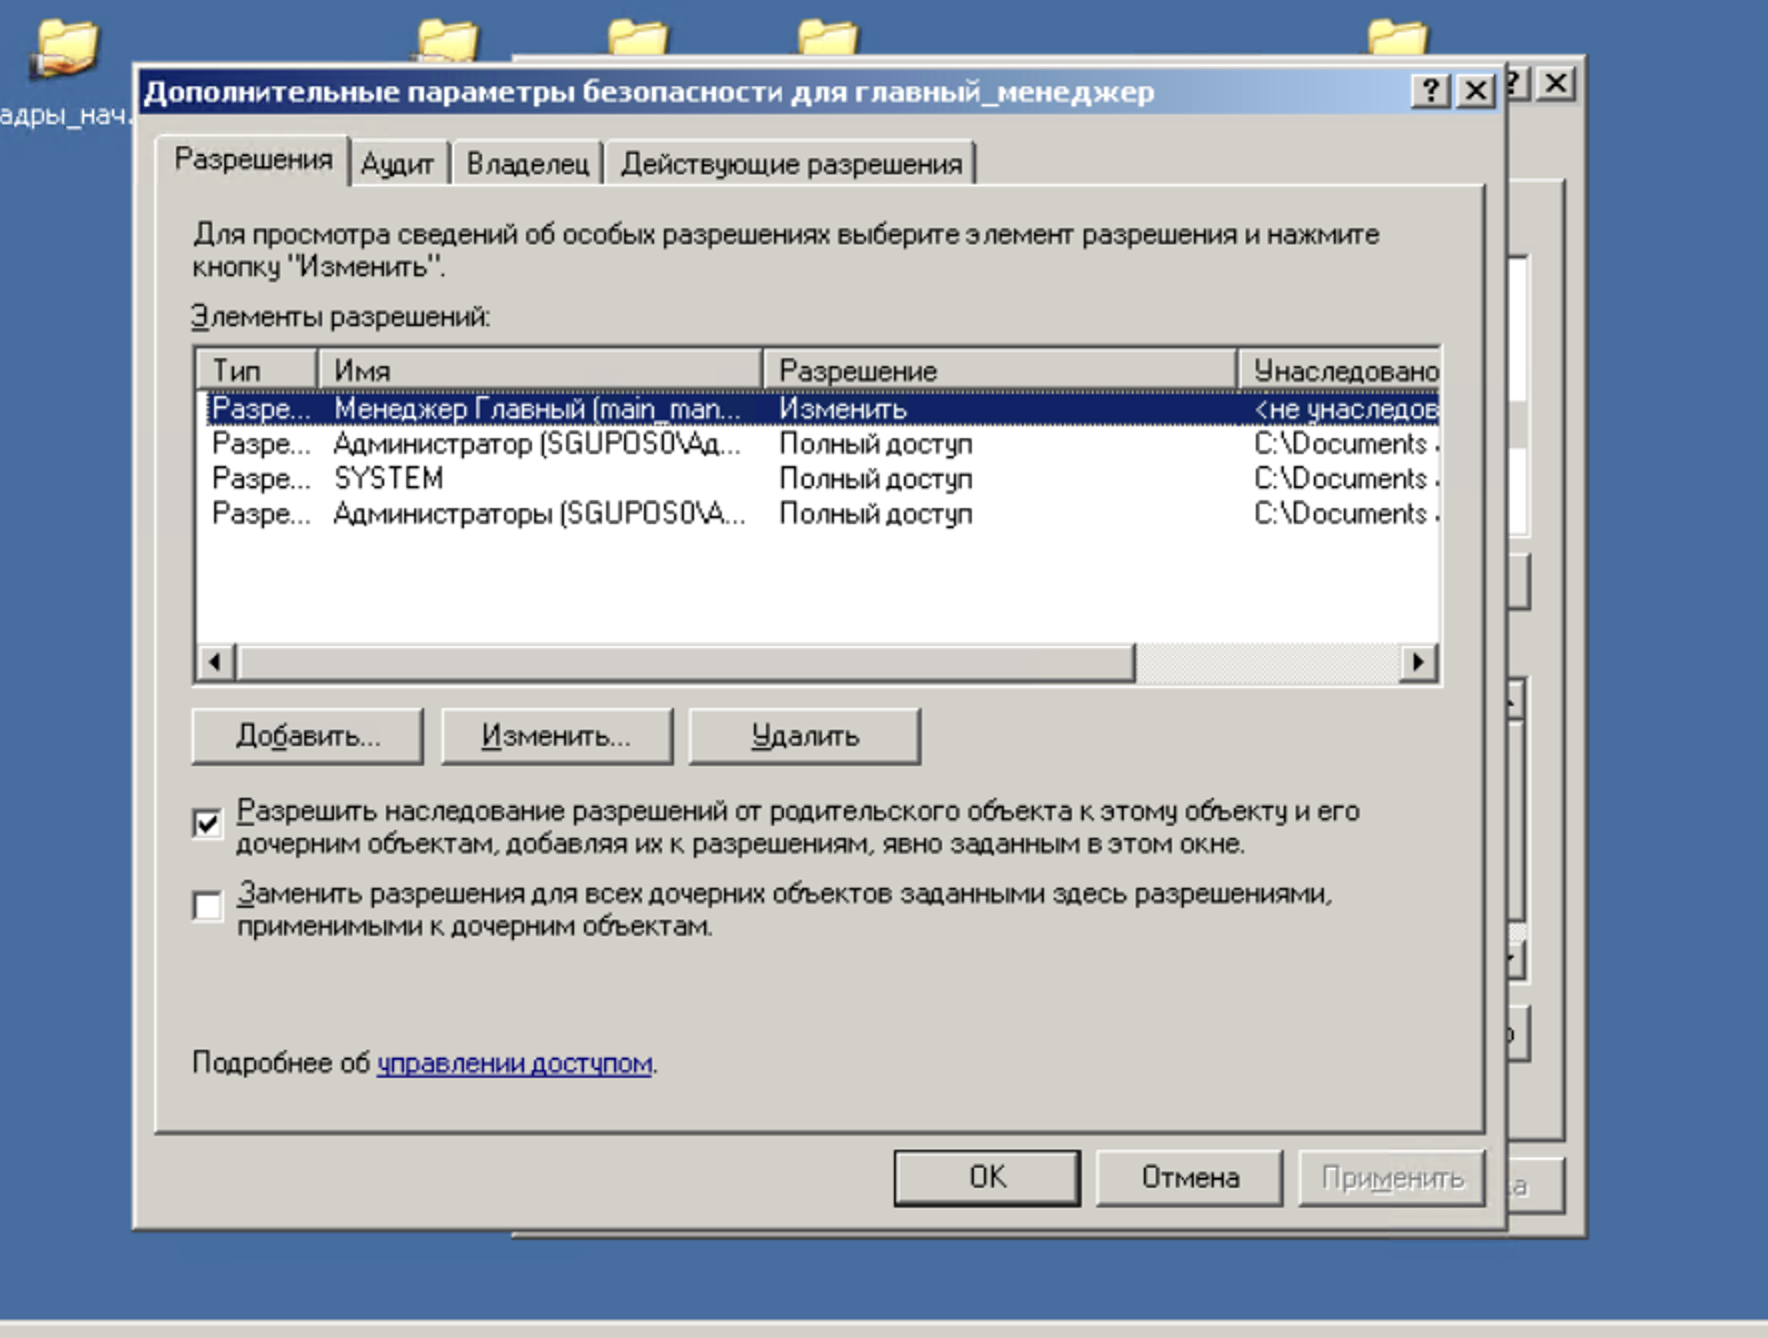
\includegraphics[width=1\textwidth]{pict/prac/11}
  \caption{Права на папку главного менеджера}
  \label{fig:48}
\end{figure}
Настроем аналогичные правила для аккаунтов всех остальных подразделений.

\newpage


\subsubsection{Проверка работы настроек}

Зайдем в учетную запись работника кадров, проверим доступность.
\begin{figure}[H]
  \centering
  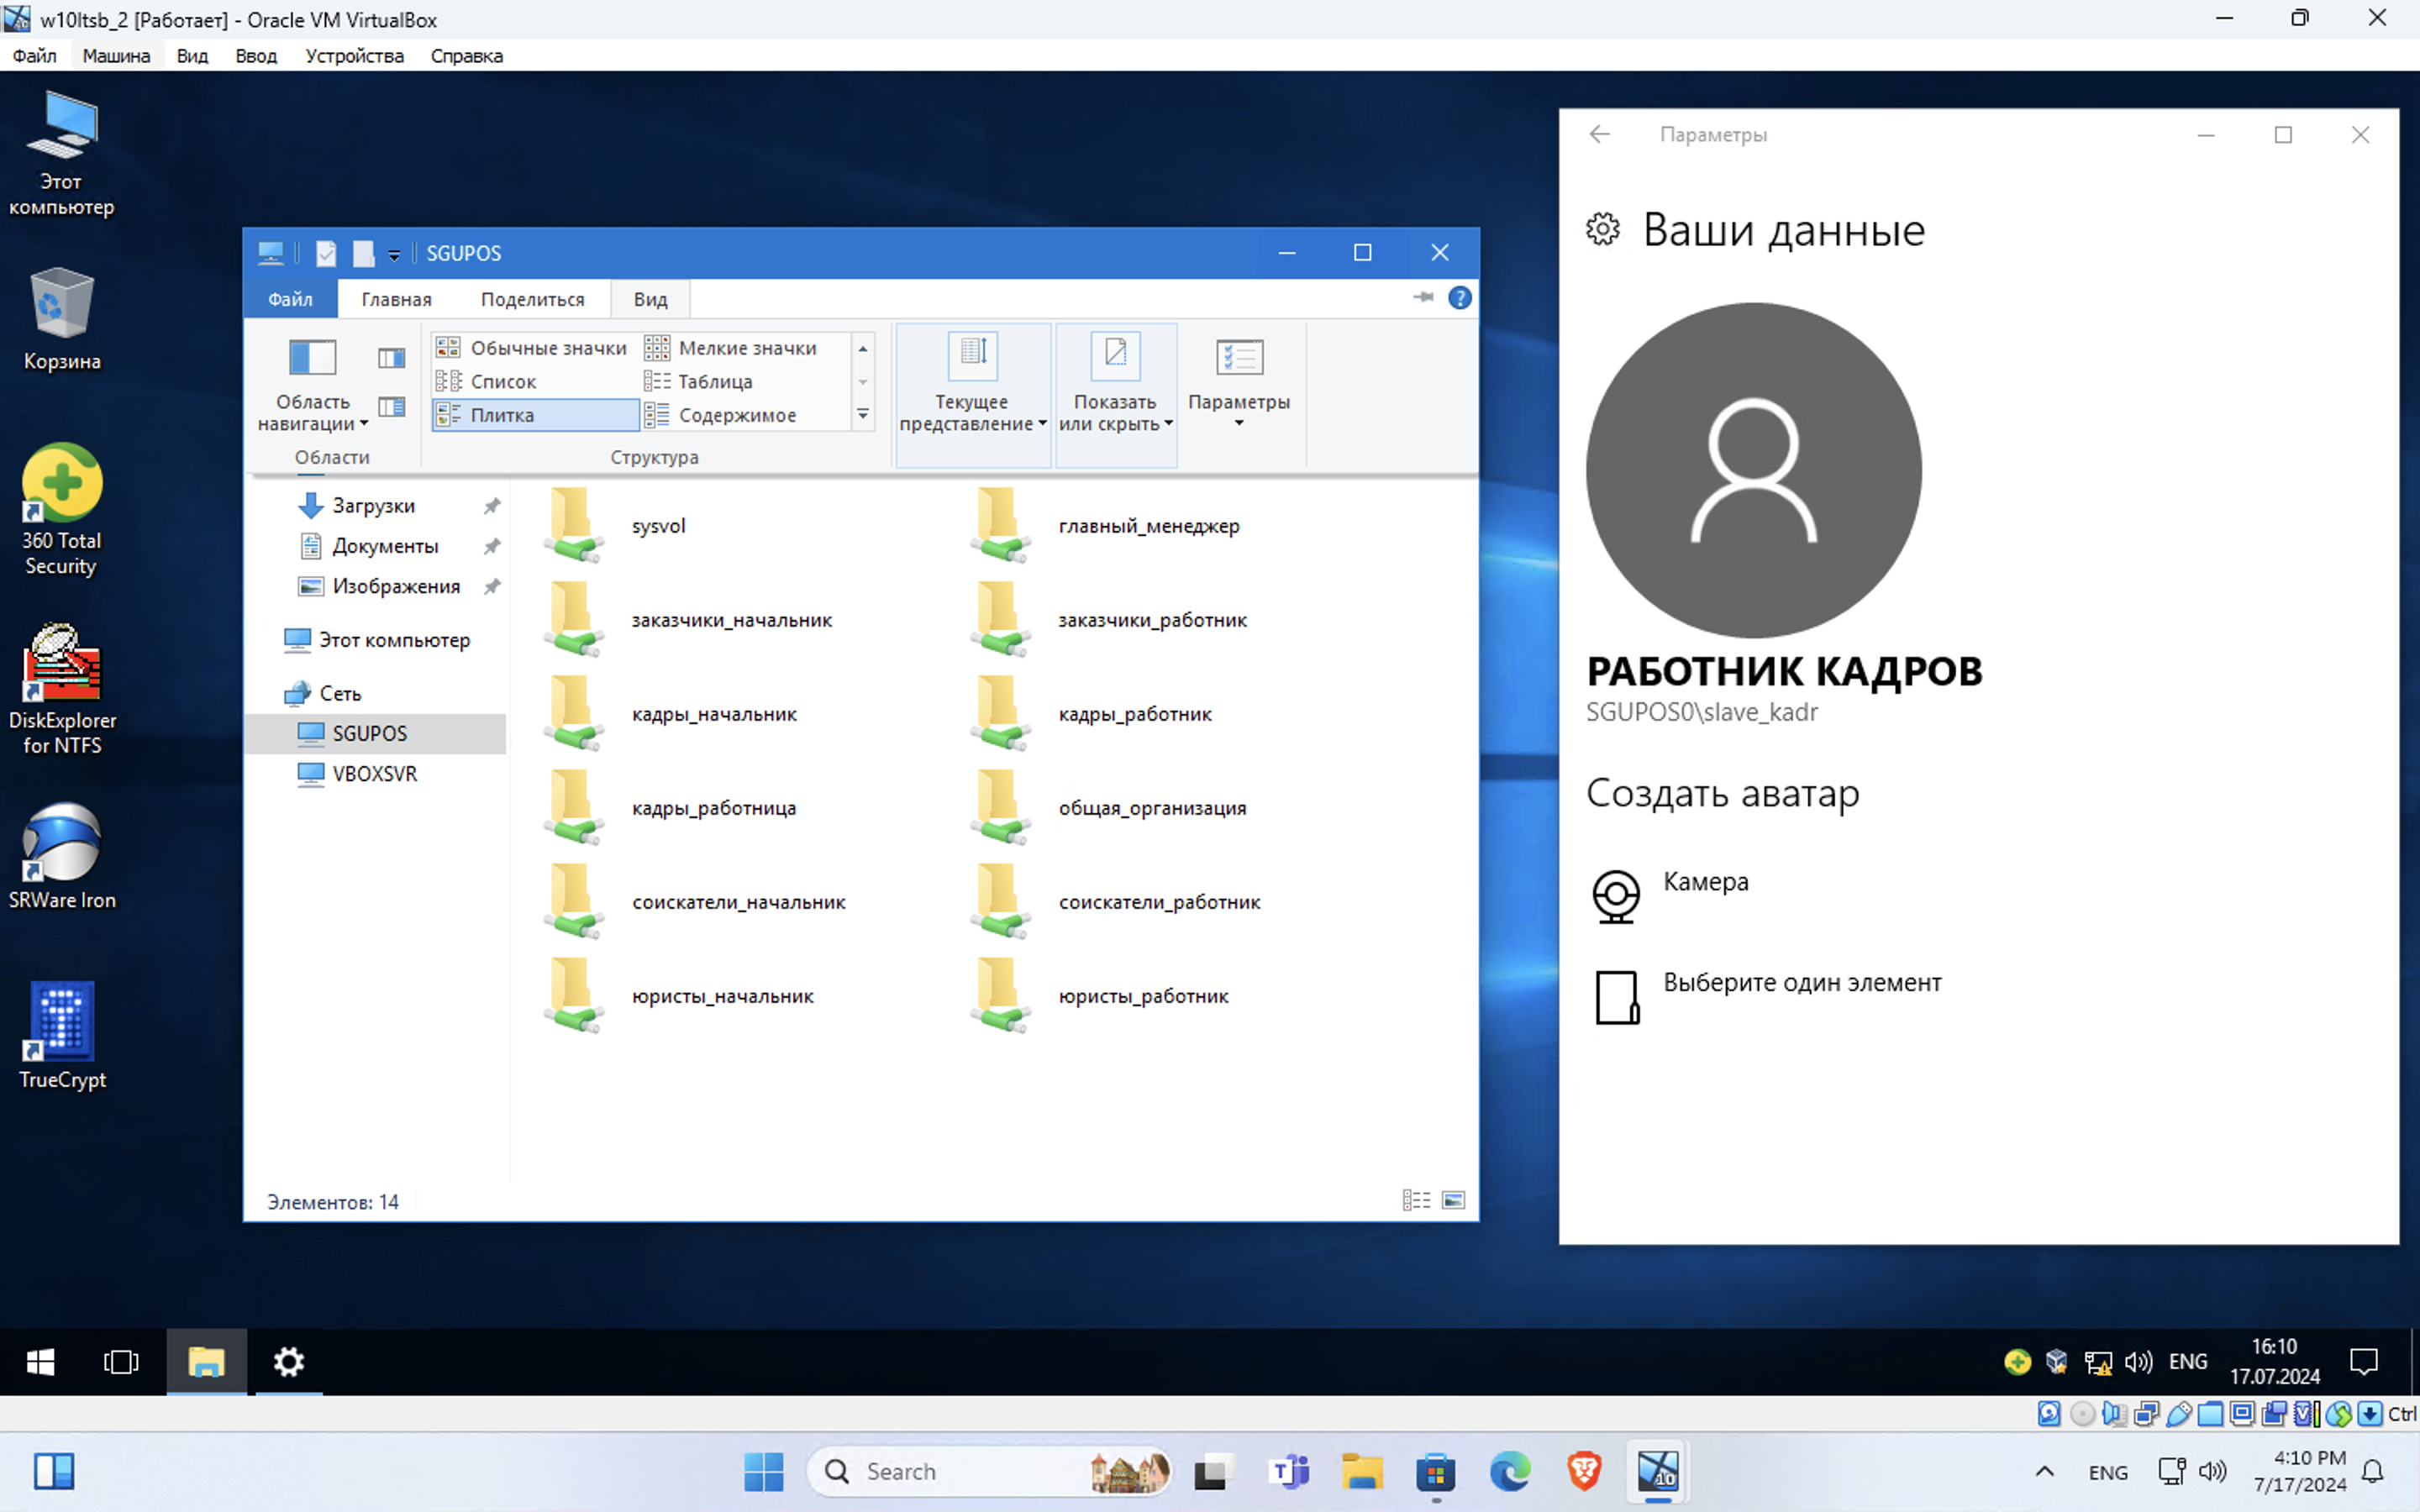
\includegraphics[width=0.9\textwidth]{pict/prac/25}
  \caption{Аккаунт работника кадров}
  \label{fig:24}
\end{figure}

\begin{figure}[H]
  \centering
  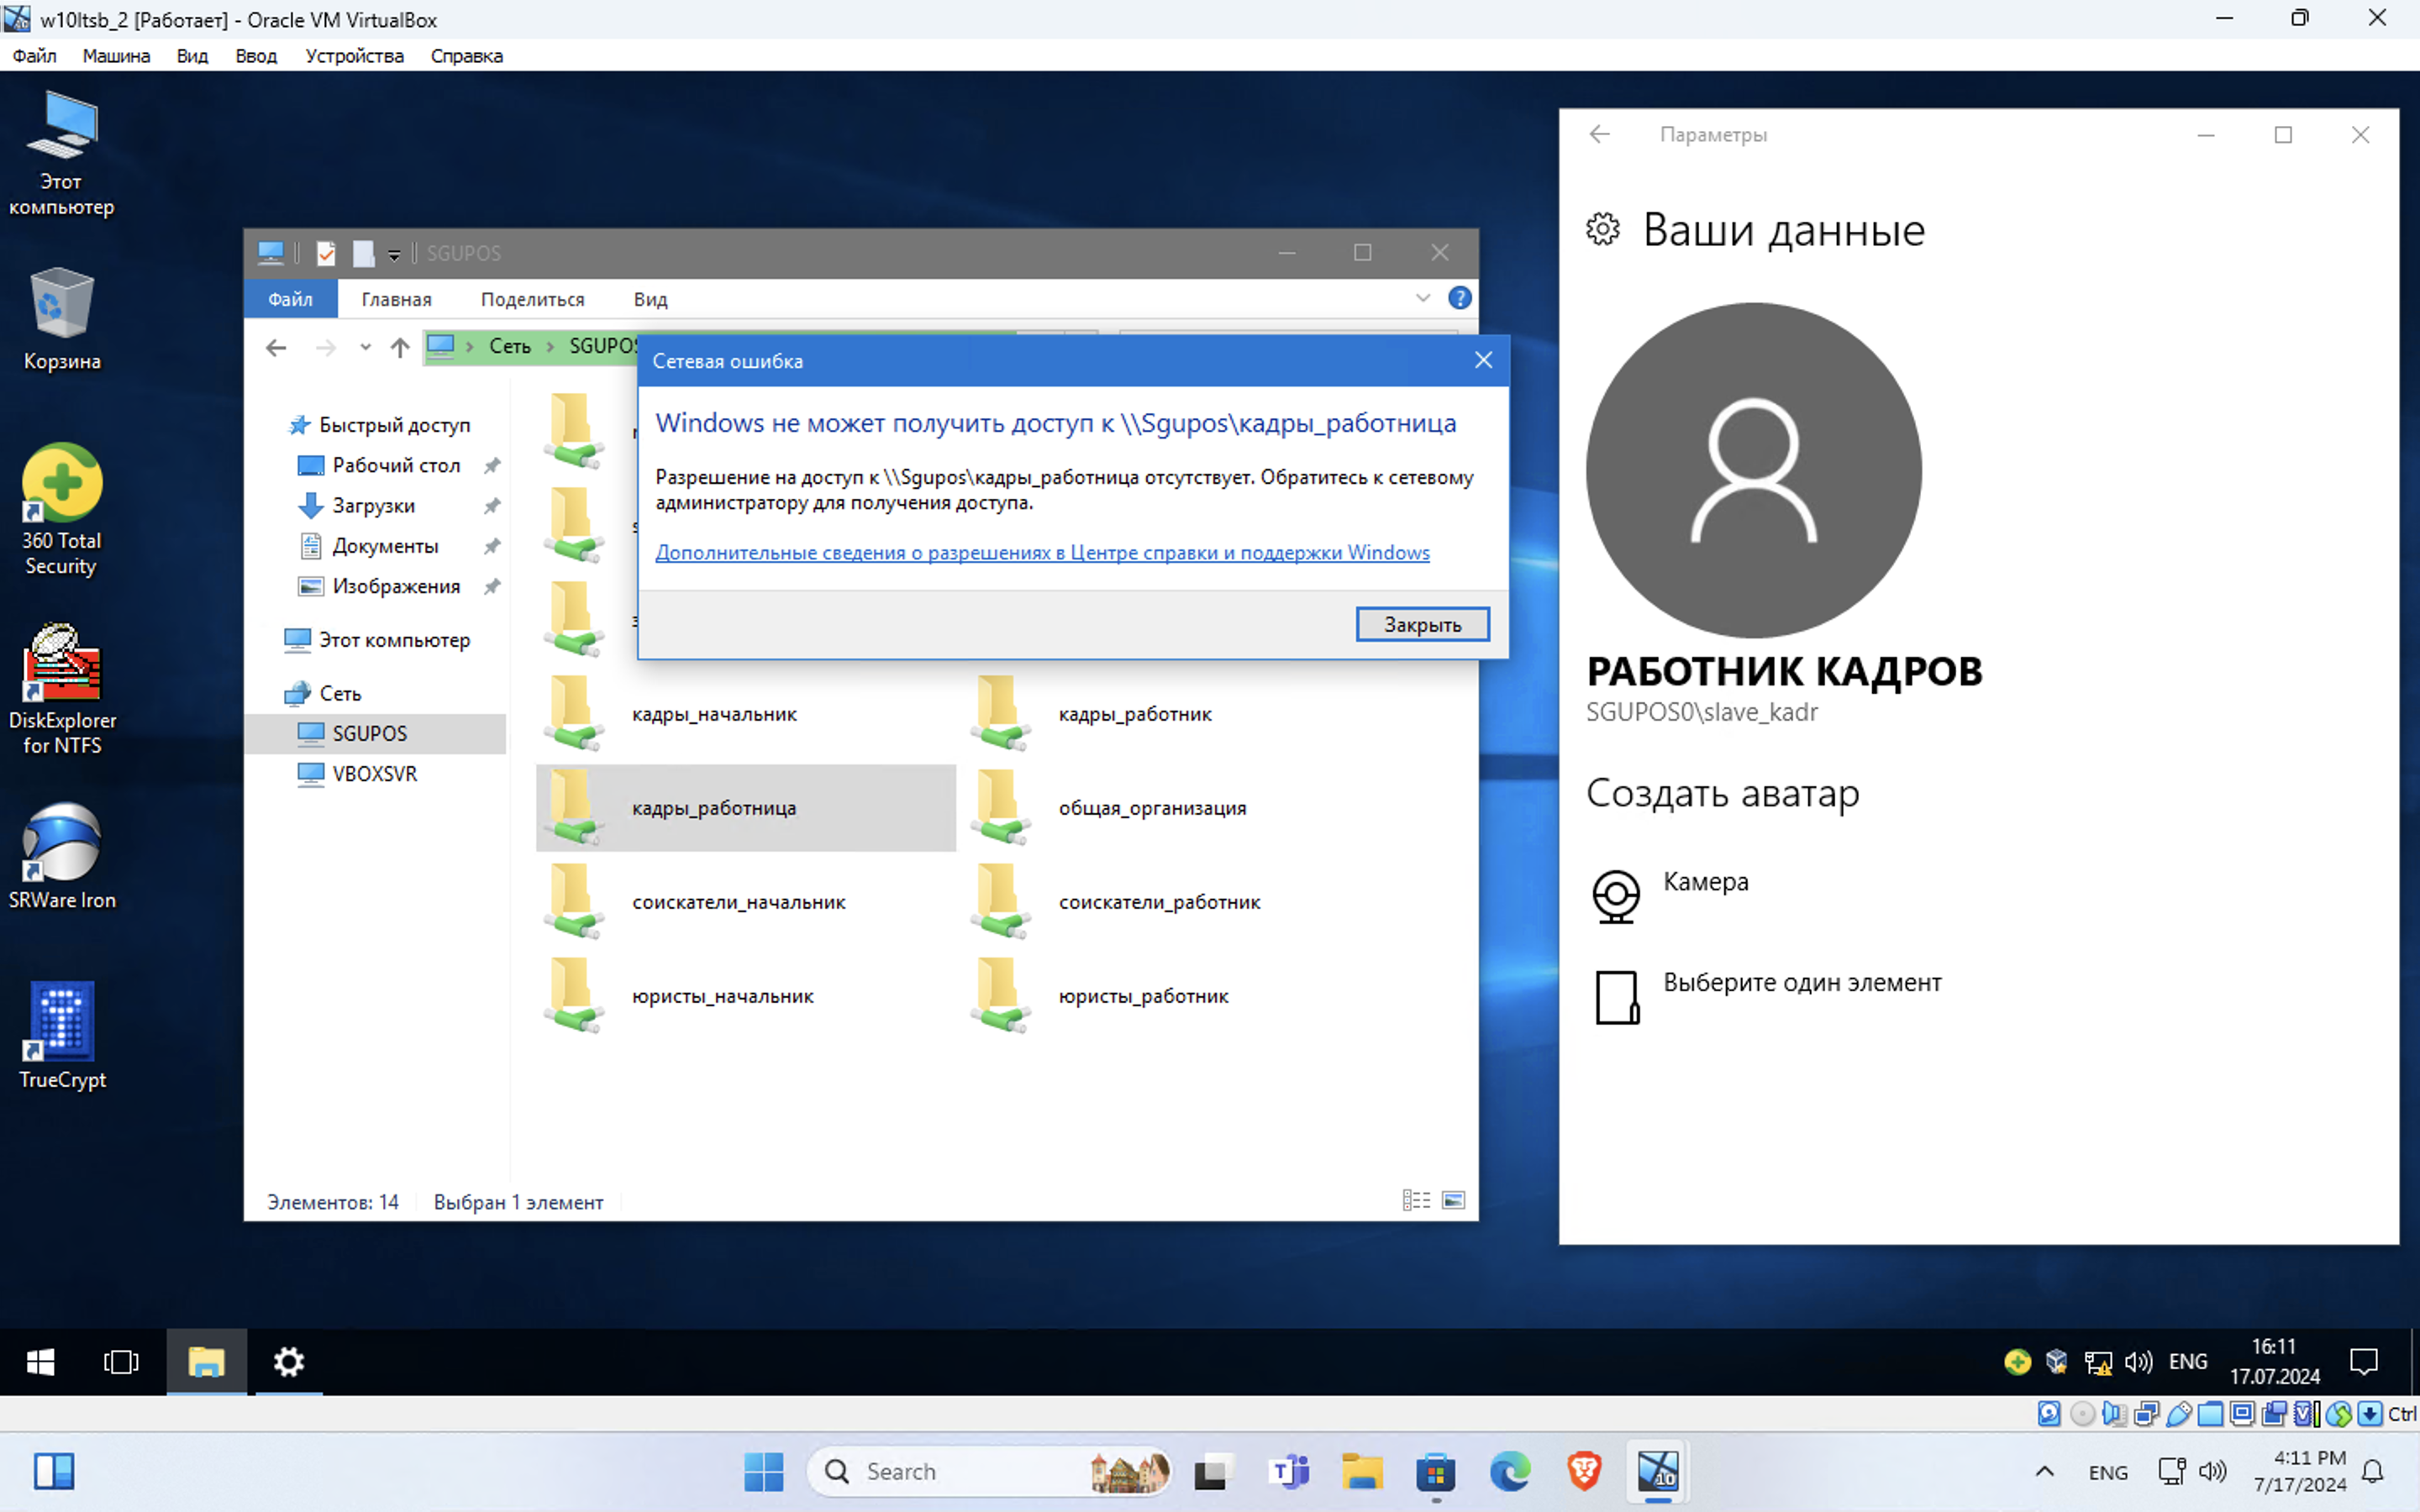
\includegraphics[width=0.9\textwidth]{pict/prac/26}
  \caption{Работник кадров -> Работница кадров}
  \label{fig:25}
\end{figure}


\begin{figure}[H]
  \centering
  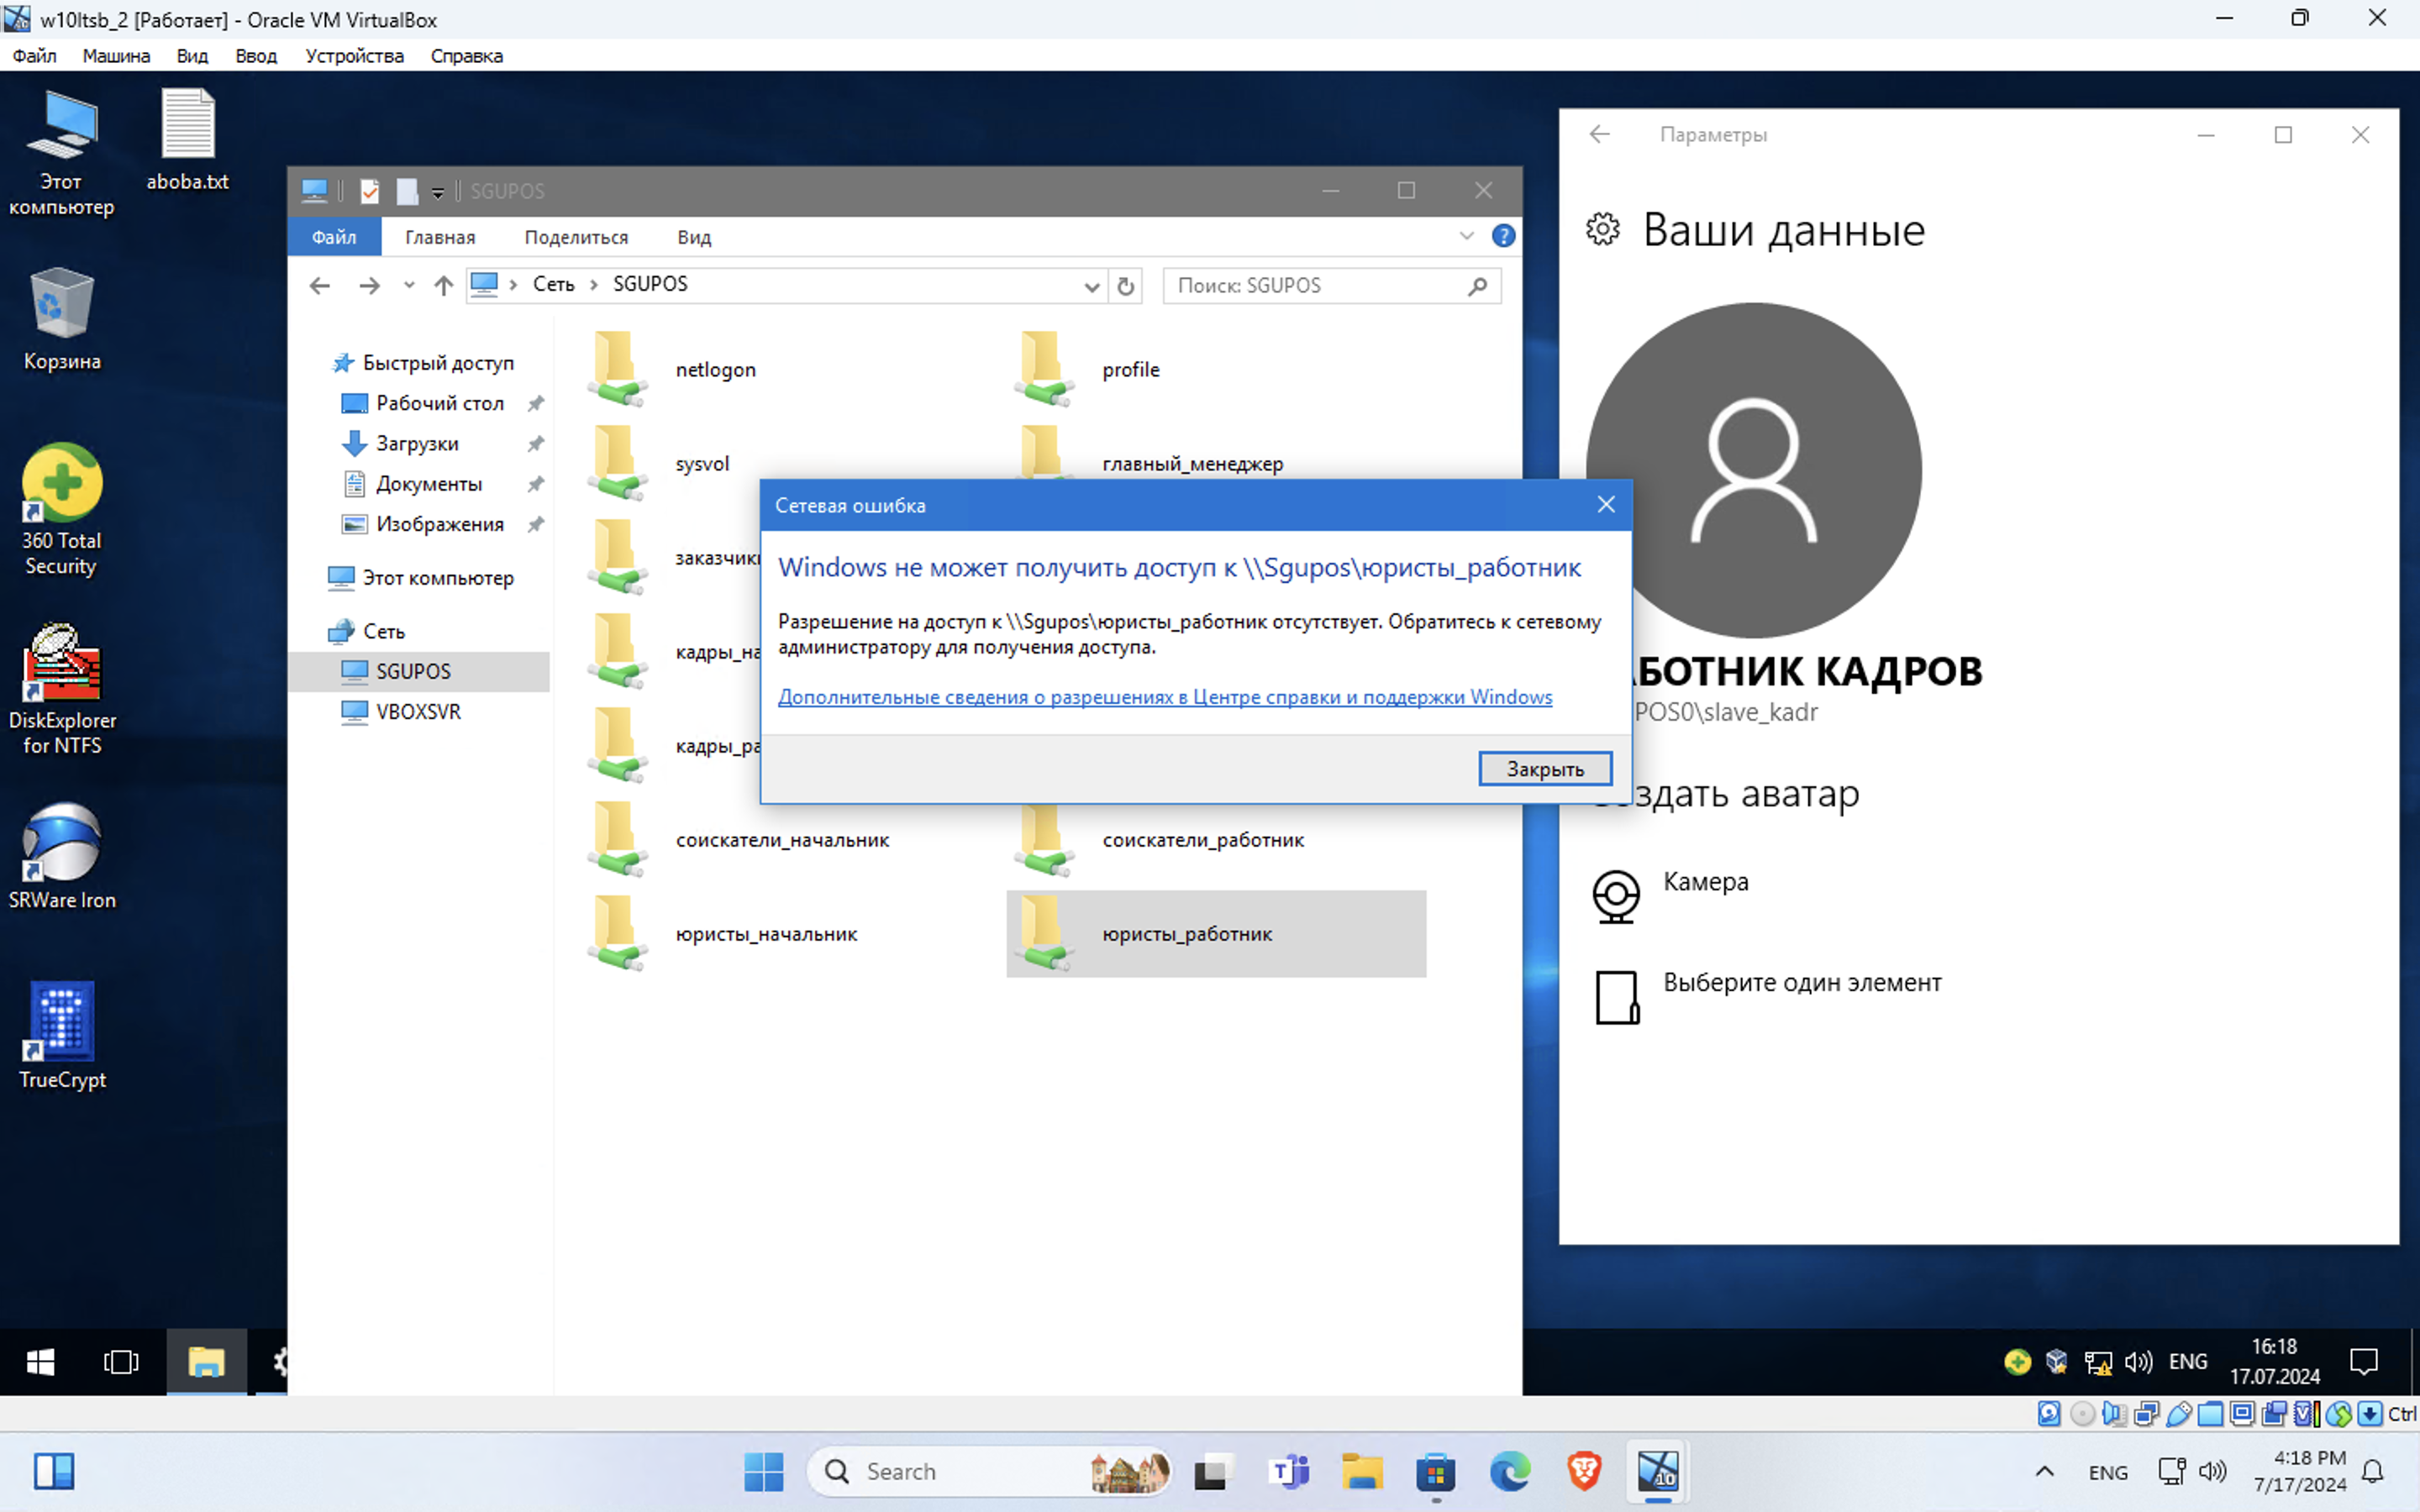
\includegraphics[width=1\textwidth]{pict/prac/32}
  \caption{Работник кадров -> Работник юристов}
  \label{fig:31}
\end{figure}


\begin{figure}[H]
  \centering
  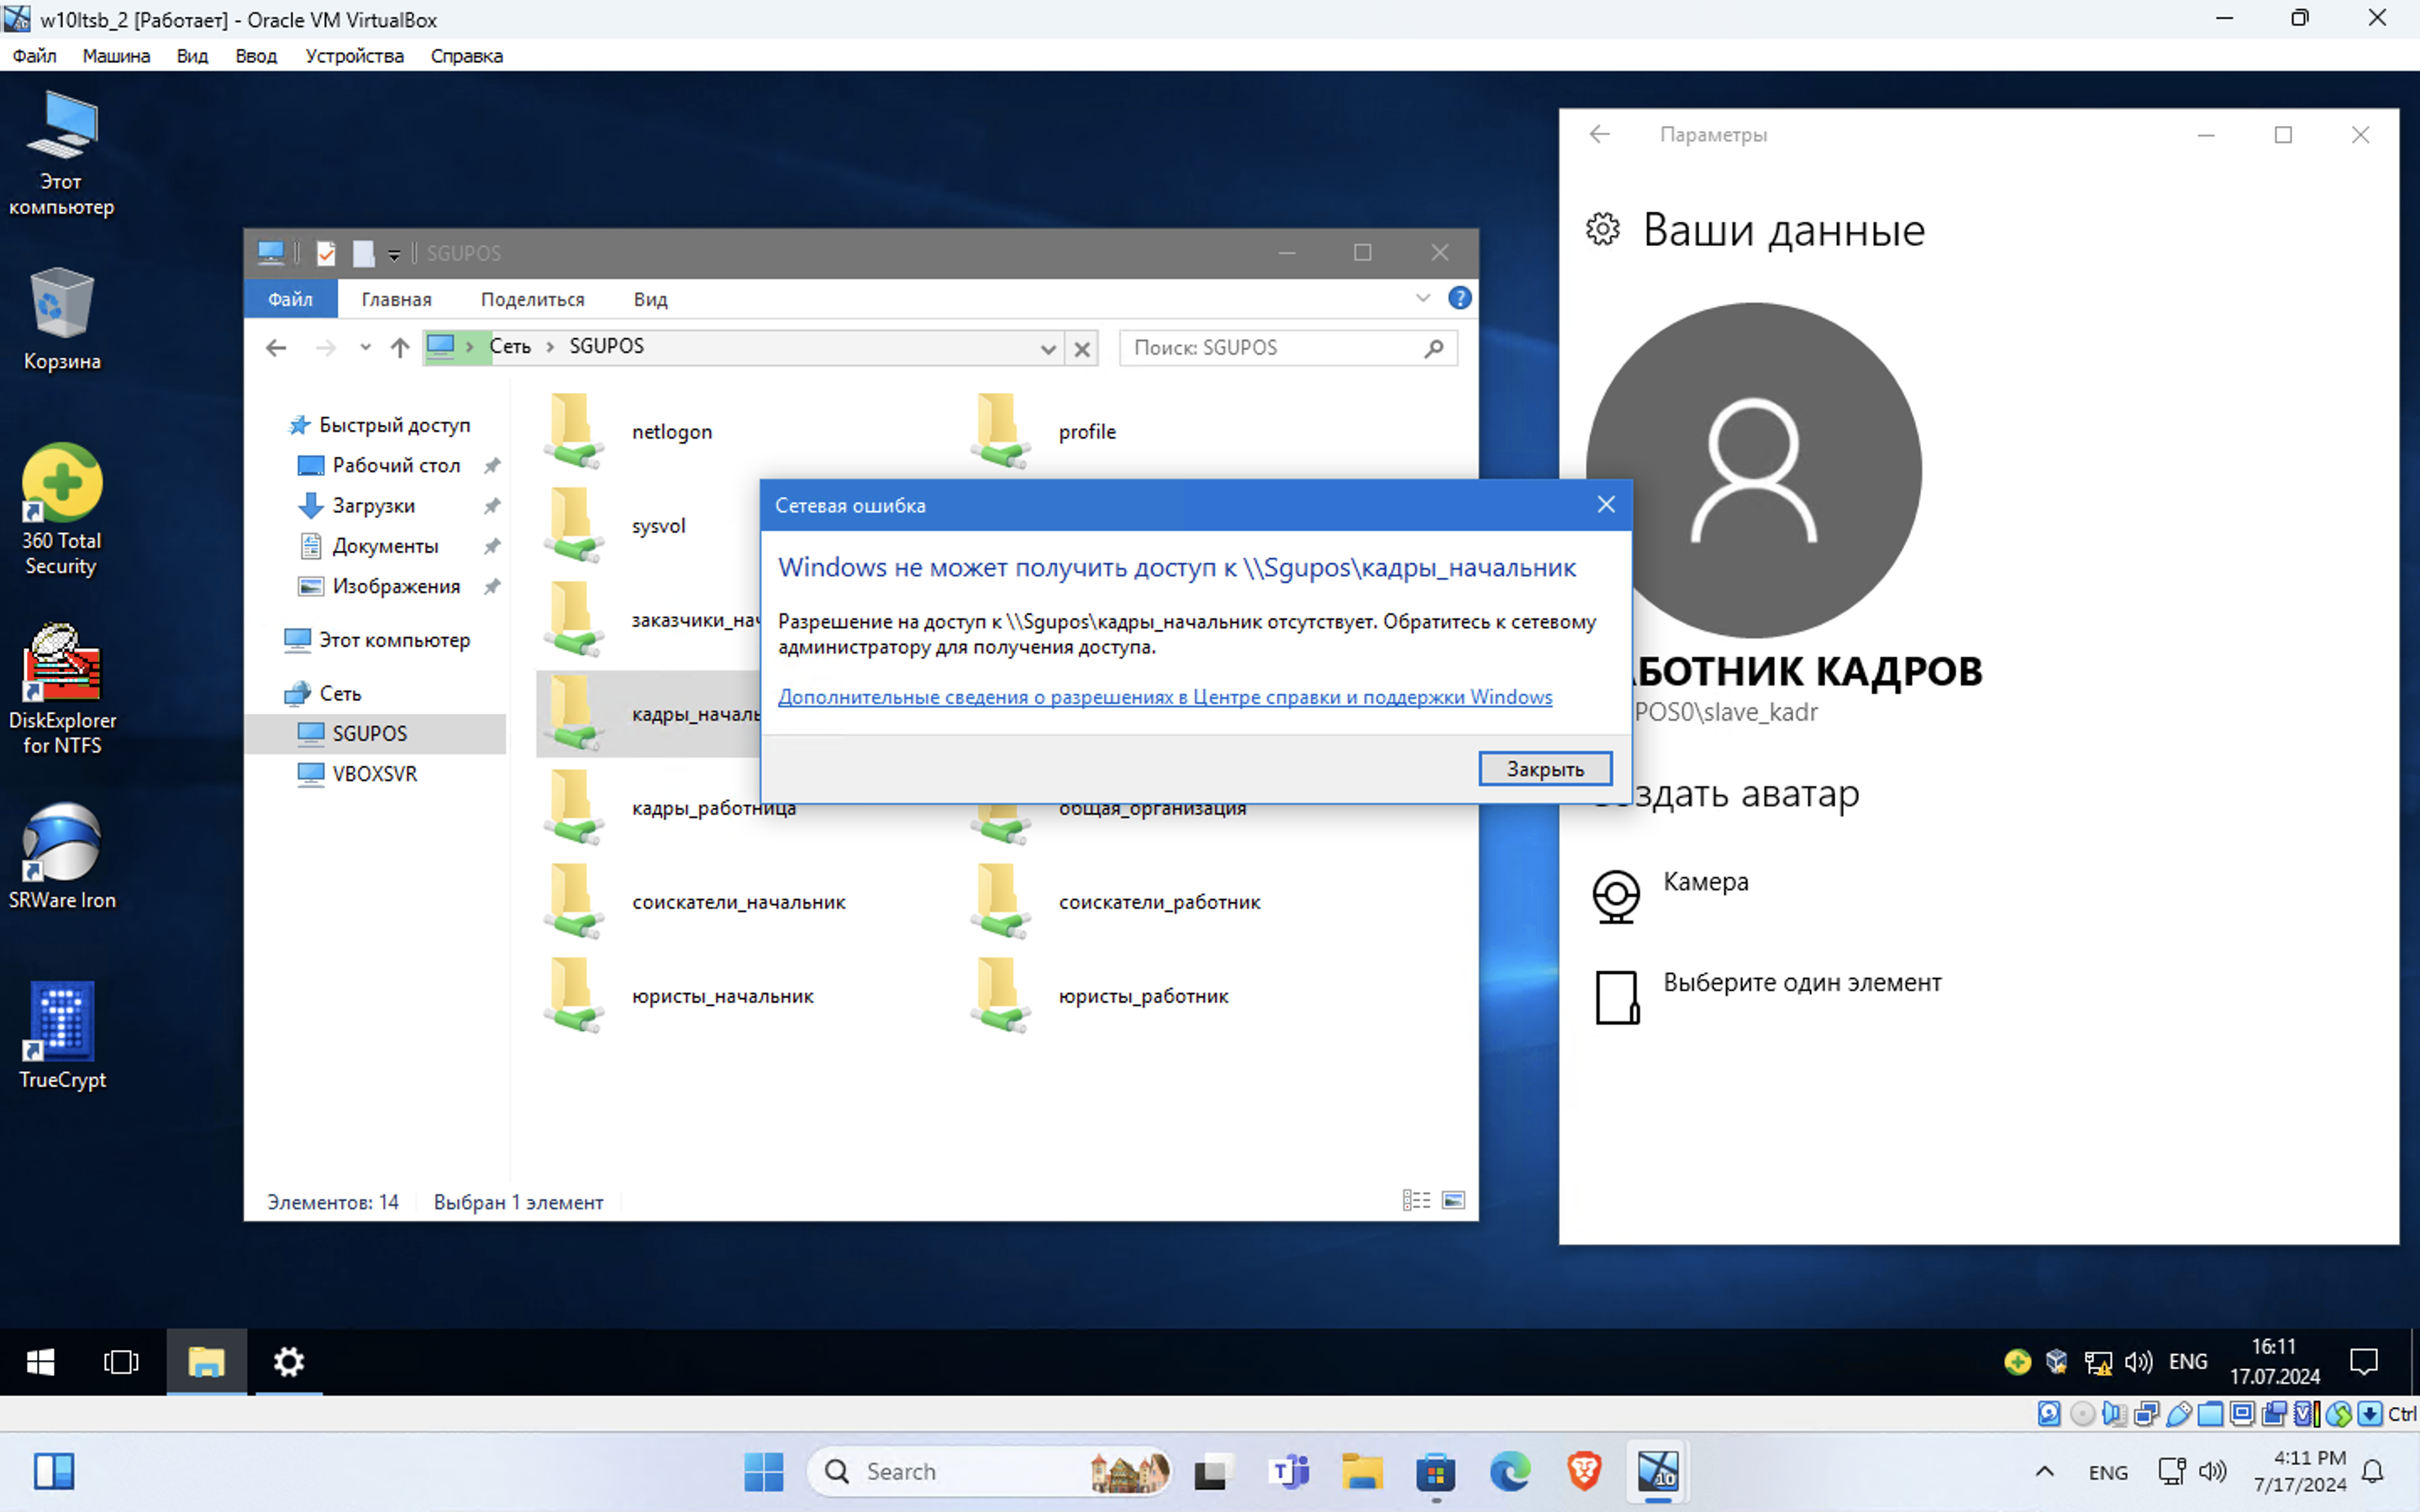
\includegraphics[width=1\textwidth]{pict/prac/27}
  \caption{Работник кадров -> Начальник кадров}
  \label{fig:26}
\end{figure}


\begin{figure}[H]
  \centering
  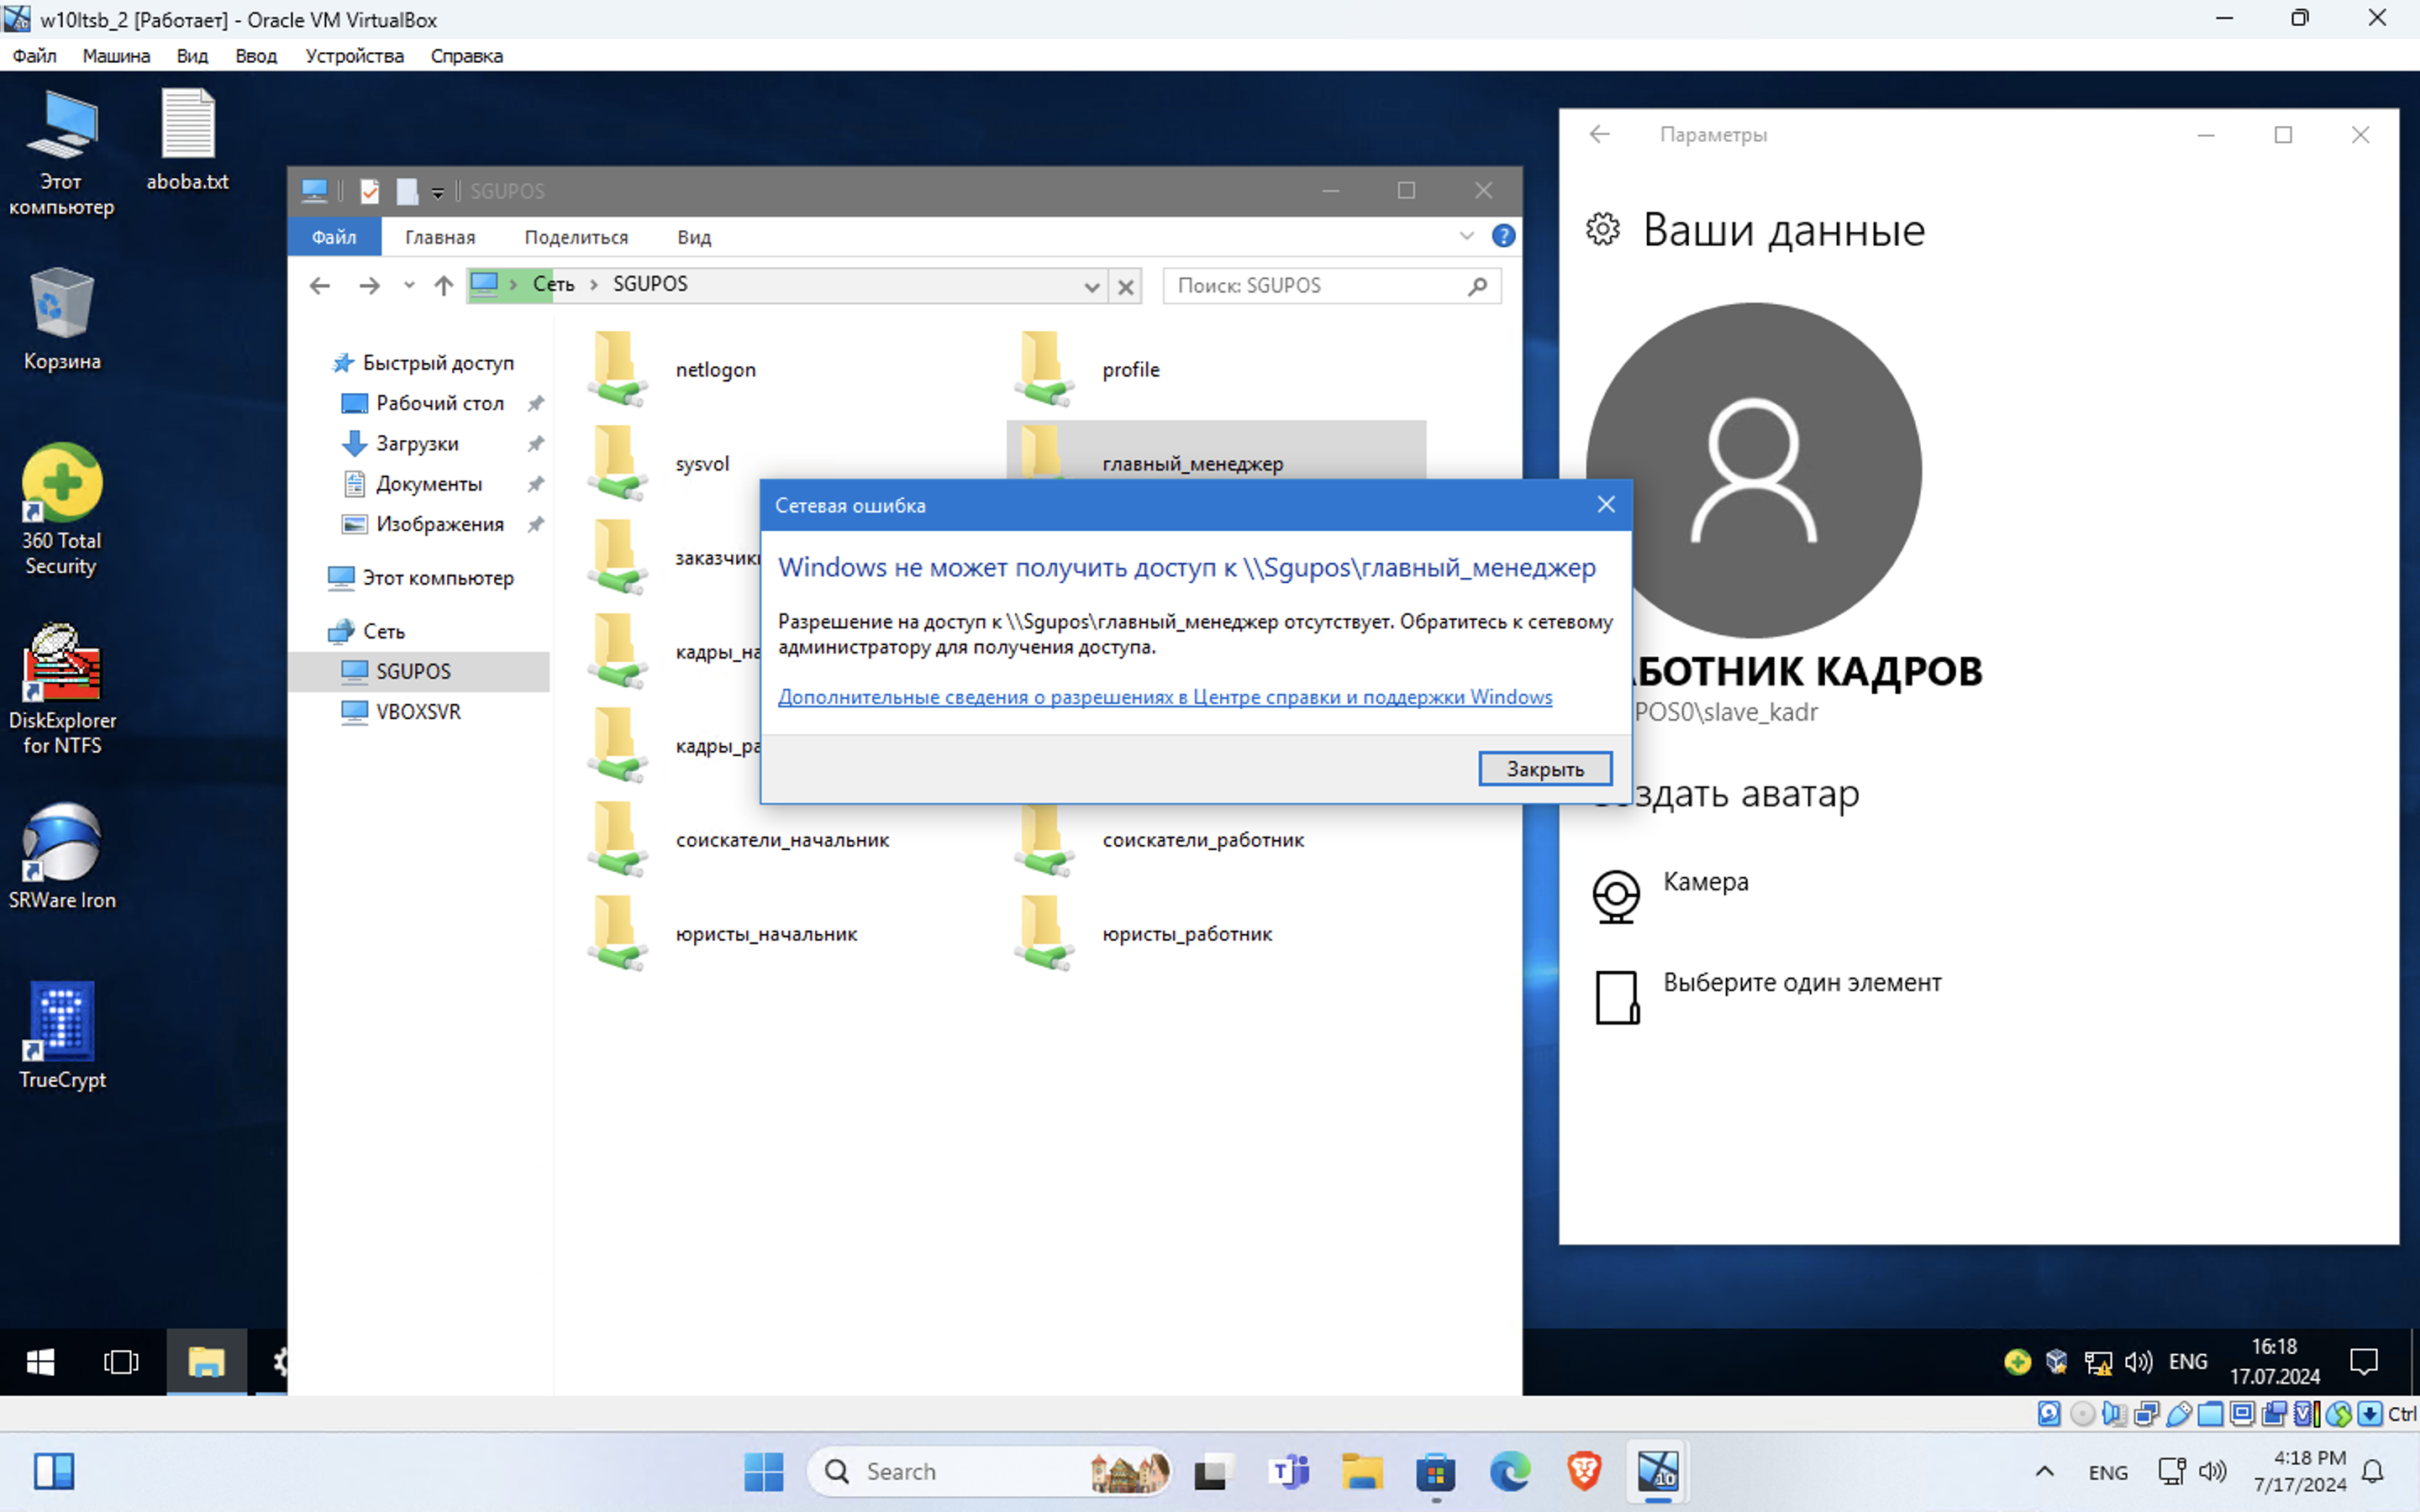
\includegraphics[width=1\textwidth]{pict/prac/31}
  \caption{Работник кадров -> Главный менеджер}
  \label{fig:30}
\end{figure}

\begin{figure}[H]
  \centering
  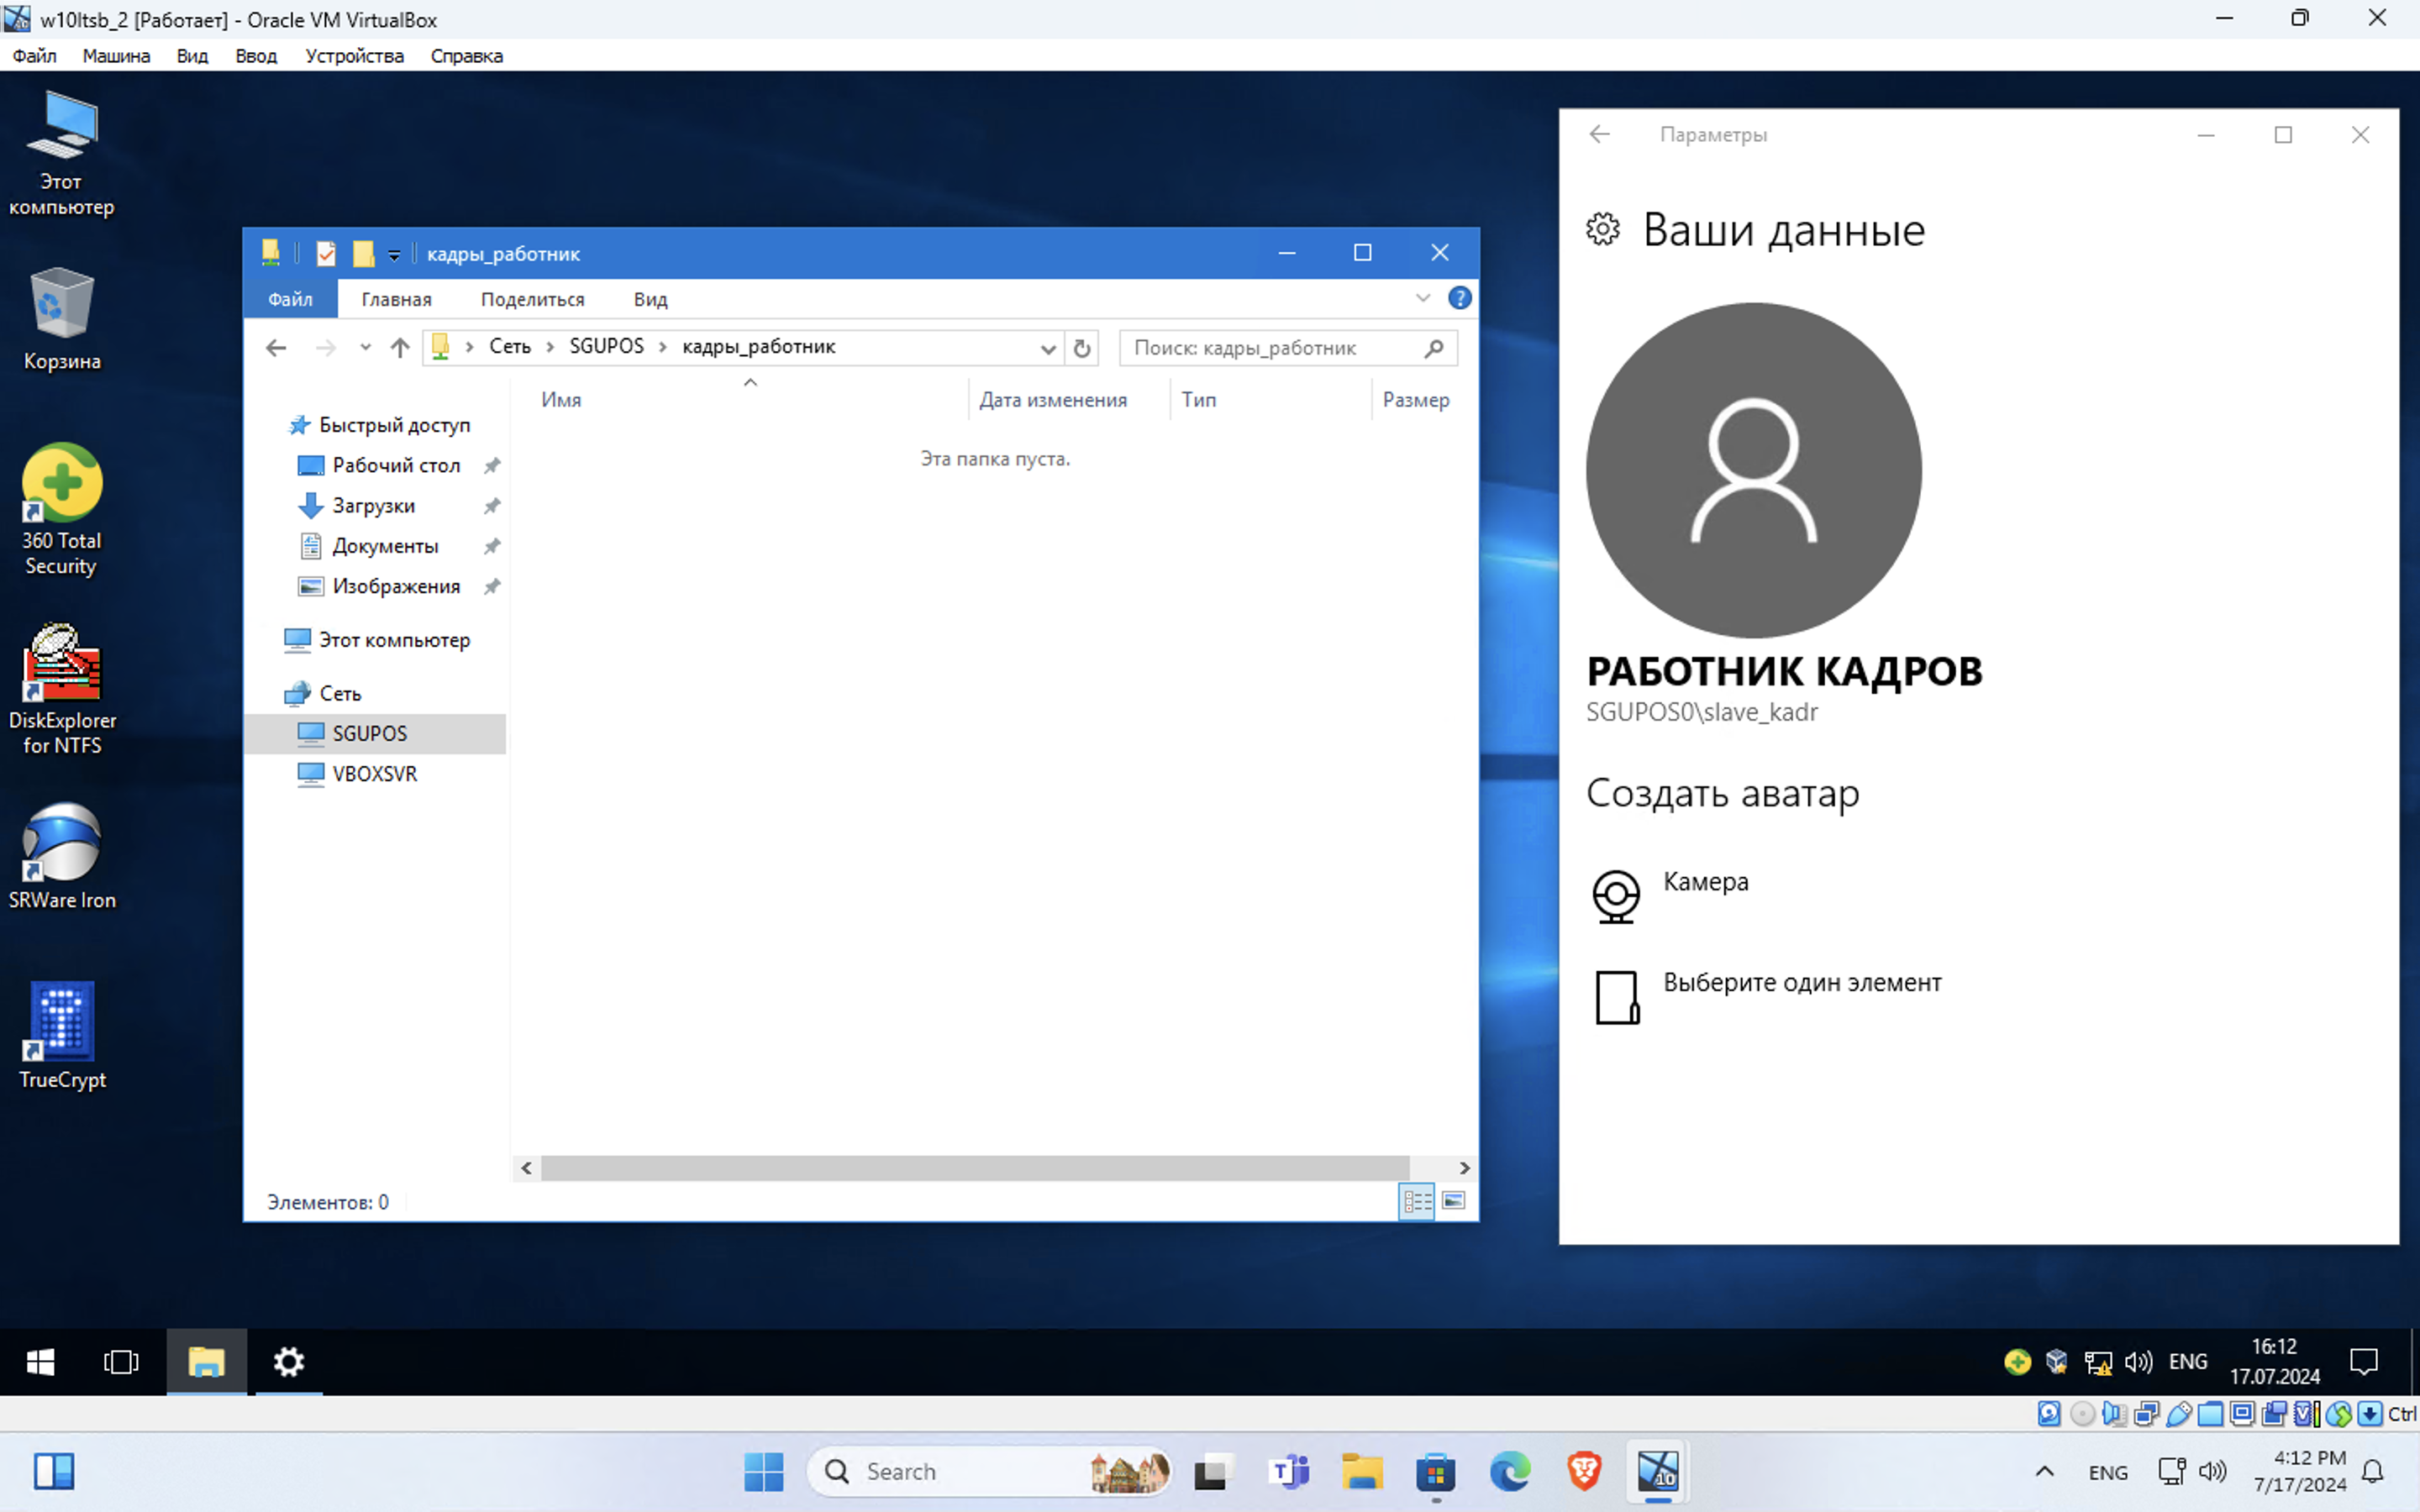
\includegraphics[width=1\textwidth]{pict/prac/28}
  \caption{Работник кадров -> Работник кадров}
  \label{fig:27}
\end{figure}


\begin{figure}[H]
  \centering
  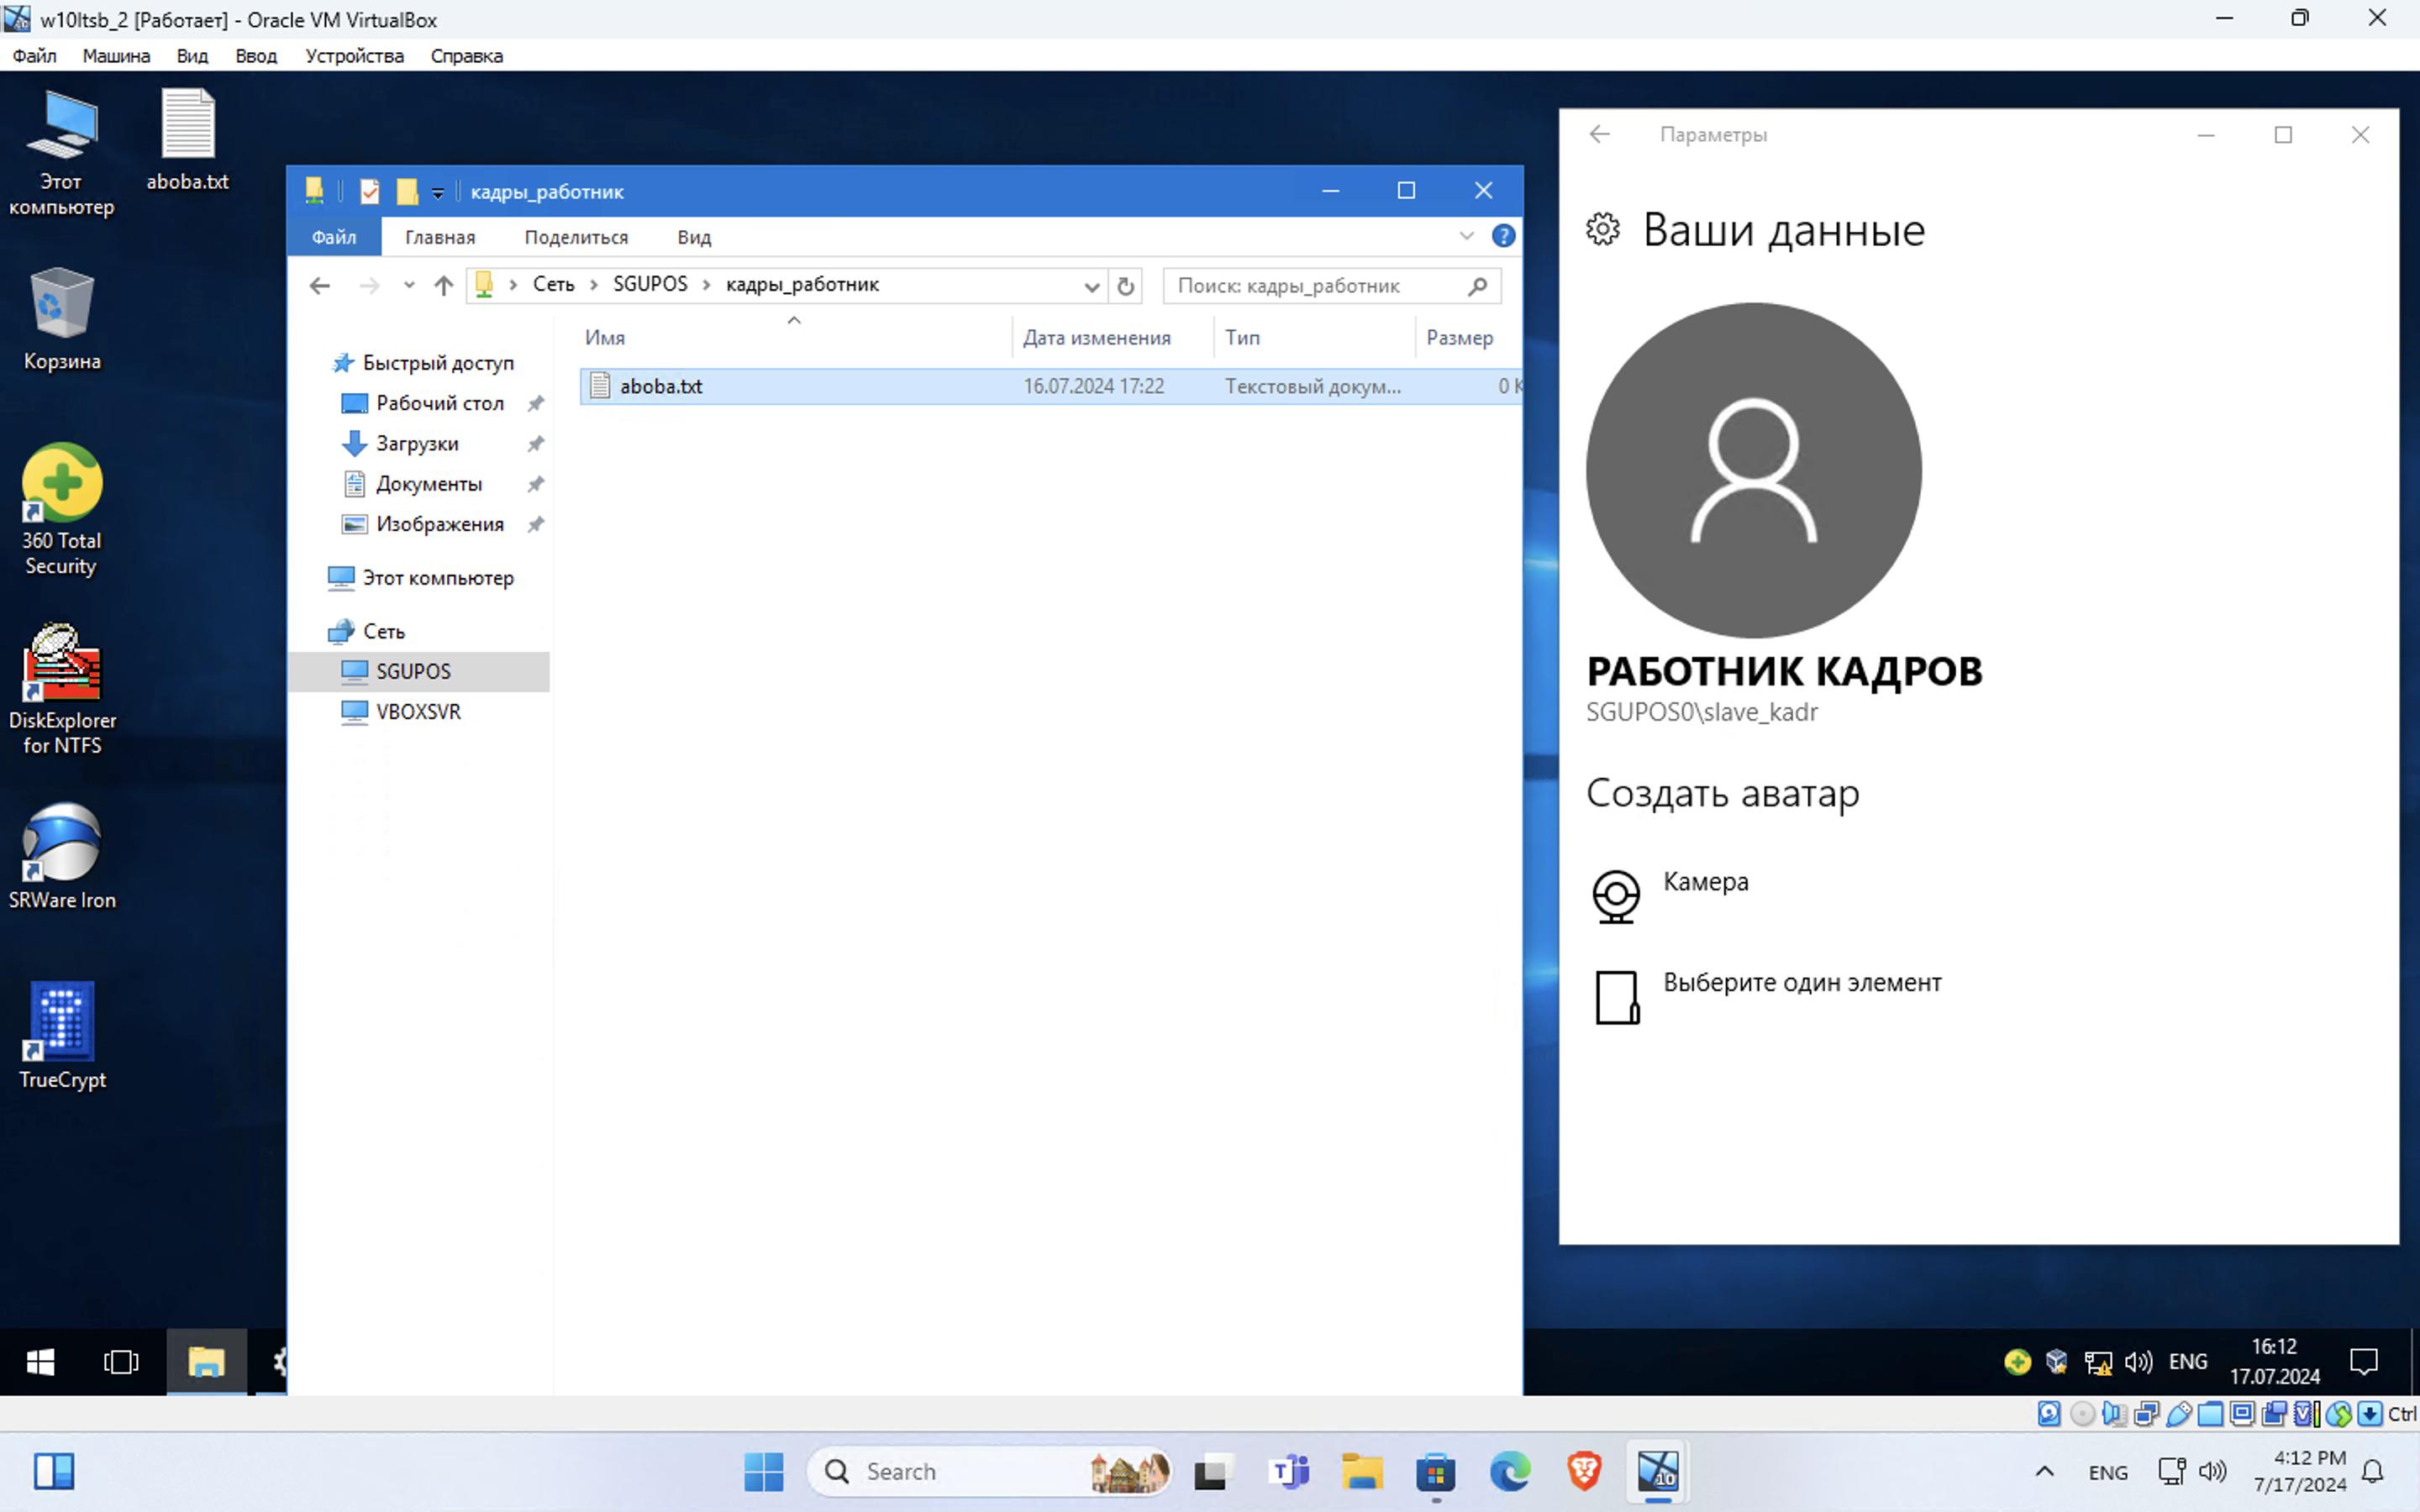
\includegraphics[width=1\textwidth]{pict/prac/29}
  \caption{Может создавать документы}
  \label{fig:28}
\end{figure}

\begin{figure}[H]
  \centering
  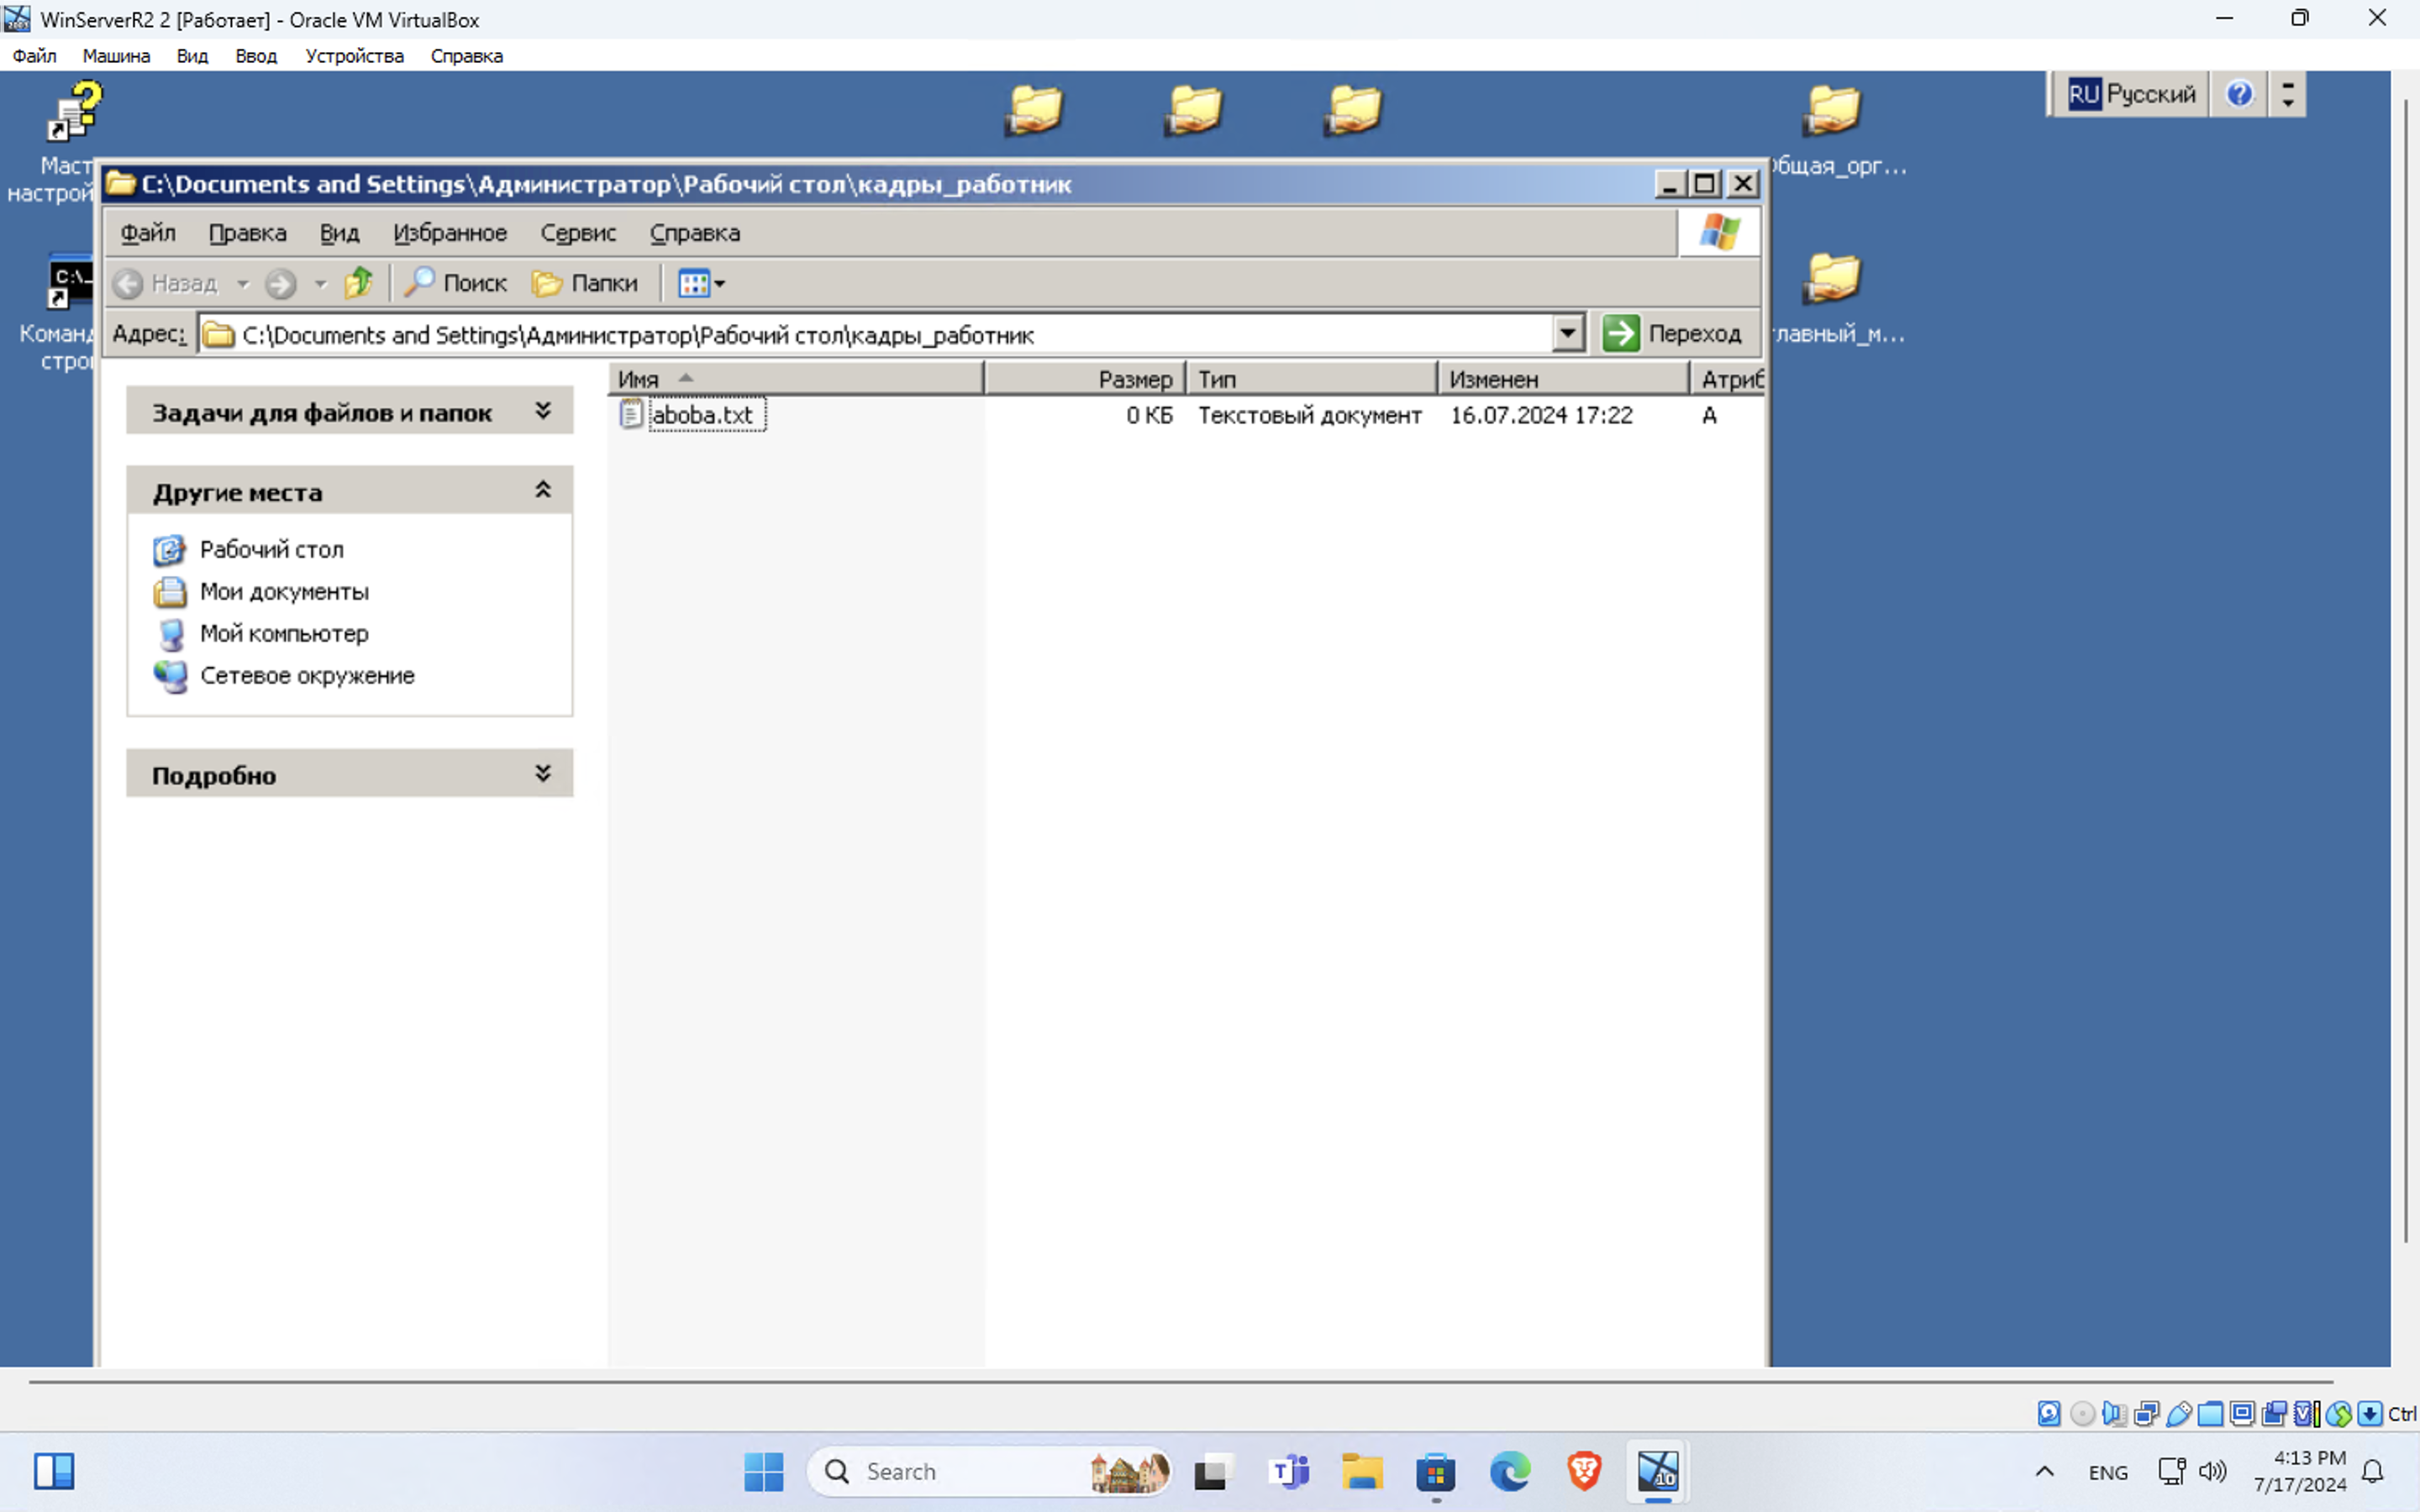
\includegraphics[width=1\textwidth]{pict/prac/30}
  \caption{Созданный работником документ на сервере}
  \label{fig:29}
\end{figure}


\begin{figure}[H]
  \centering
  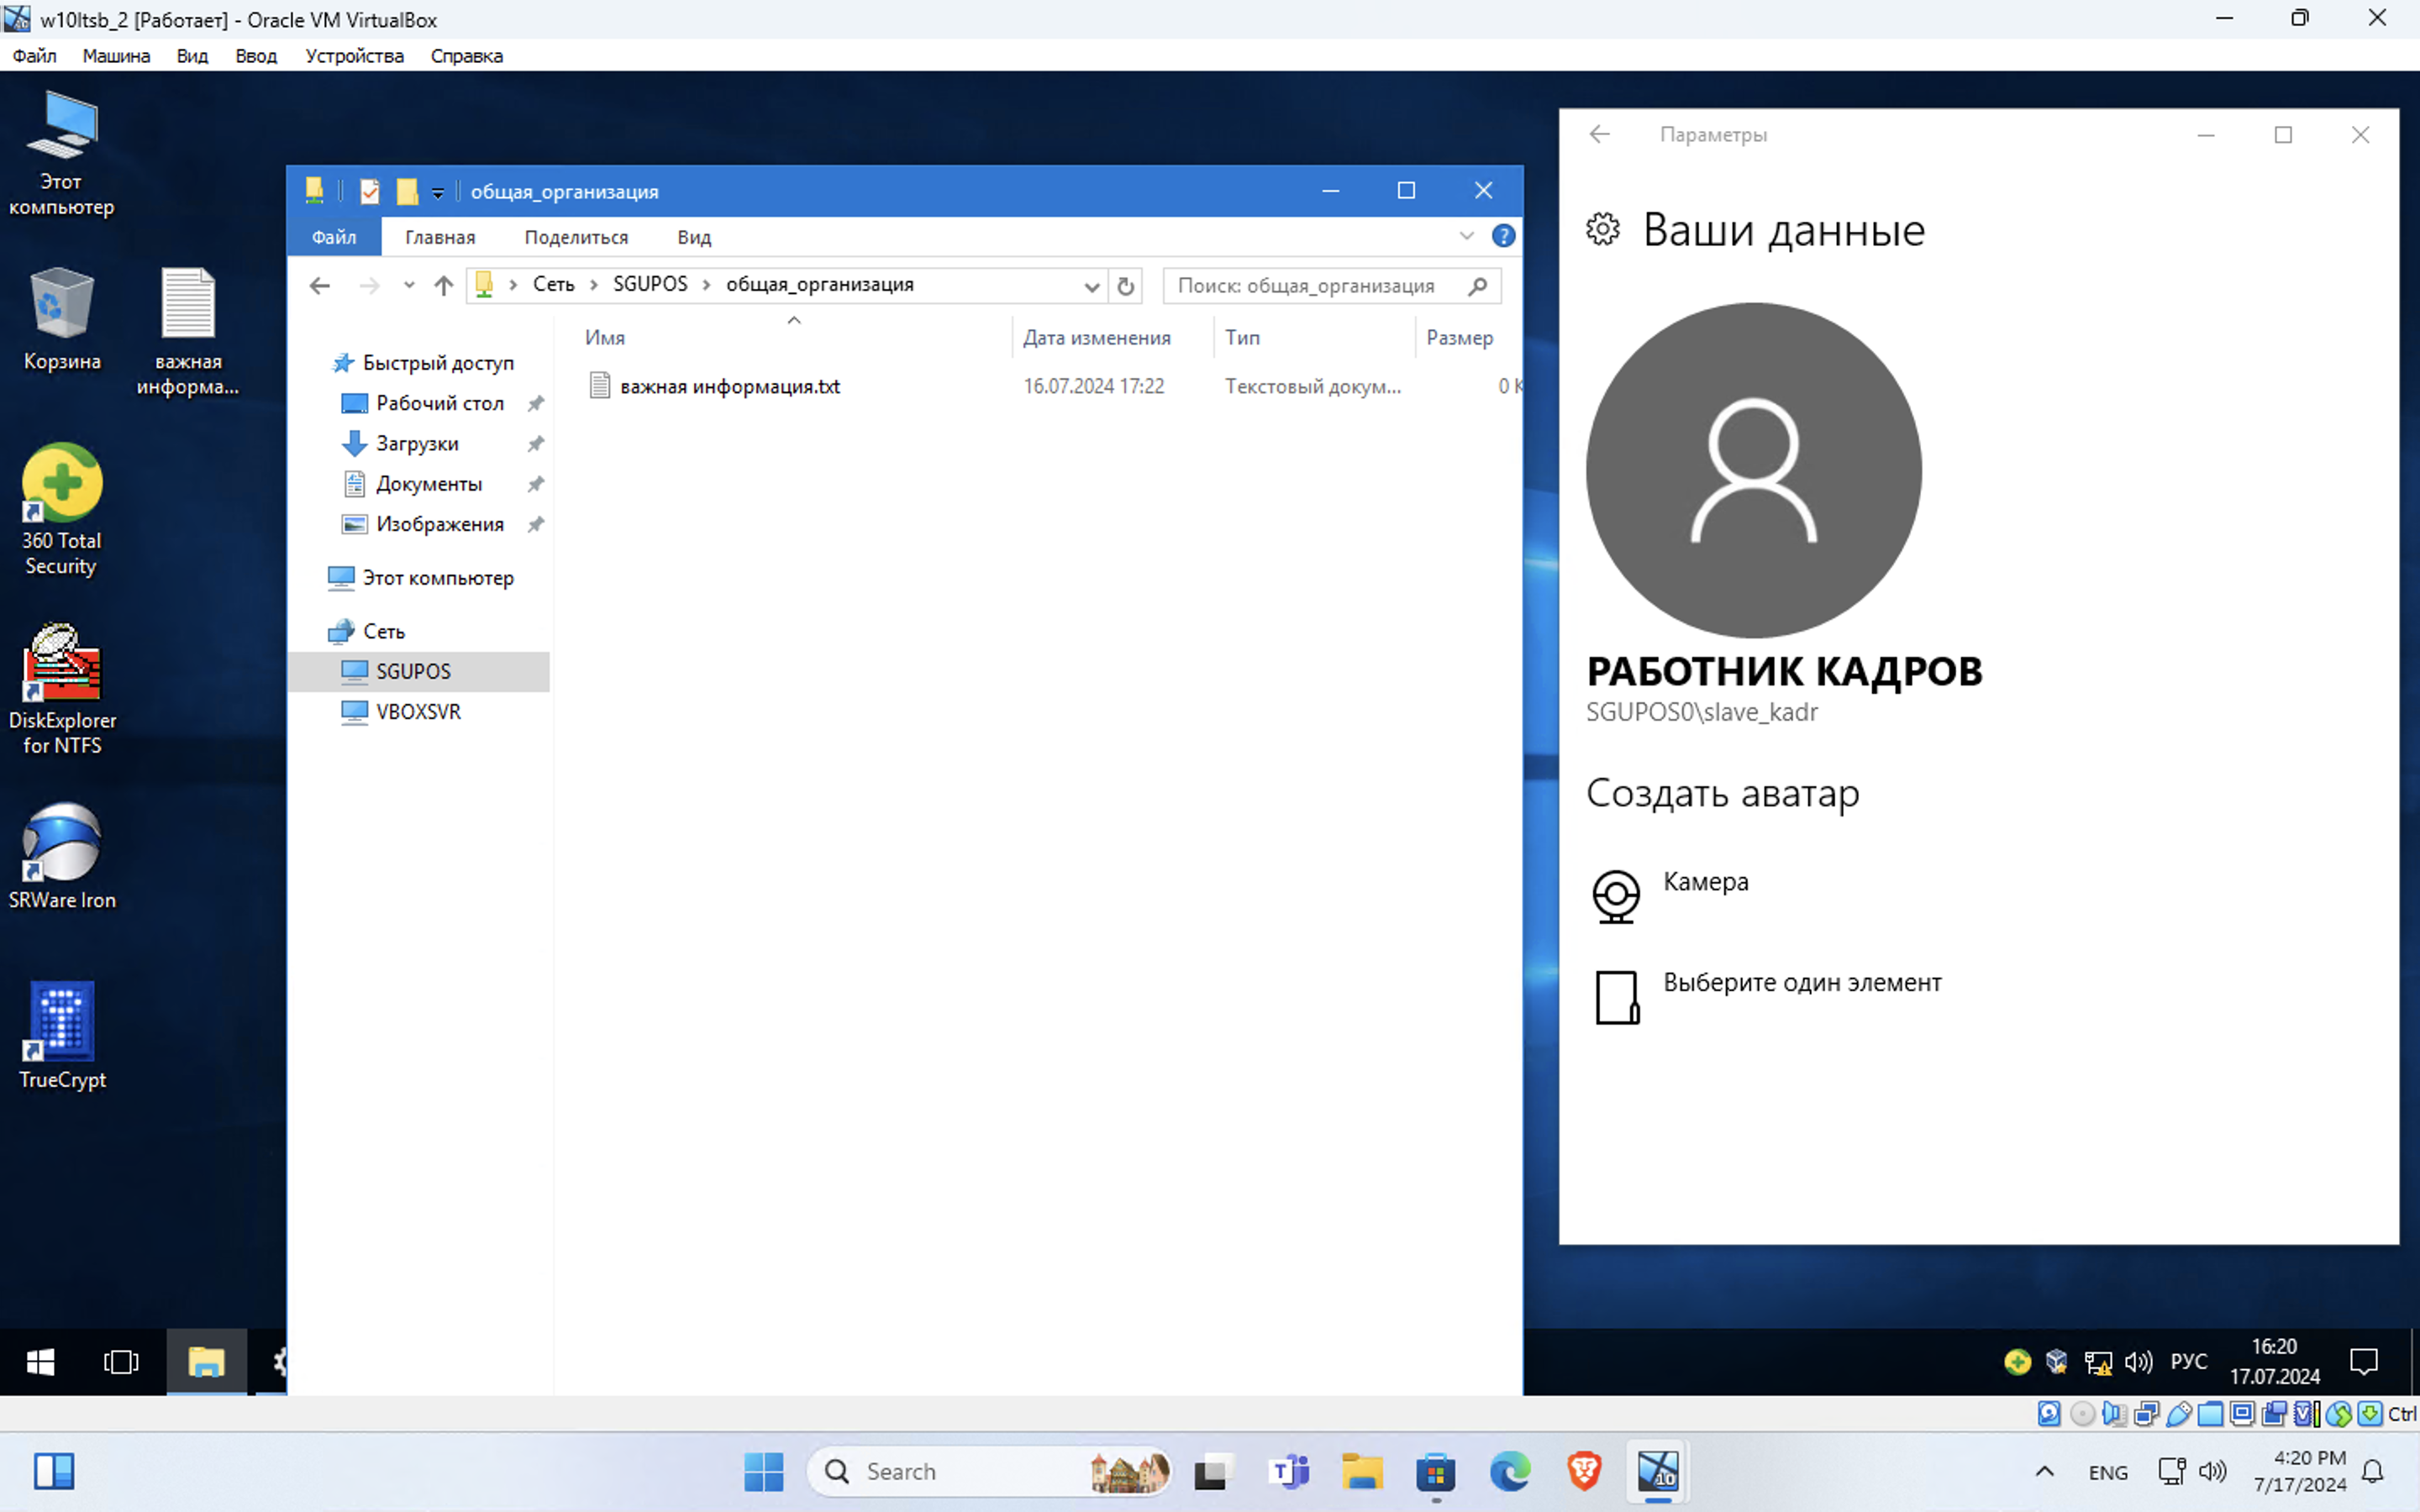
\includegraphics[width=1\textwidth]{pict/prac/33}
  \caption{Создание документа в общей папке}
  \label{fig:32}
\end{figure}

\begin{figure}[H]
  \centering
  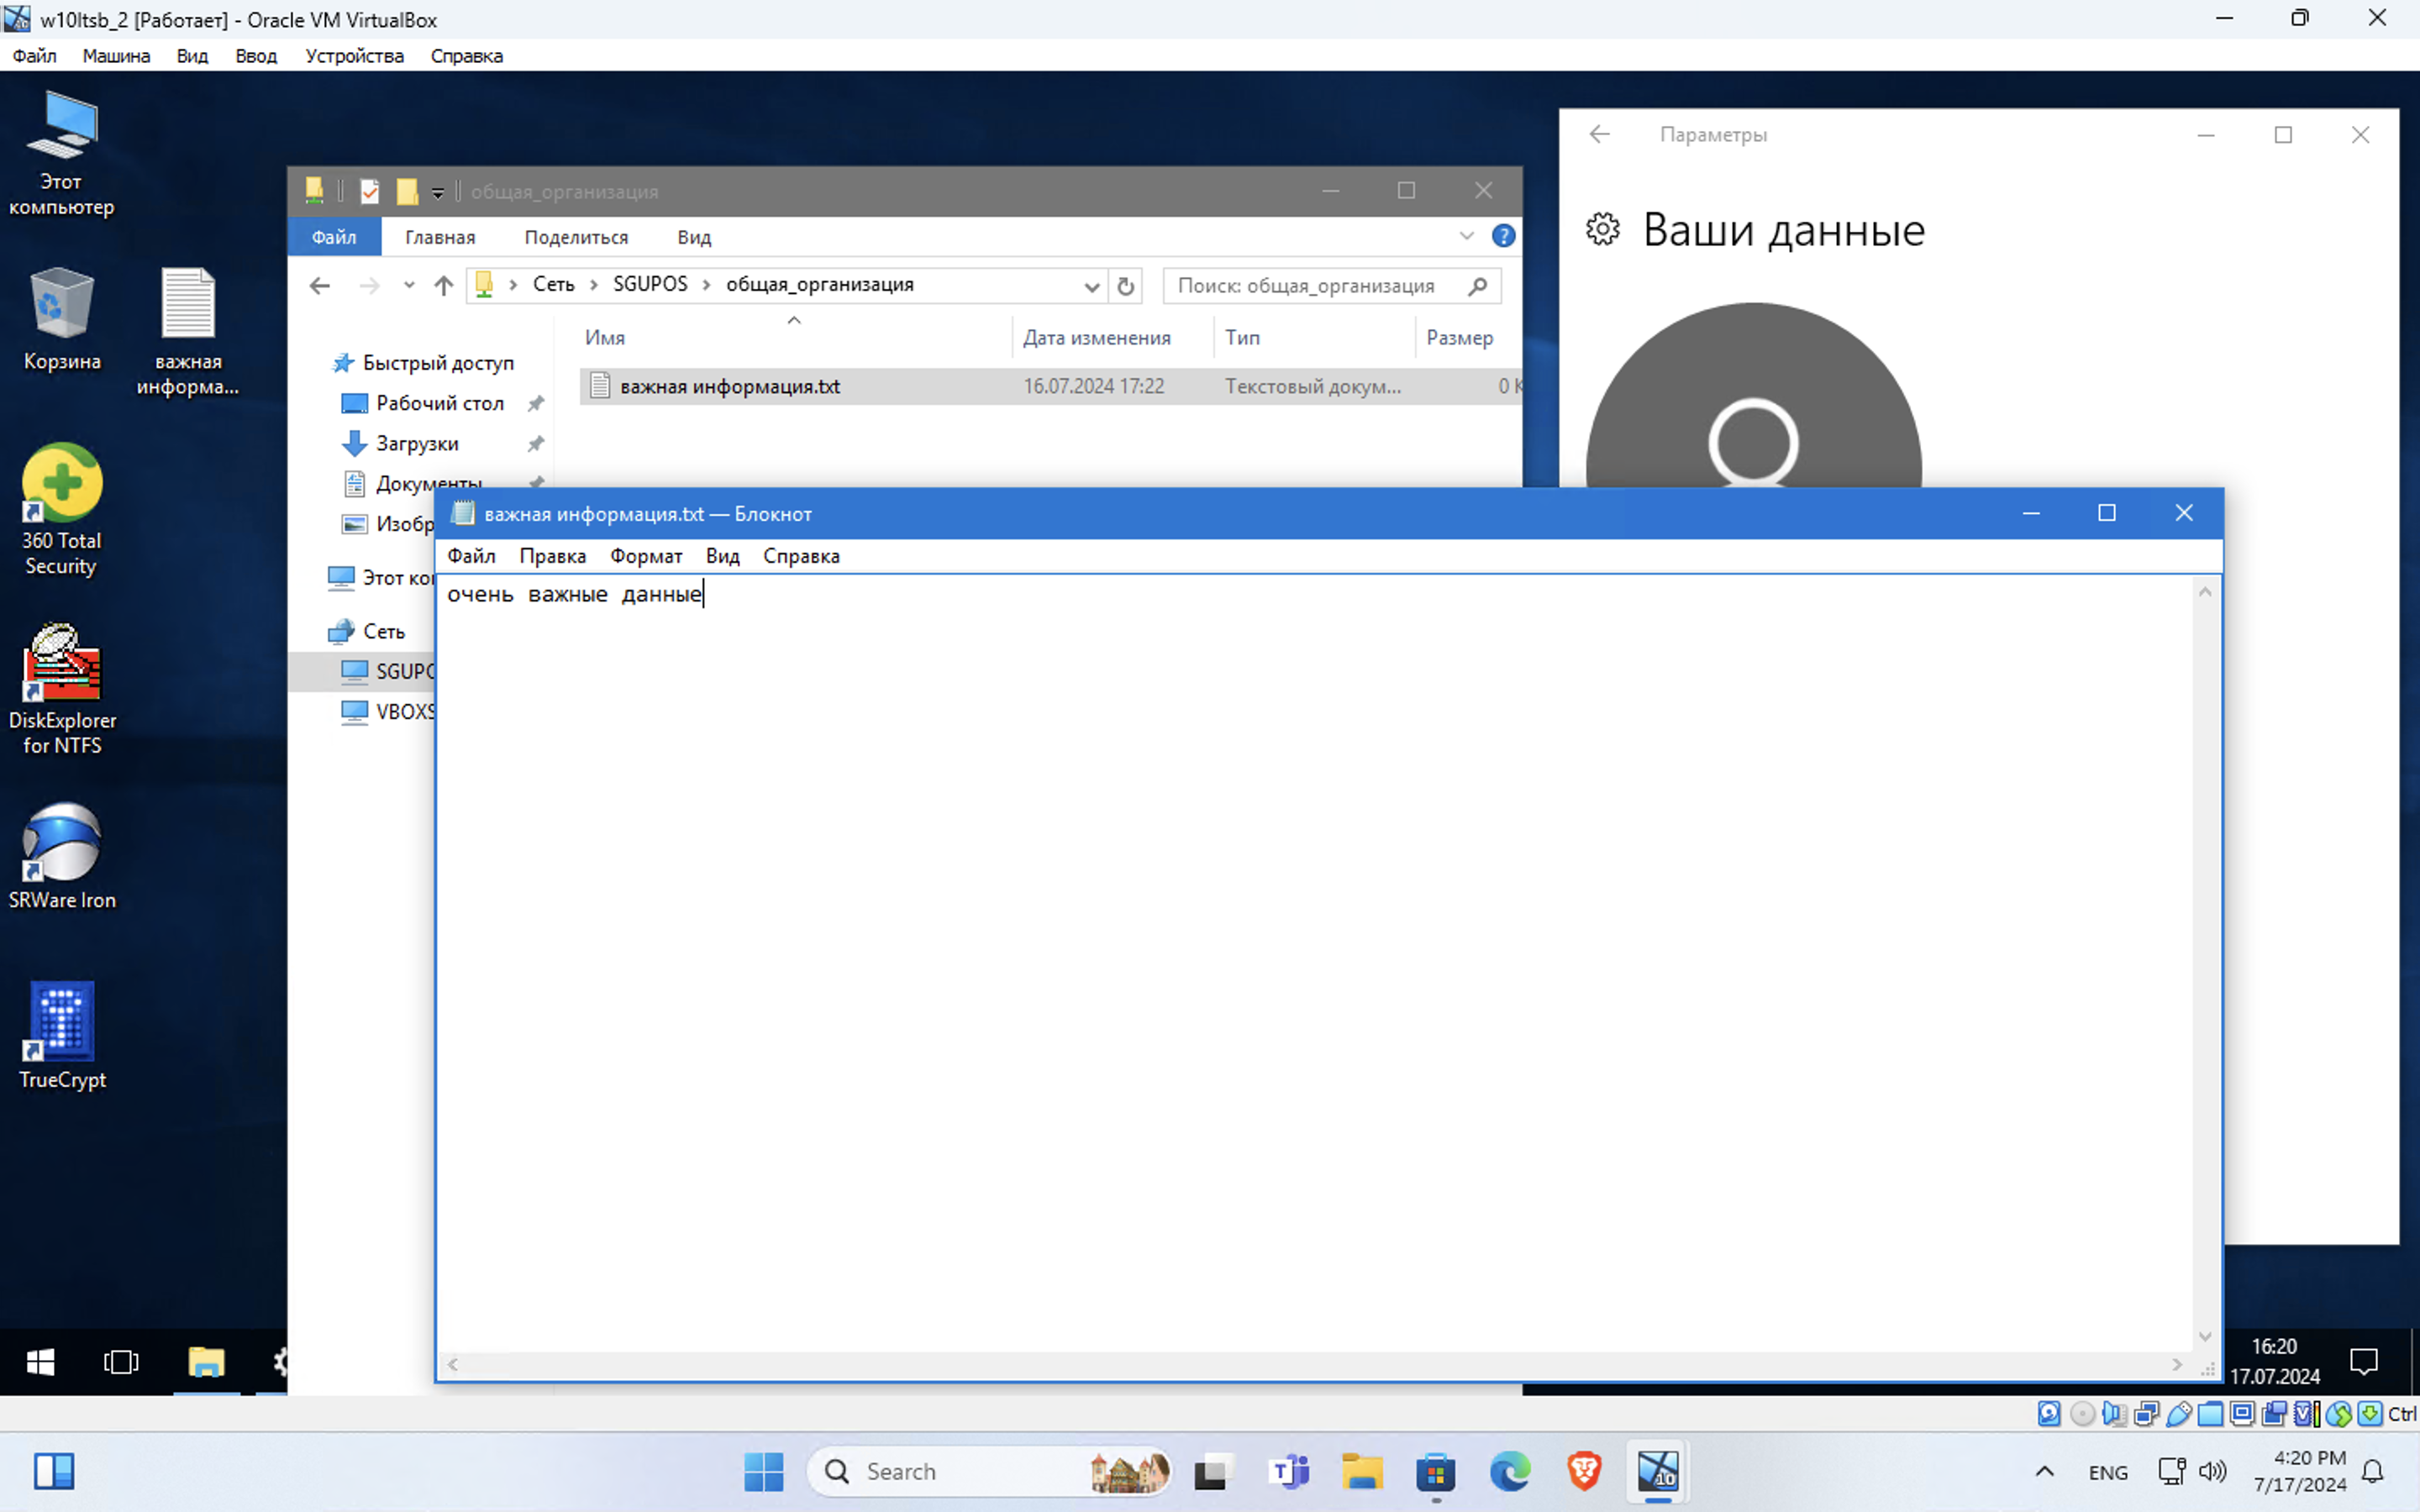
\includegraphics[width=1\textwidth]{pict/prac/34}
  \caption{Создание документа в общей папке}
  \label{fig:33}
\end{figure}

Рассмотрим аккаунт начальника подразделения соискателей и его доступ.
\begin{figure}[H]
  \centering
  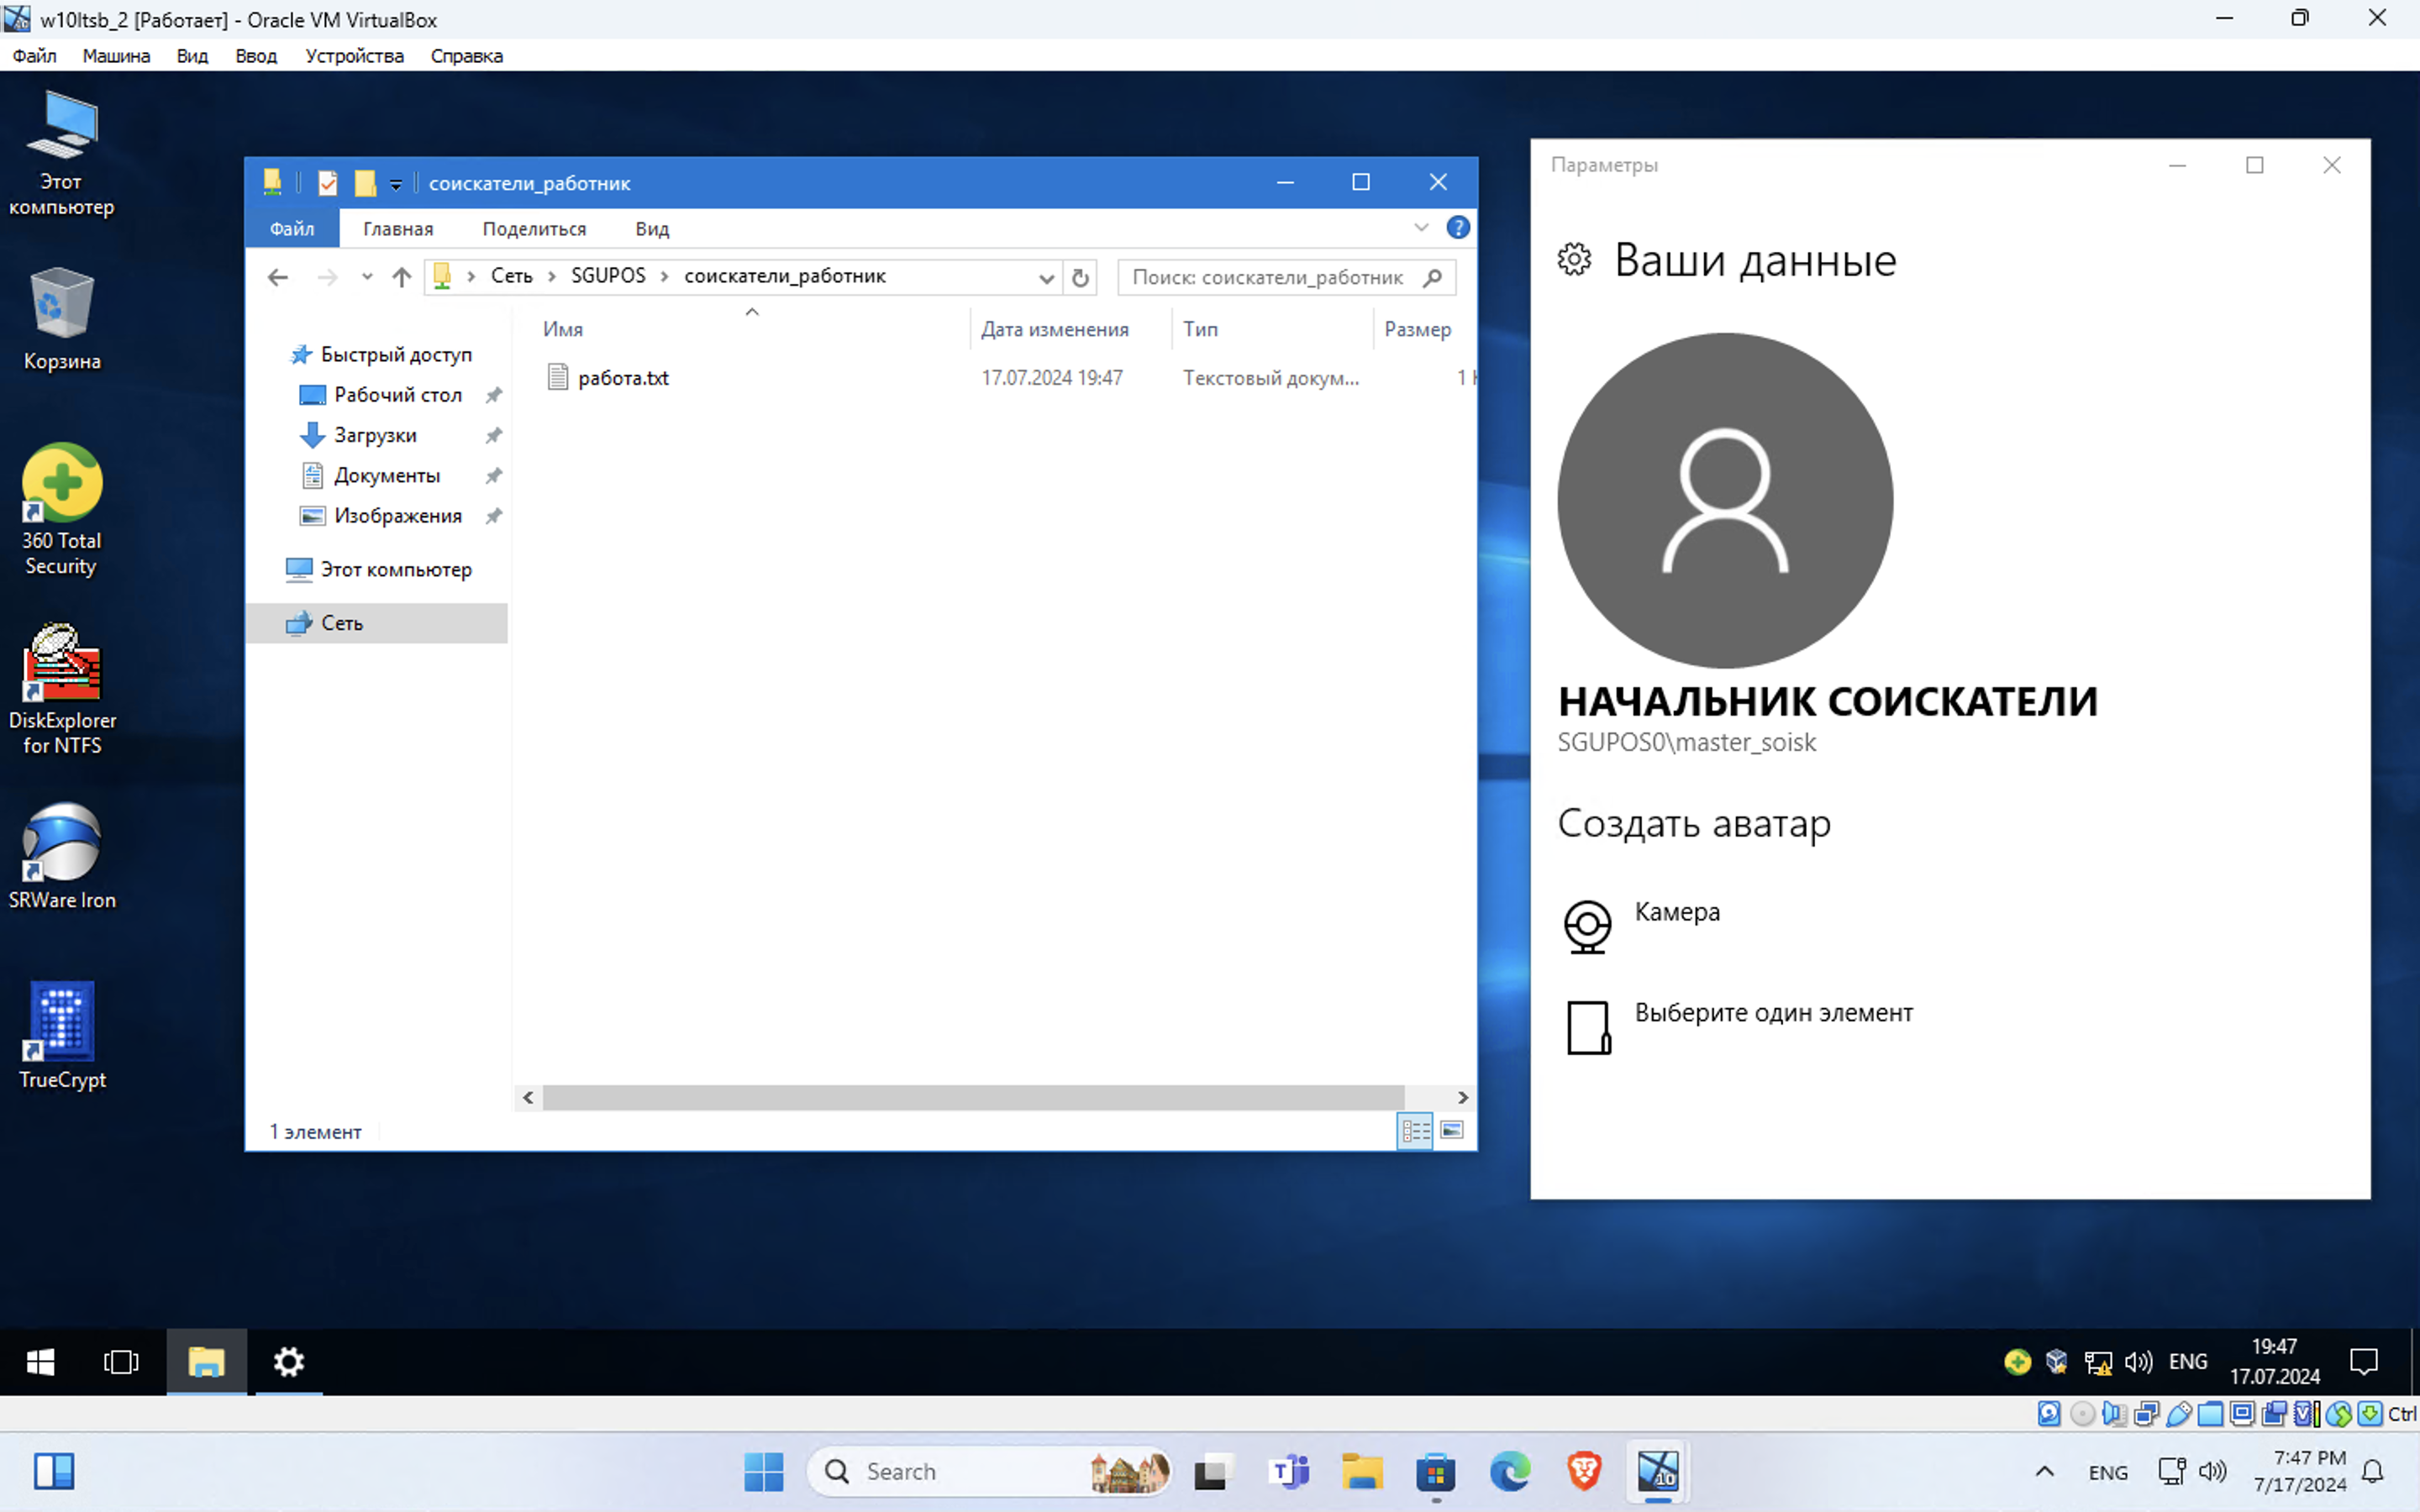
\includegraphics[width=1\textwidth]{pict/prac/35}
  \caption{Начальник соискателей -> Работник соискателей}
  \label{fig:34}
\end{figure}

\begin{figure}[H]
  \centering
  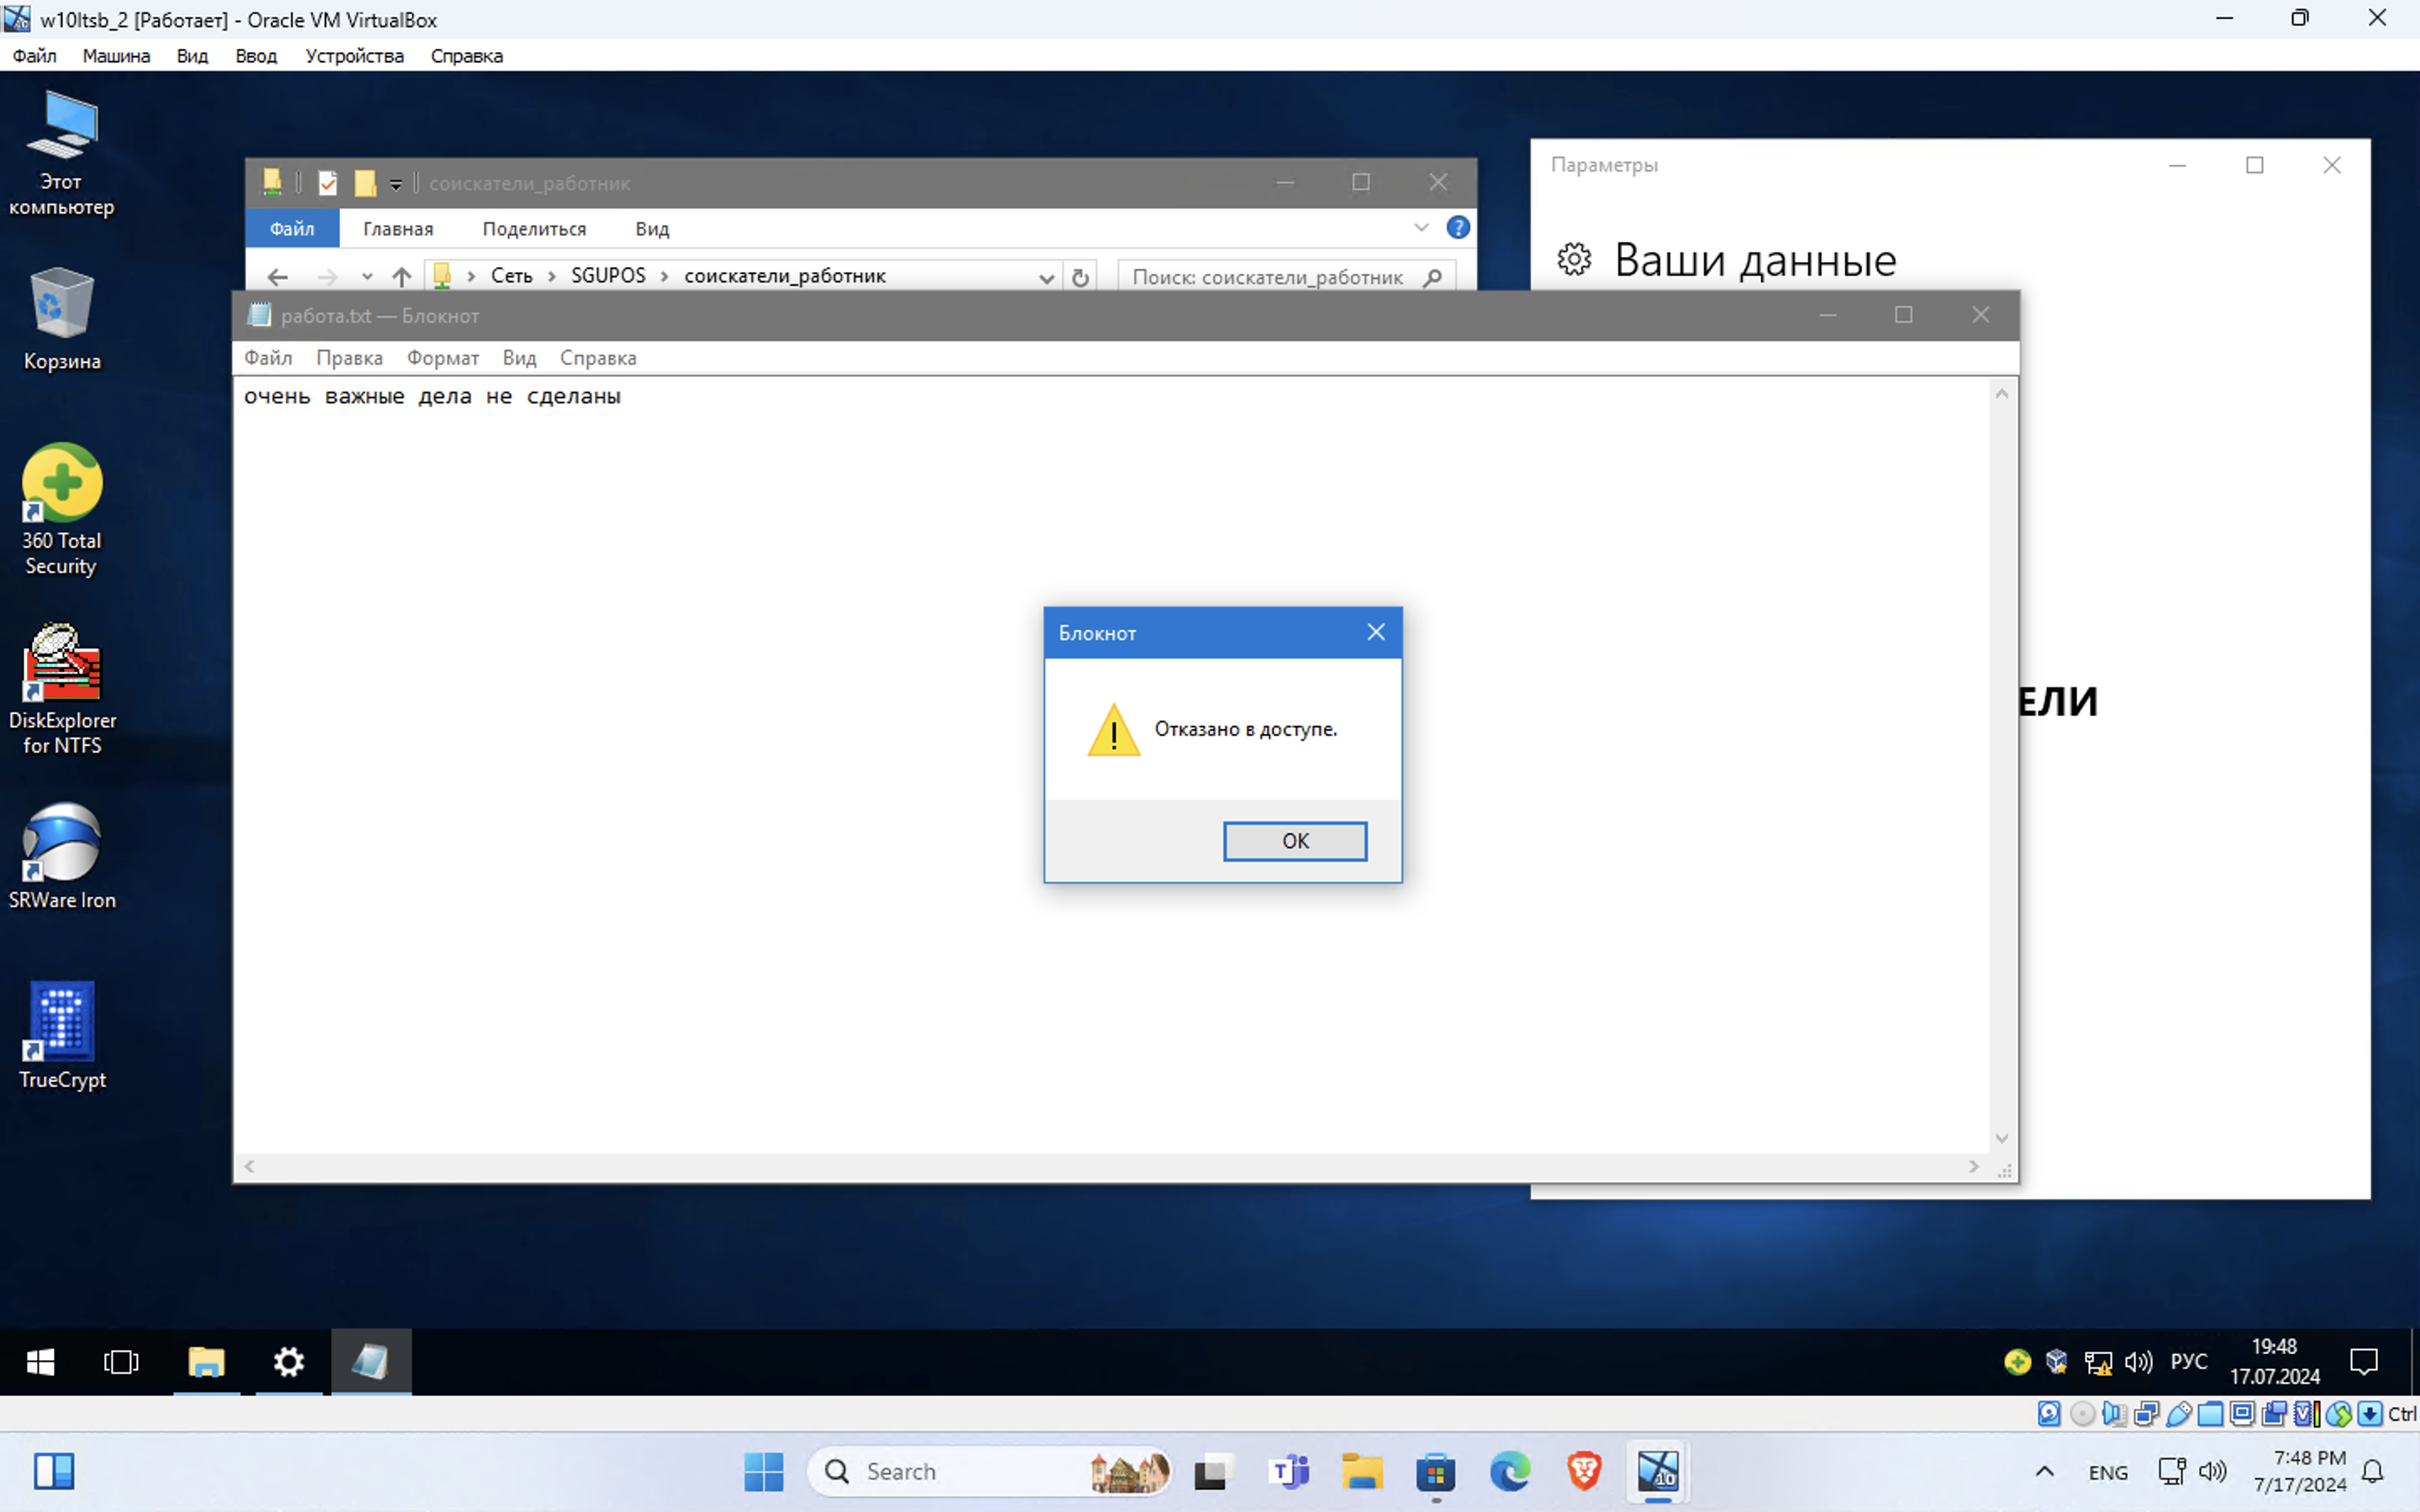
\includegraphics[width=1\textwidth]{pict/prac/36}
  \caption{Изменение документа в папке своего работника}
  \label{fig:35}
\end{figure}

\begin{figure}[H]
  \centering
  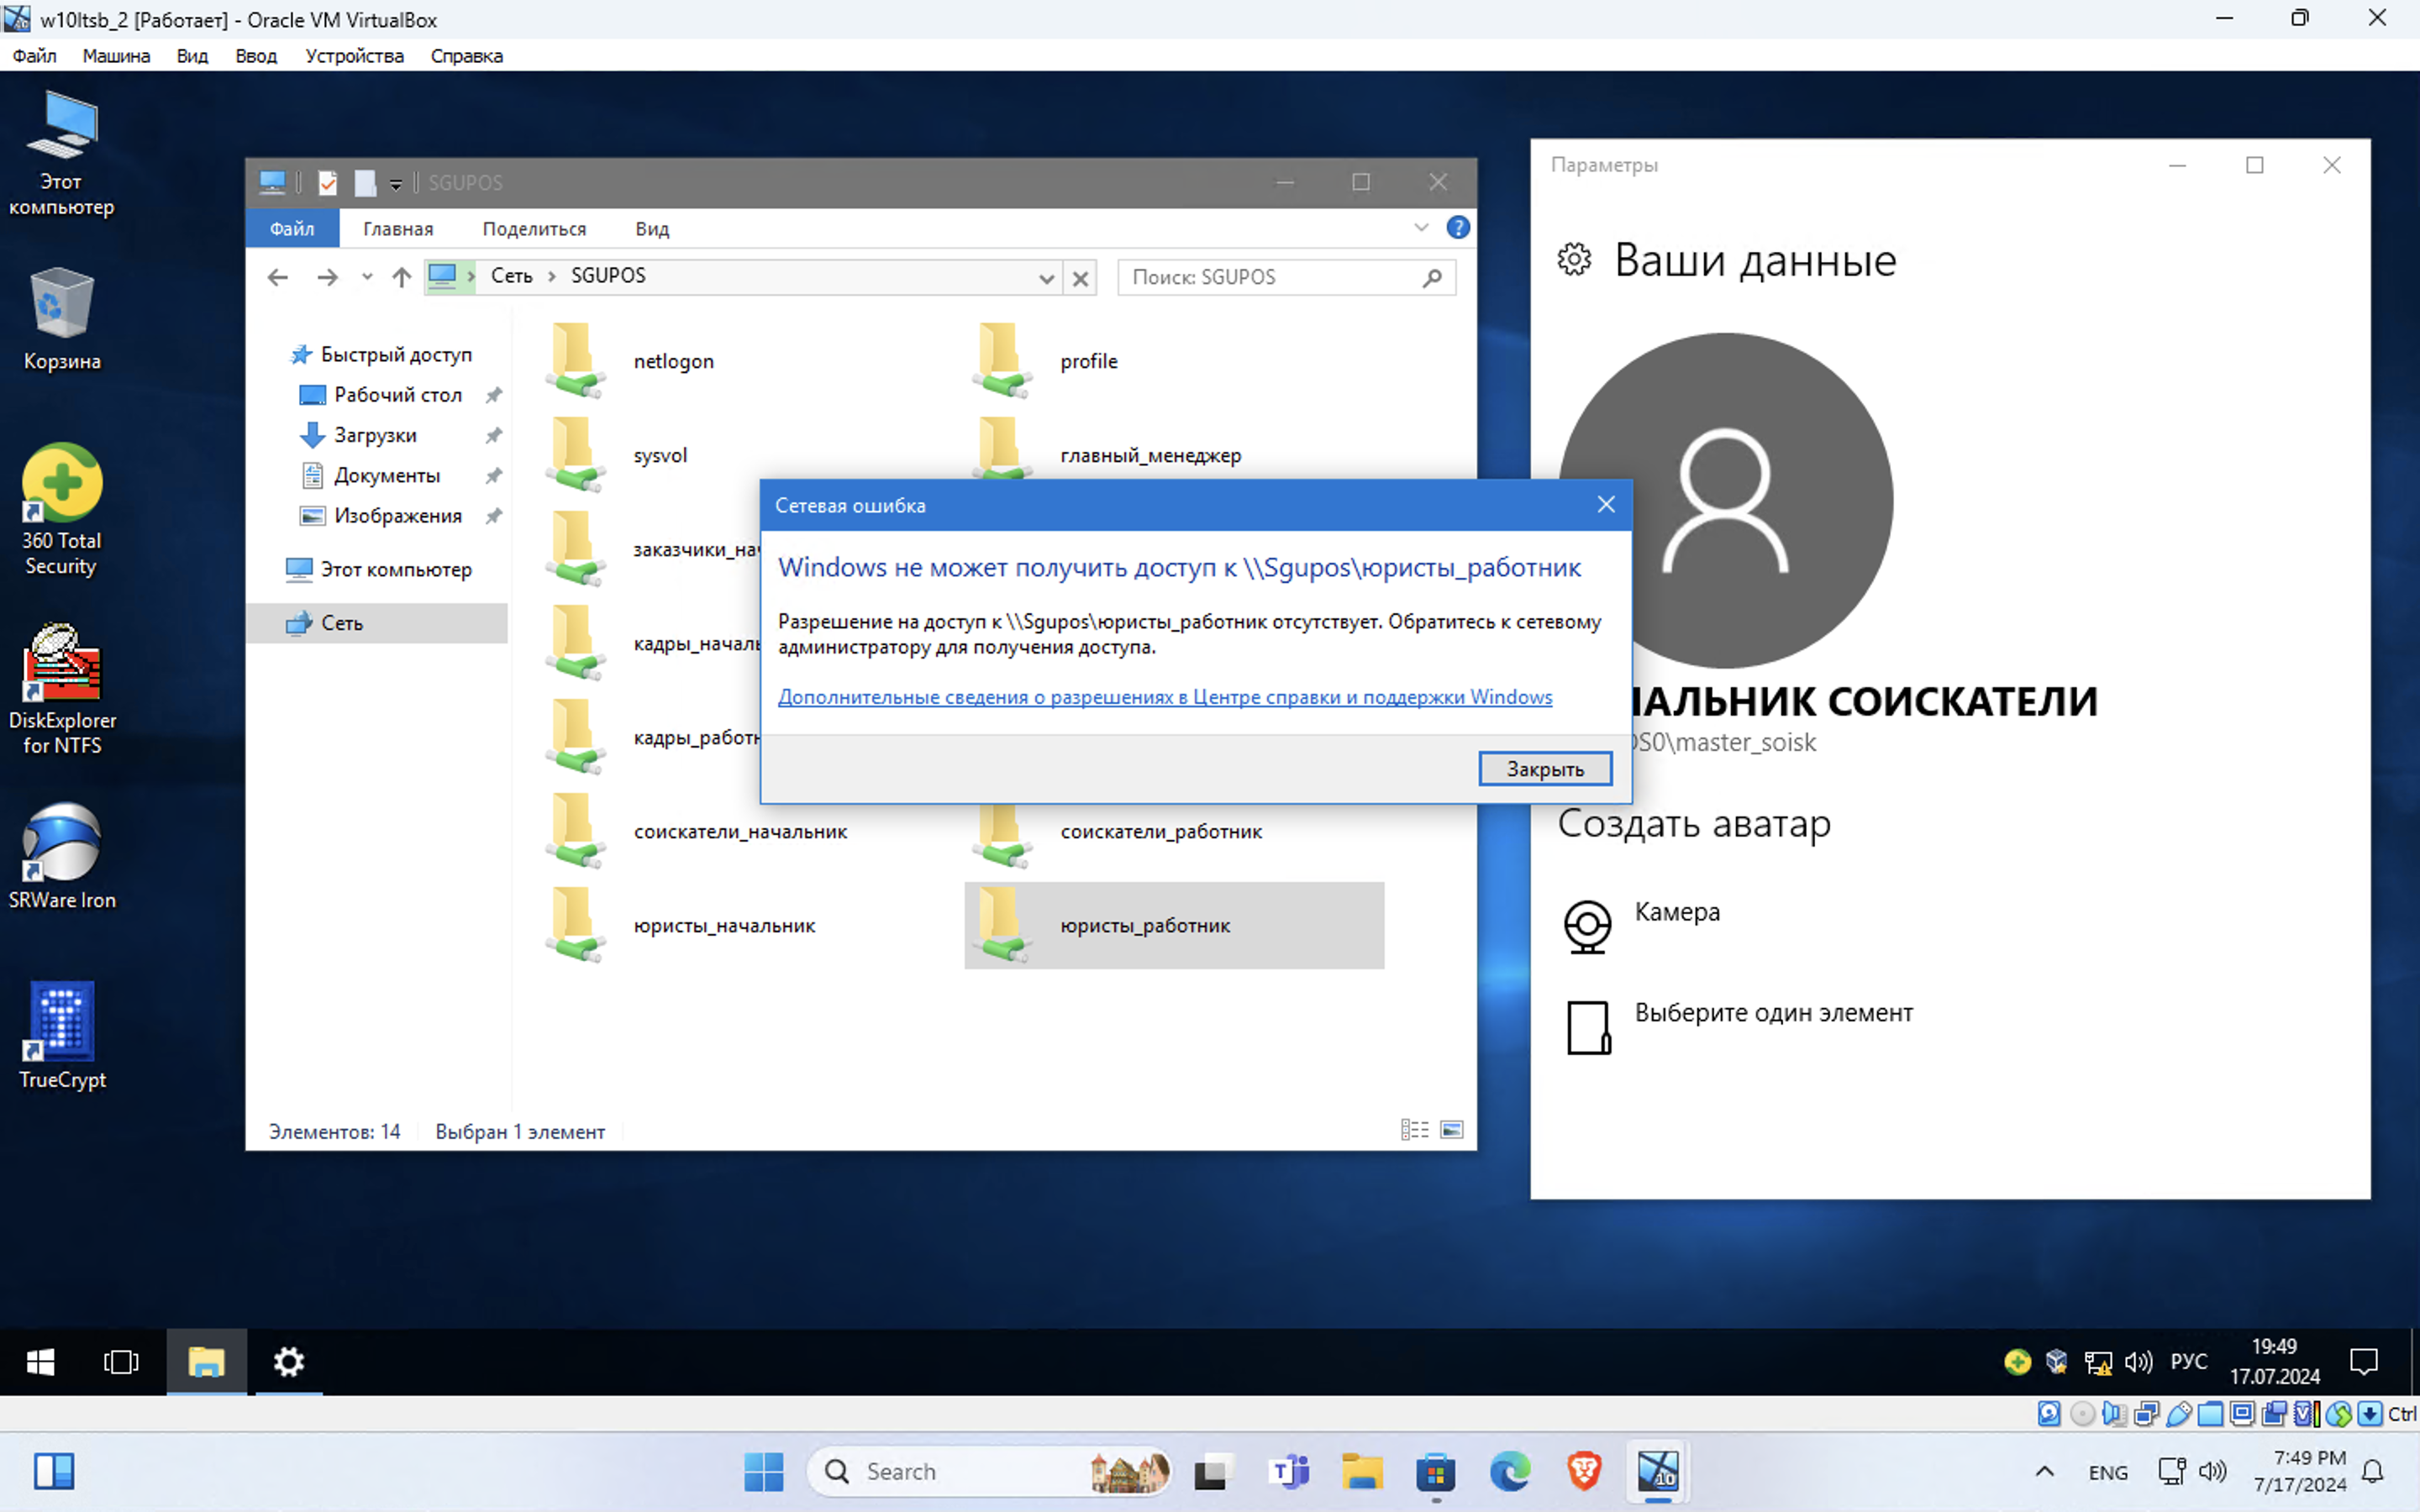
\includegraphics[width=1\textwidth]{pict/prac/39}
  \caption{Начальник соискателей -> Работник юрист}
  \label{fig:38}
\end{figure}

\begin{figure}[H]
  \centering
  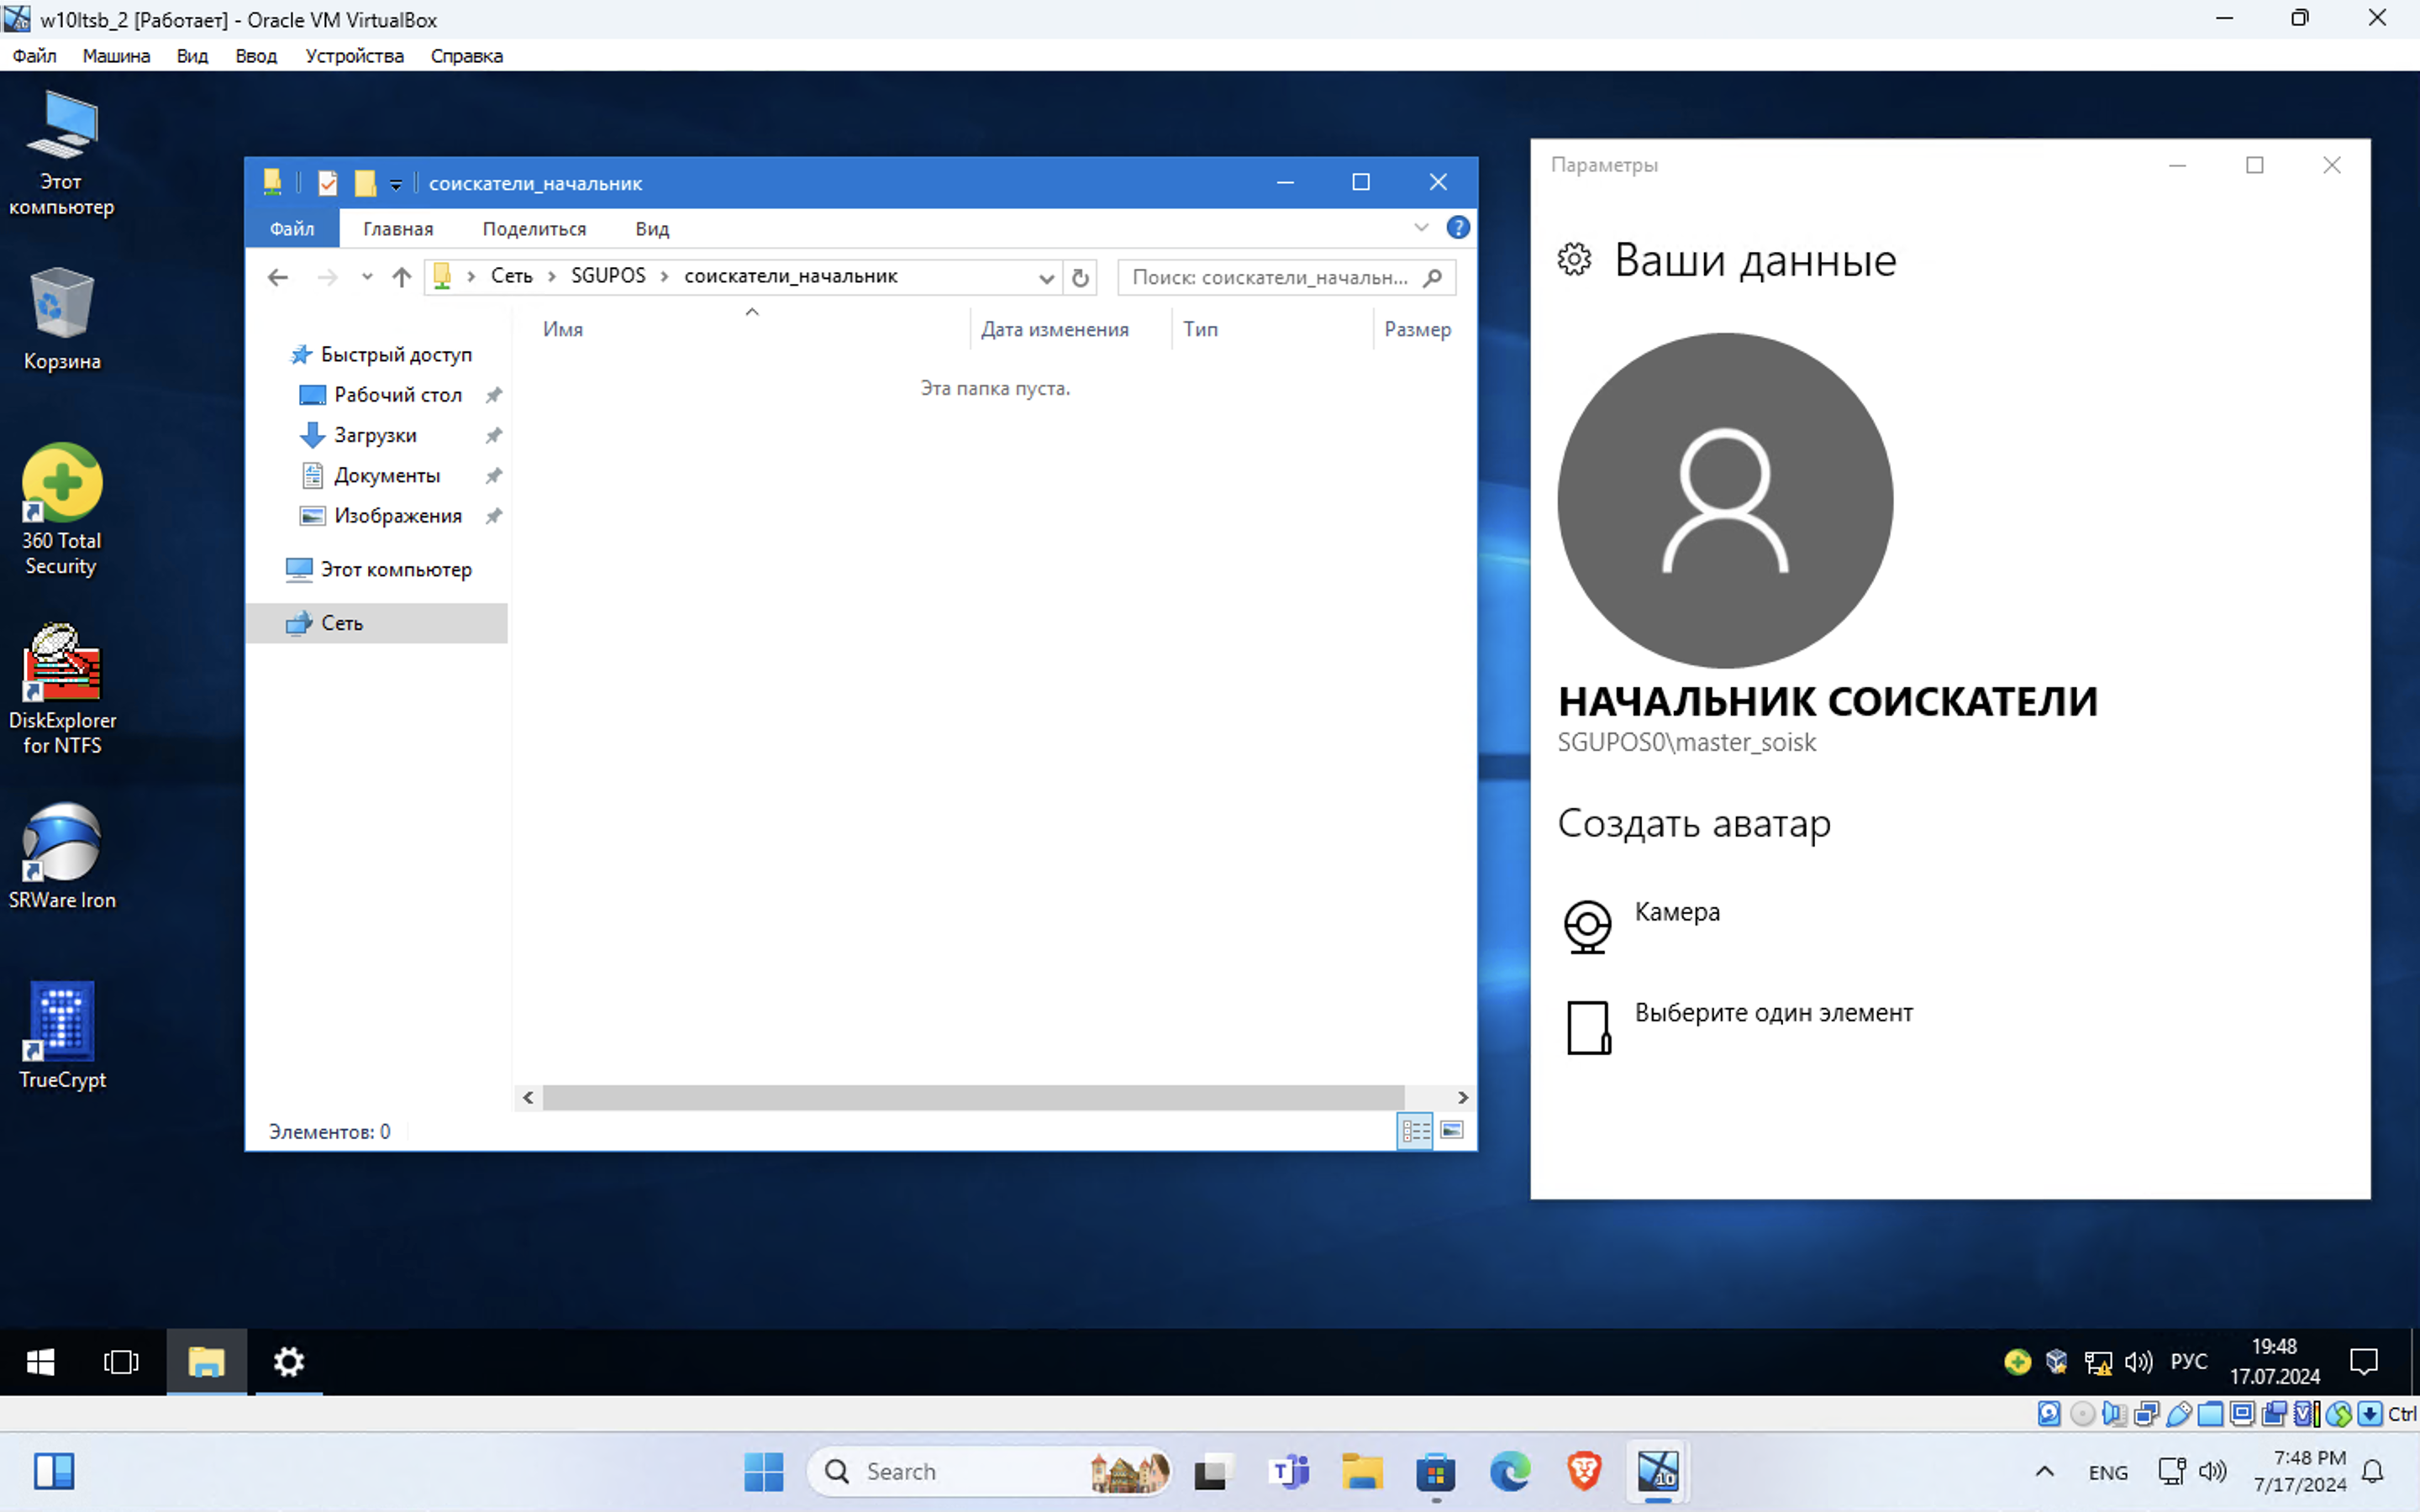
\includegraphics[width=1\textwidth]{pict/prac/37}
  \caption{Начальник соискателей -> Начальник соискателей}
  \label{fig:36}
\end{figure}

\begin{figure}[H]
  \centering
  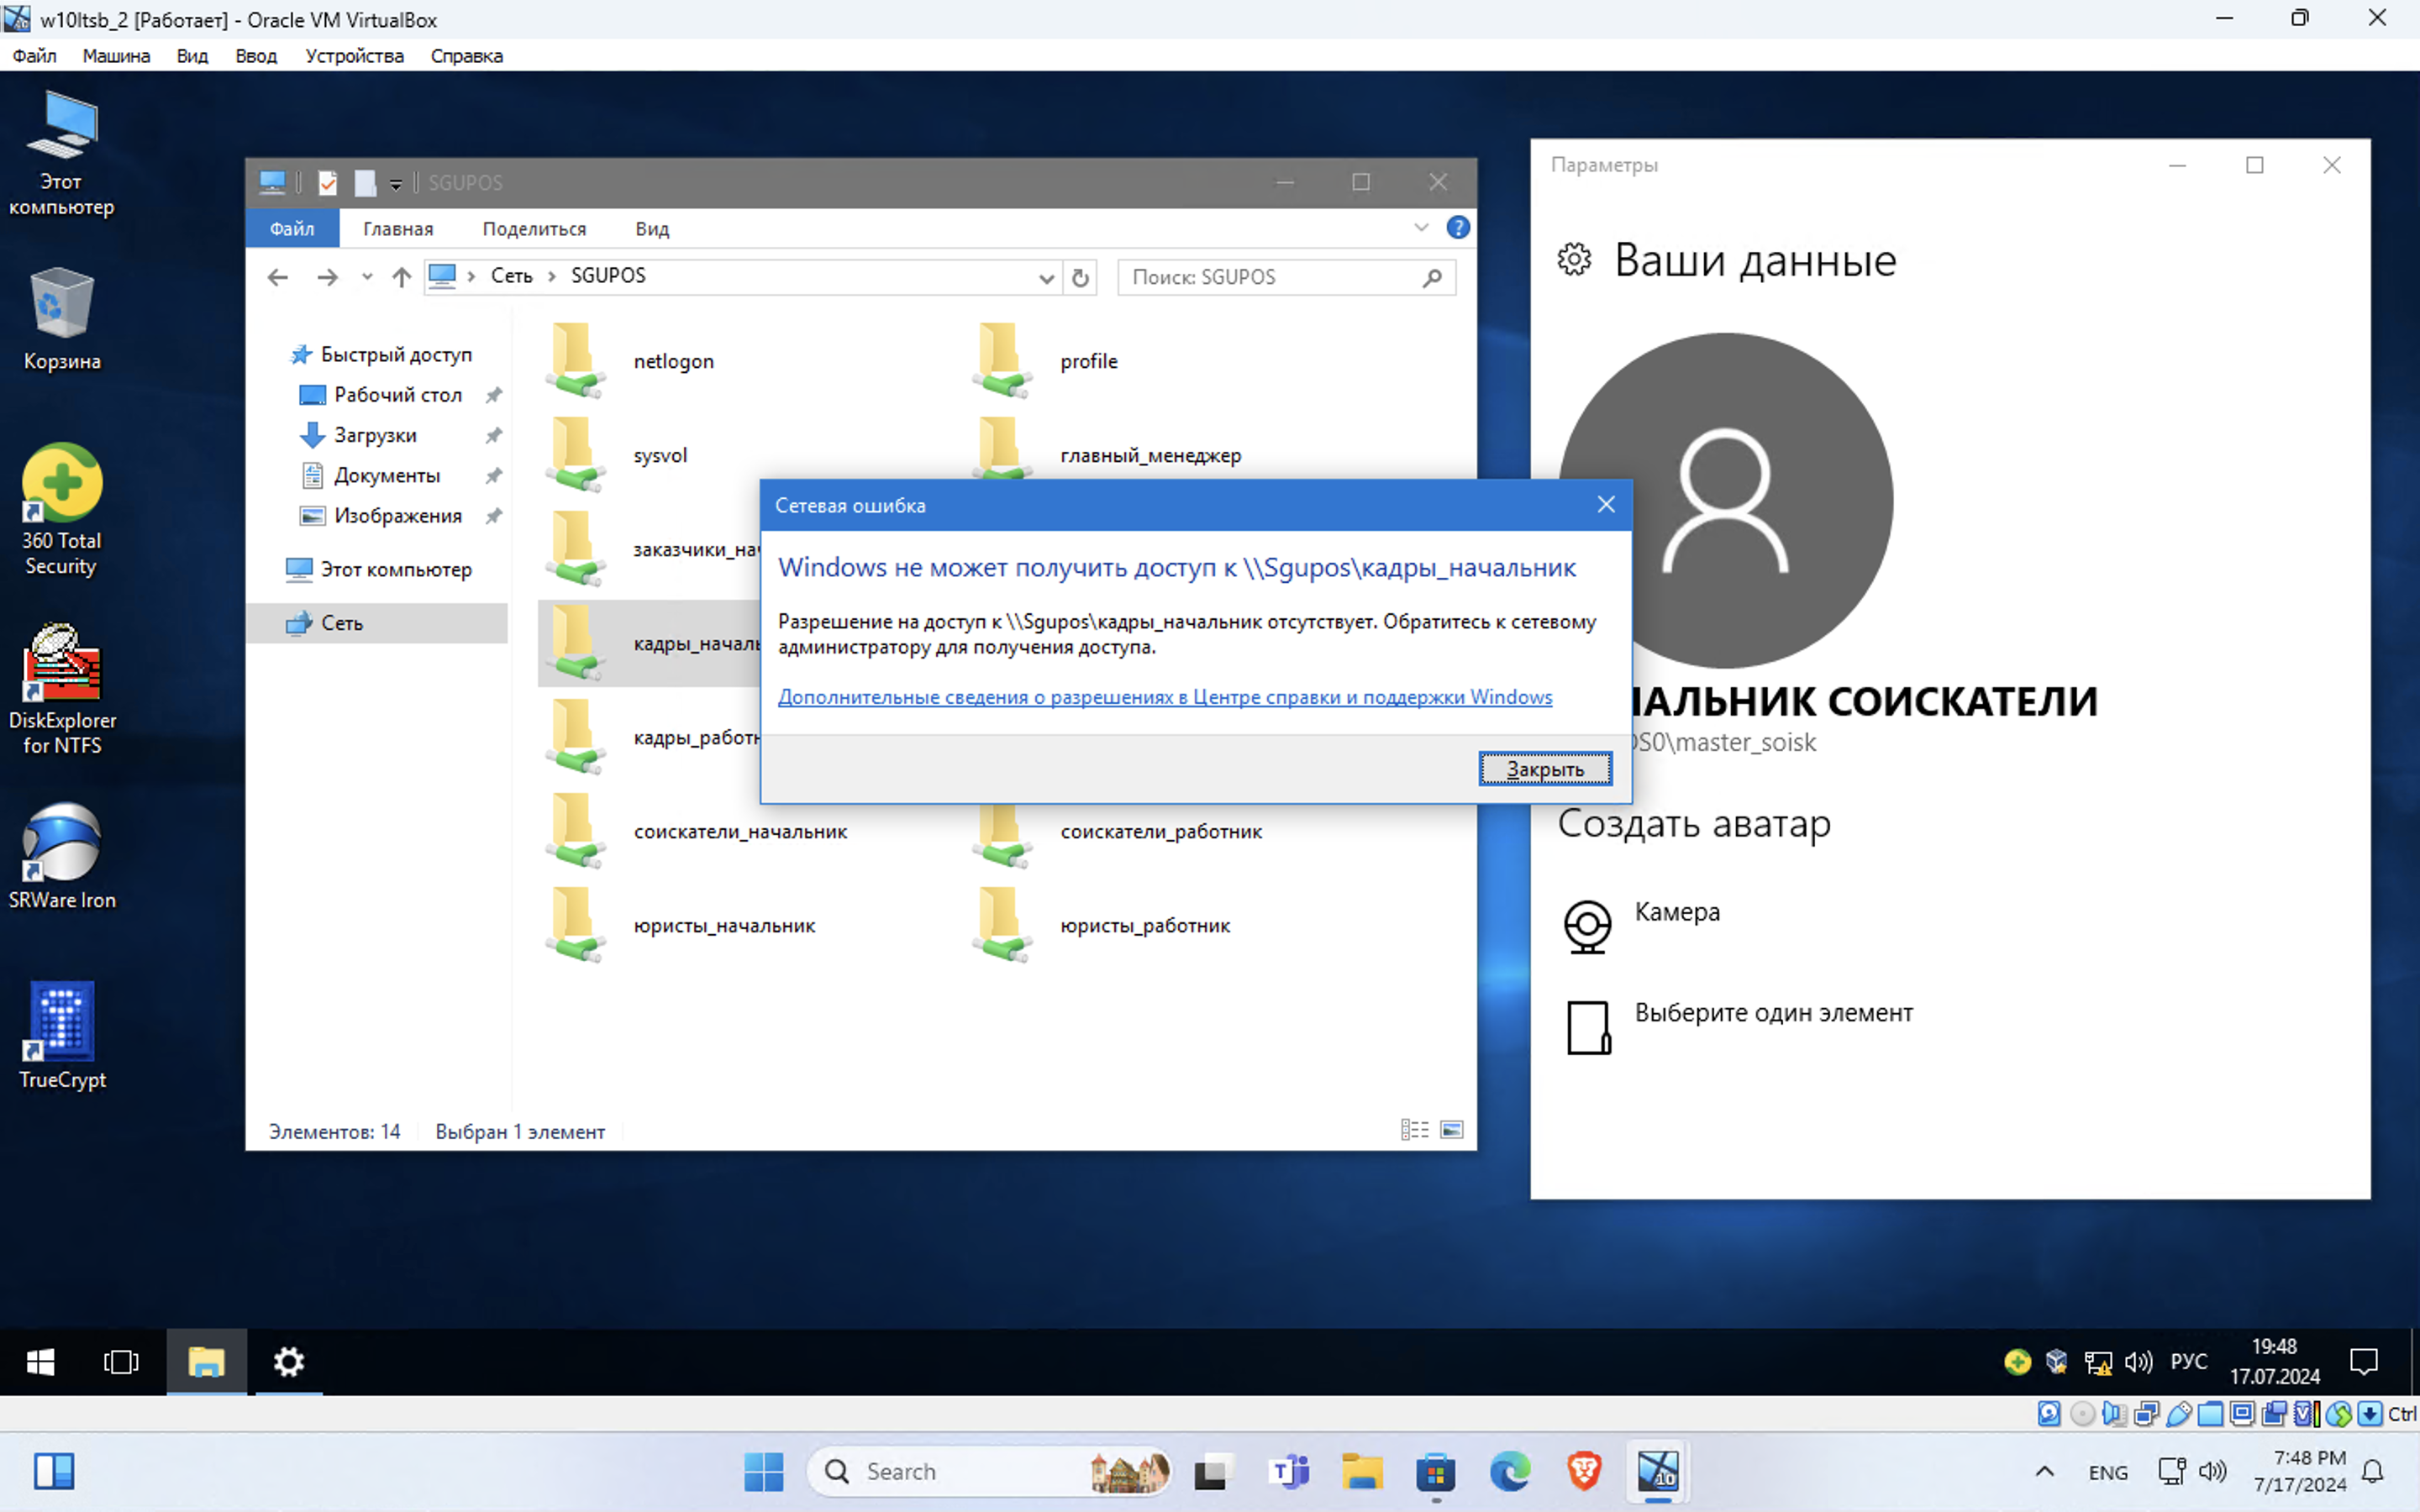
\includegraphics[width=1\textwidth]{pict/prac/38}
  \caption{Начальник соискателей -> Начальник кадров}
  \label{fig:37}
\end{figure}


\begin{figure}[H]
  \centering
  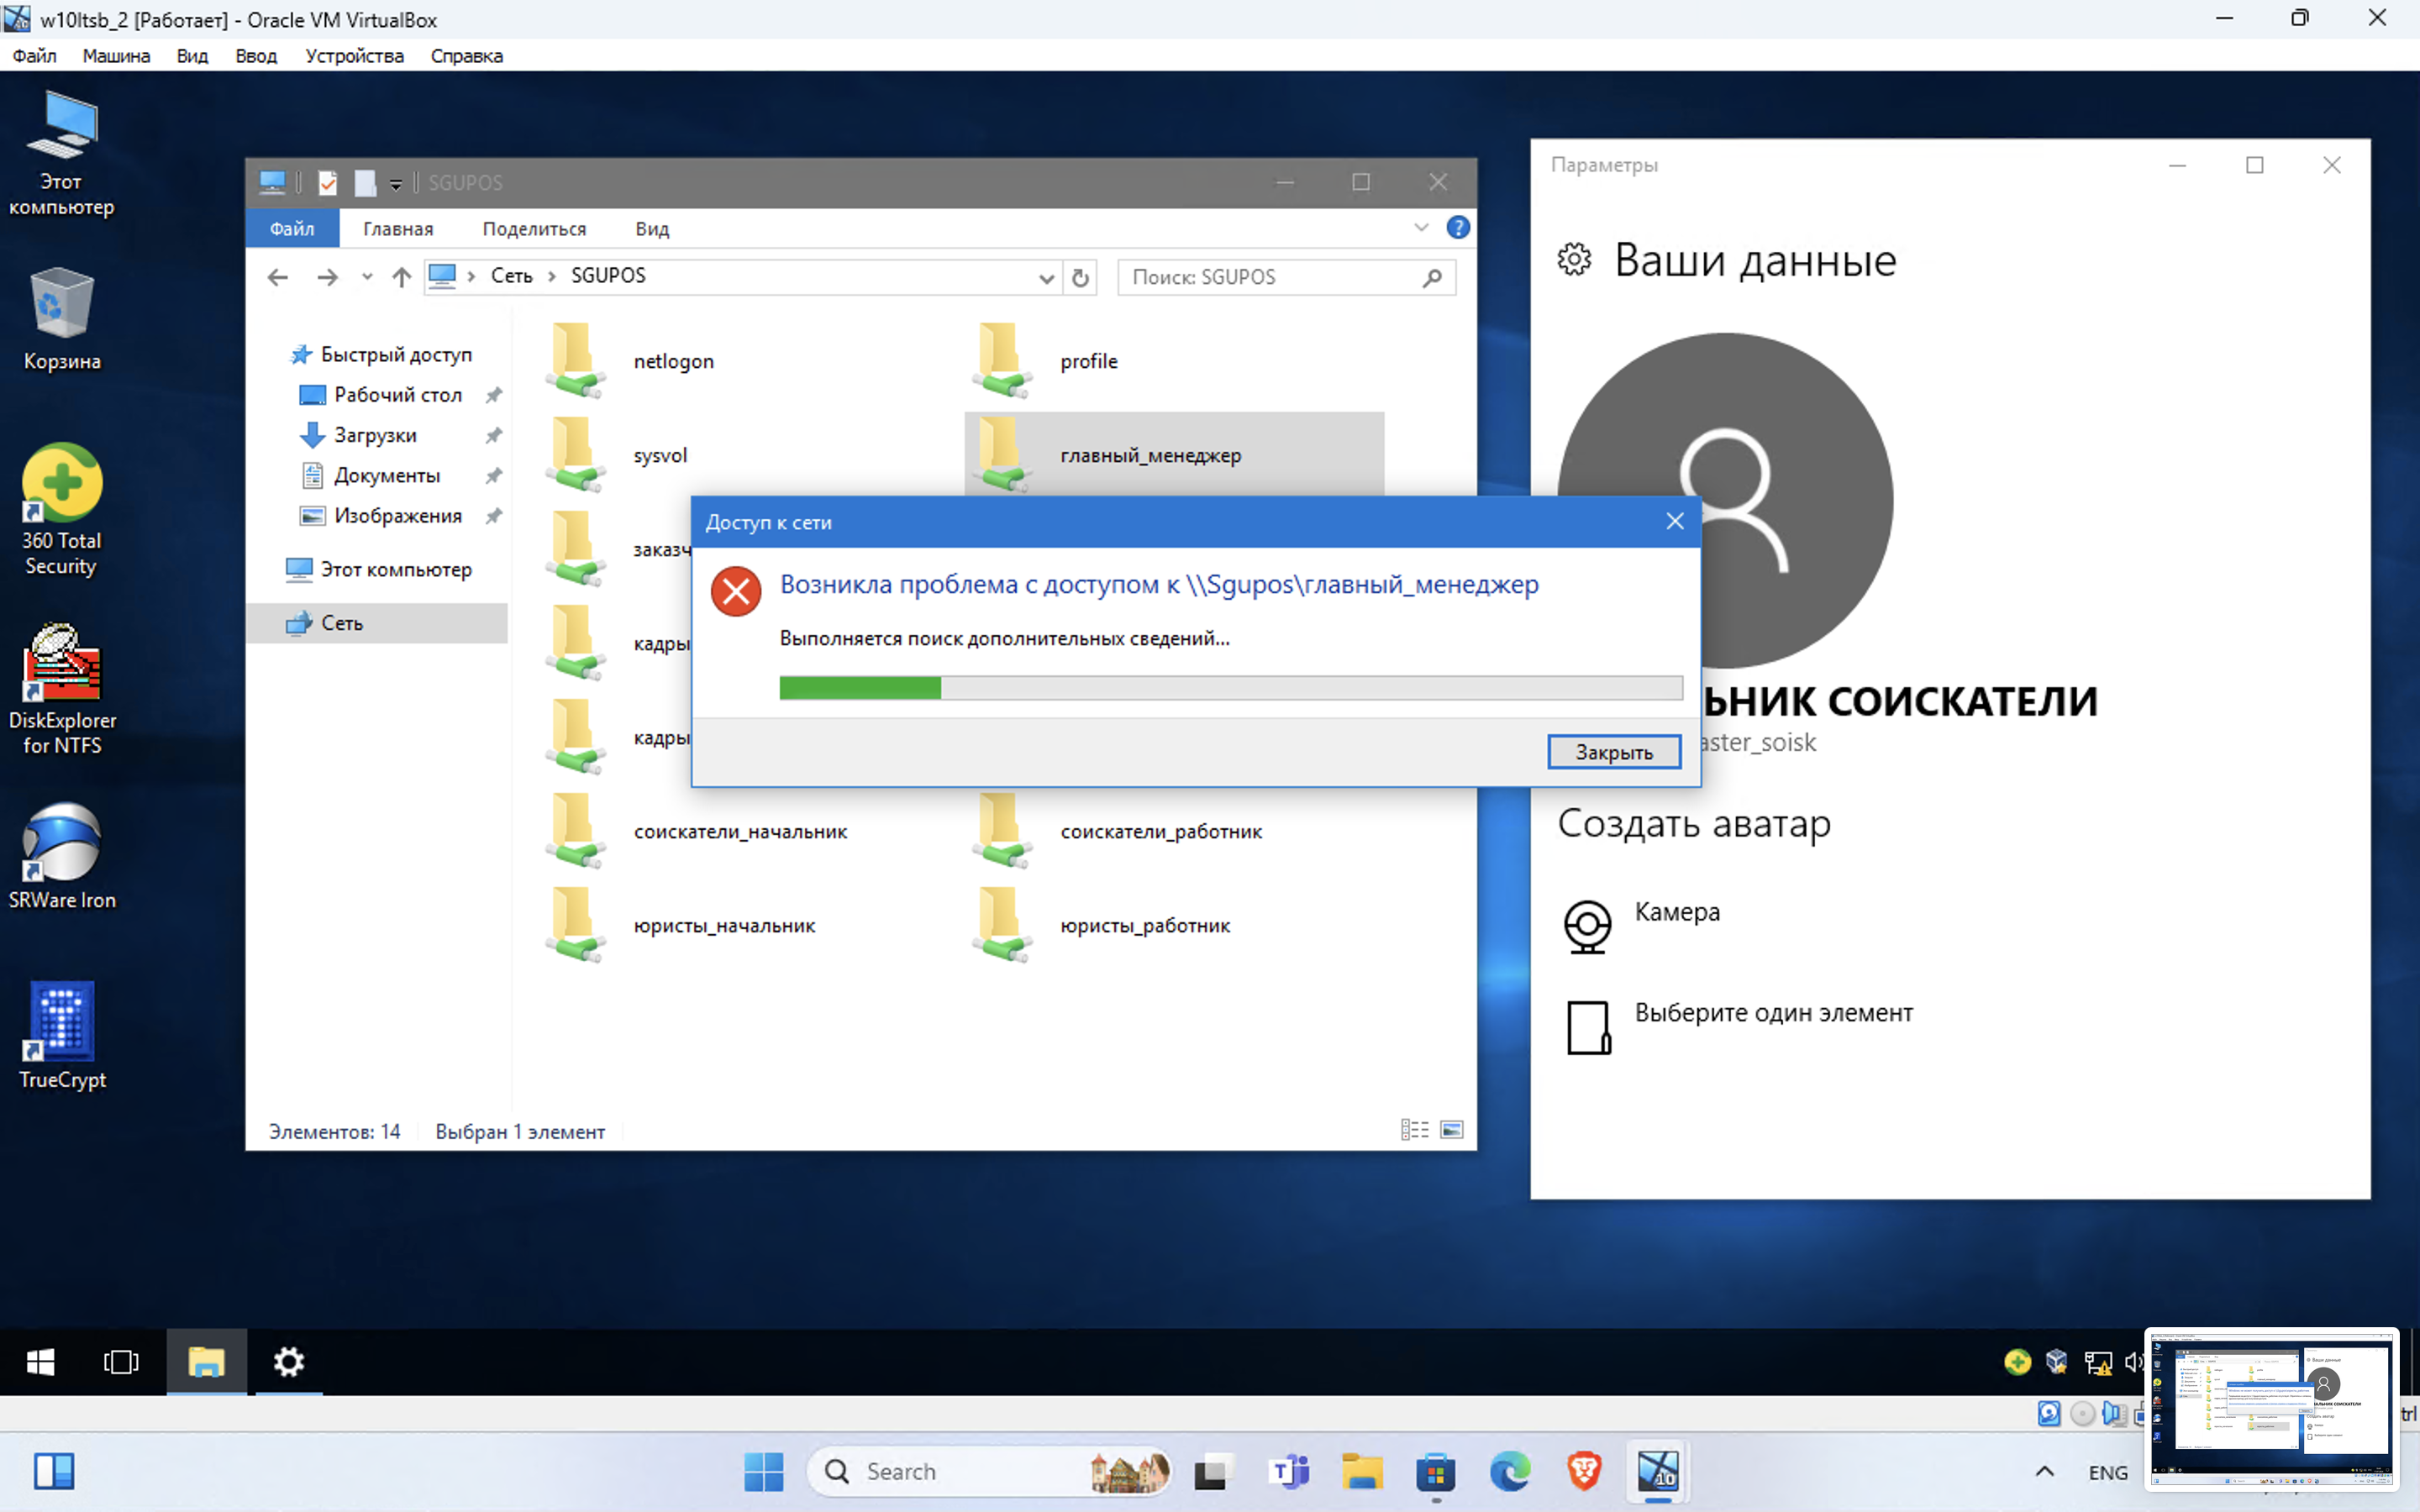
\includegraphics[width=1\textwidth]{pict/prac/40}
  \caption{Начальник соискателей -> Главный менеджер}
  \label{fig:39}
\end{figure}


\begin{figure}[H]
  \centering
  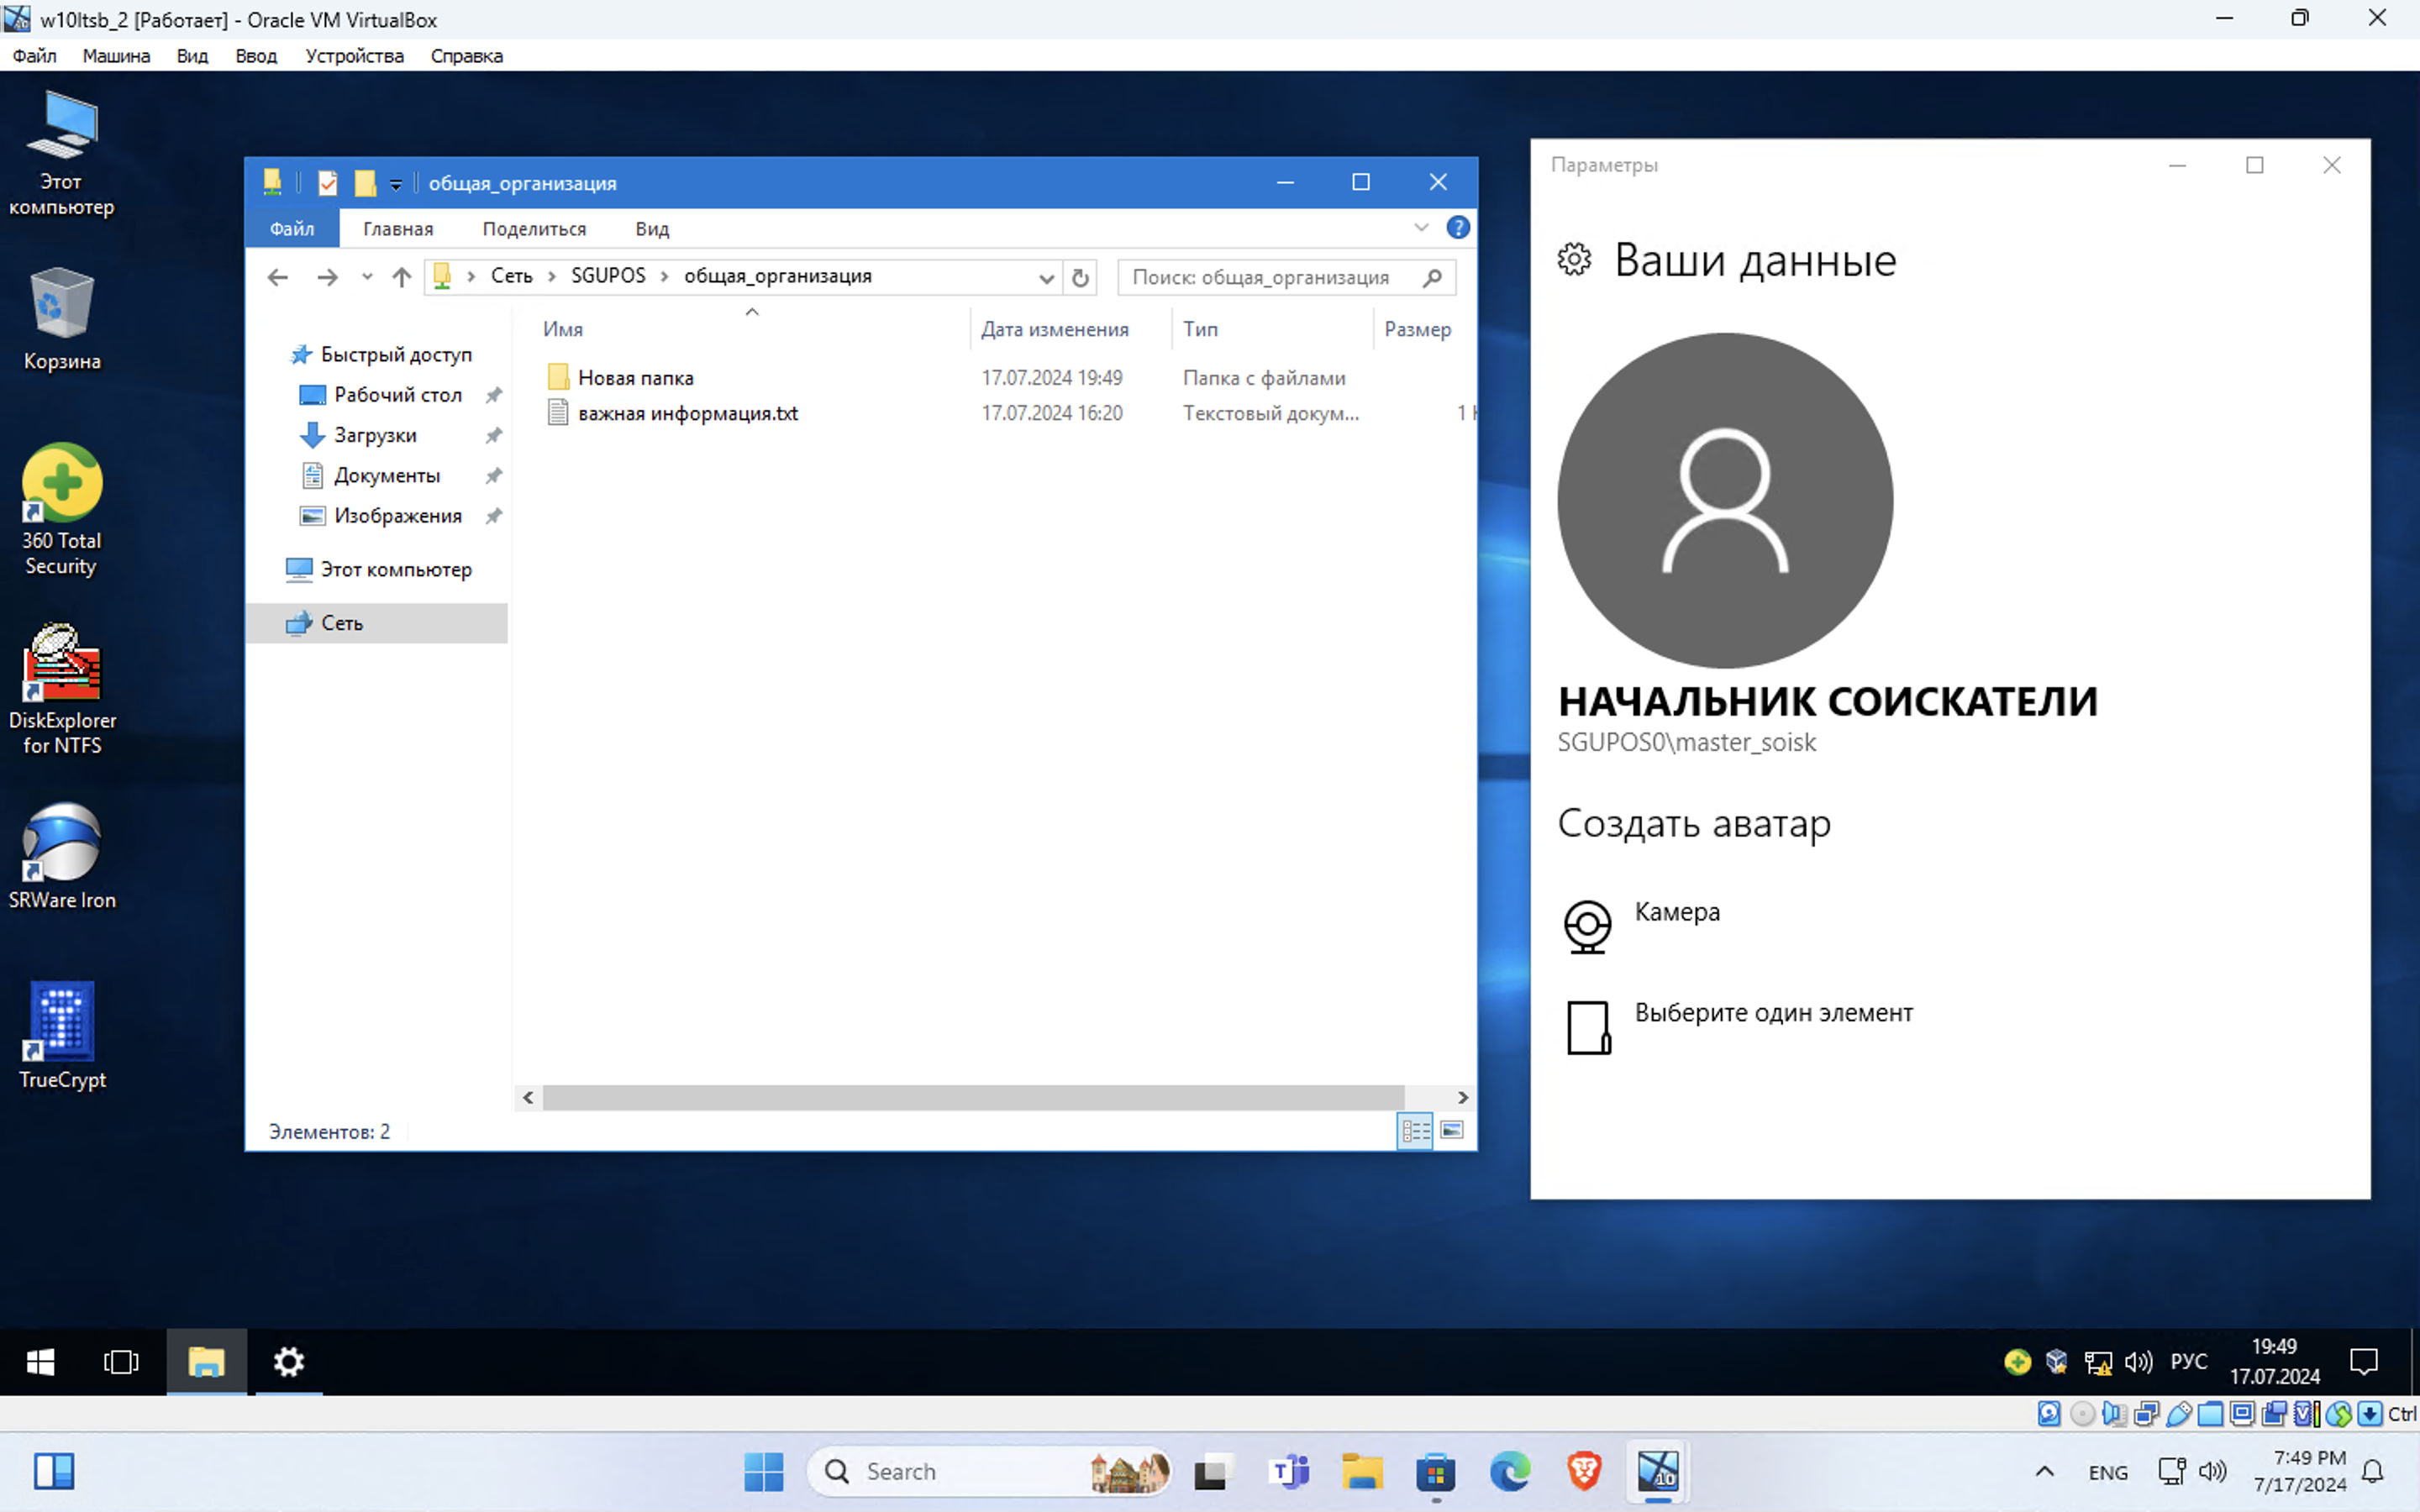
\includegraphics[width=1\textwidth]{pict/prac/42}
  \caption{Доступ к общей папке}
  \label{fig:41}
\end{figure}

\begin{figure}[H]
  \centering
  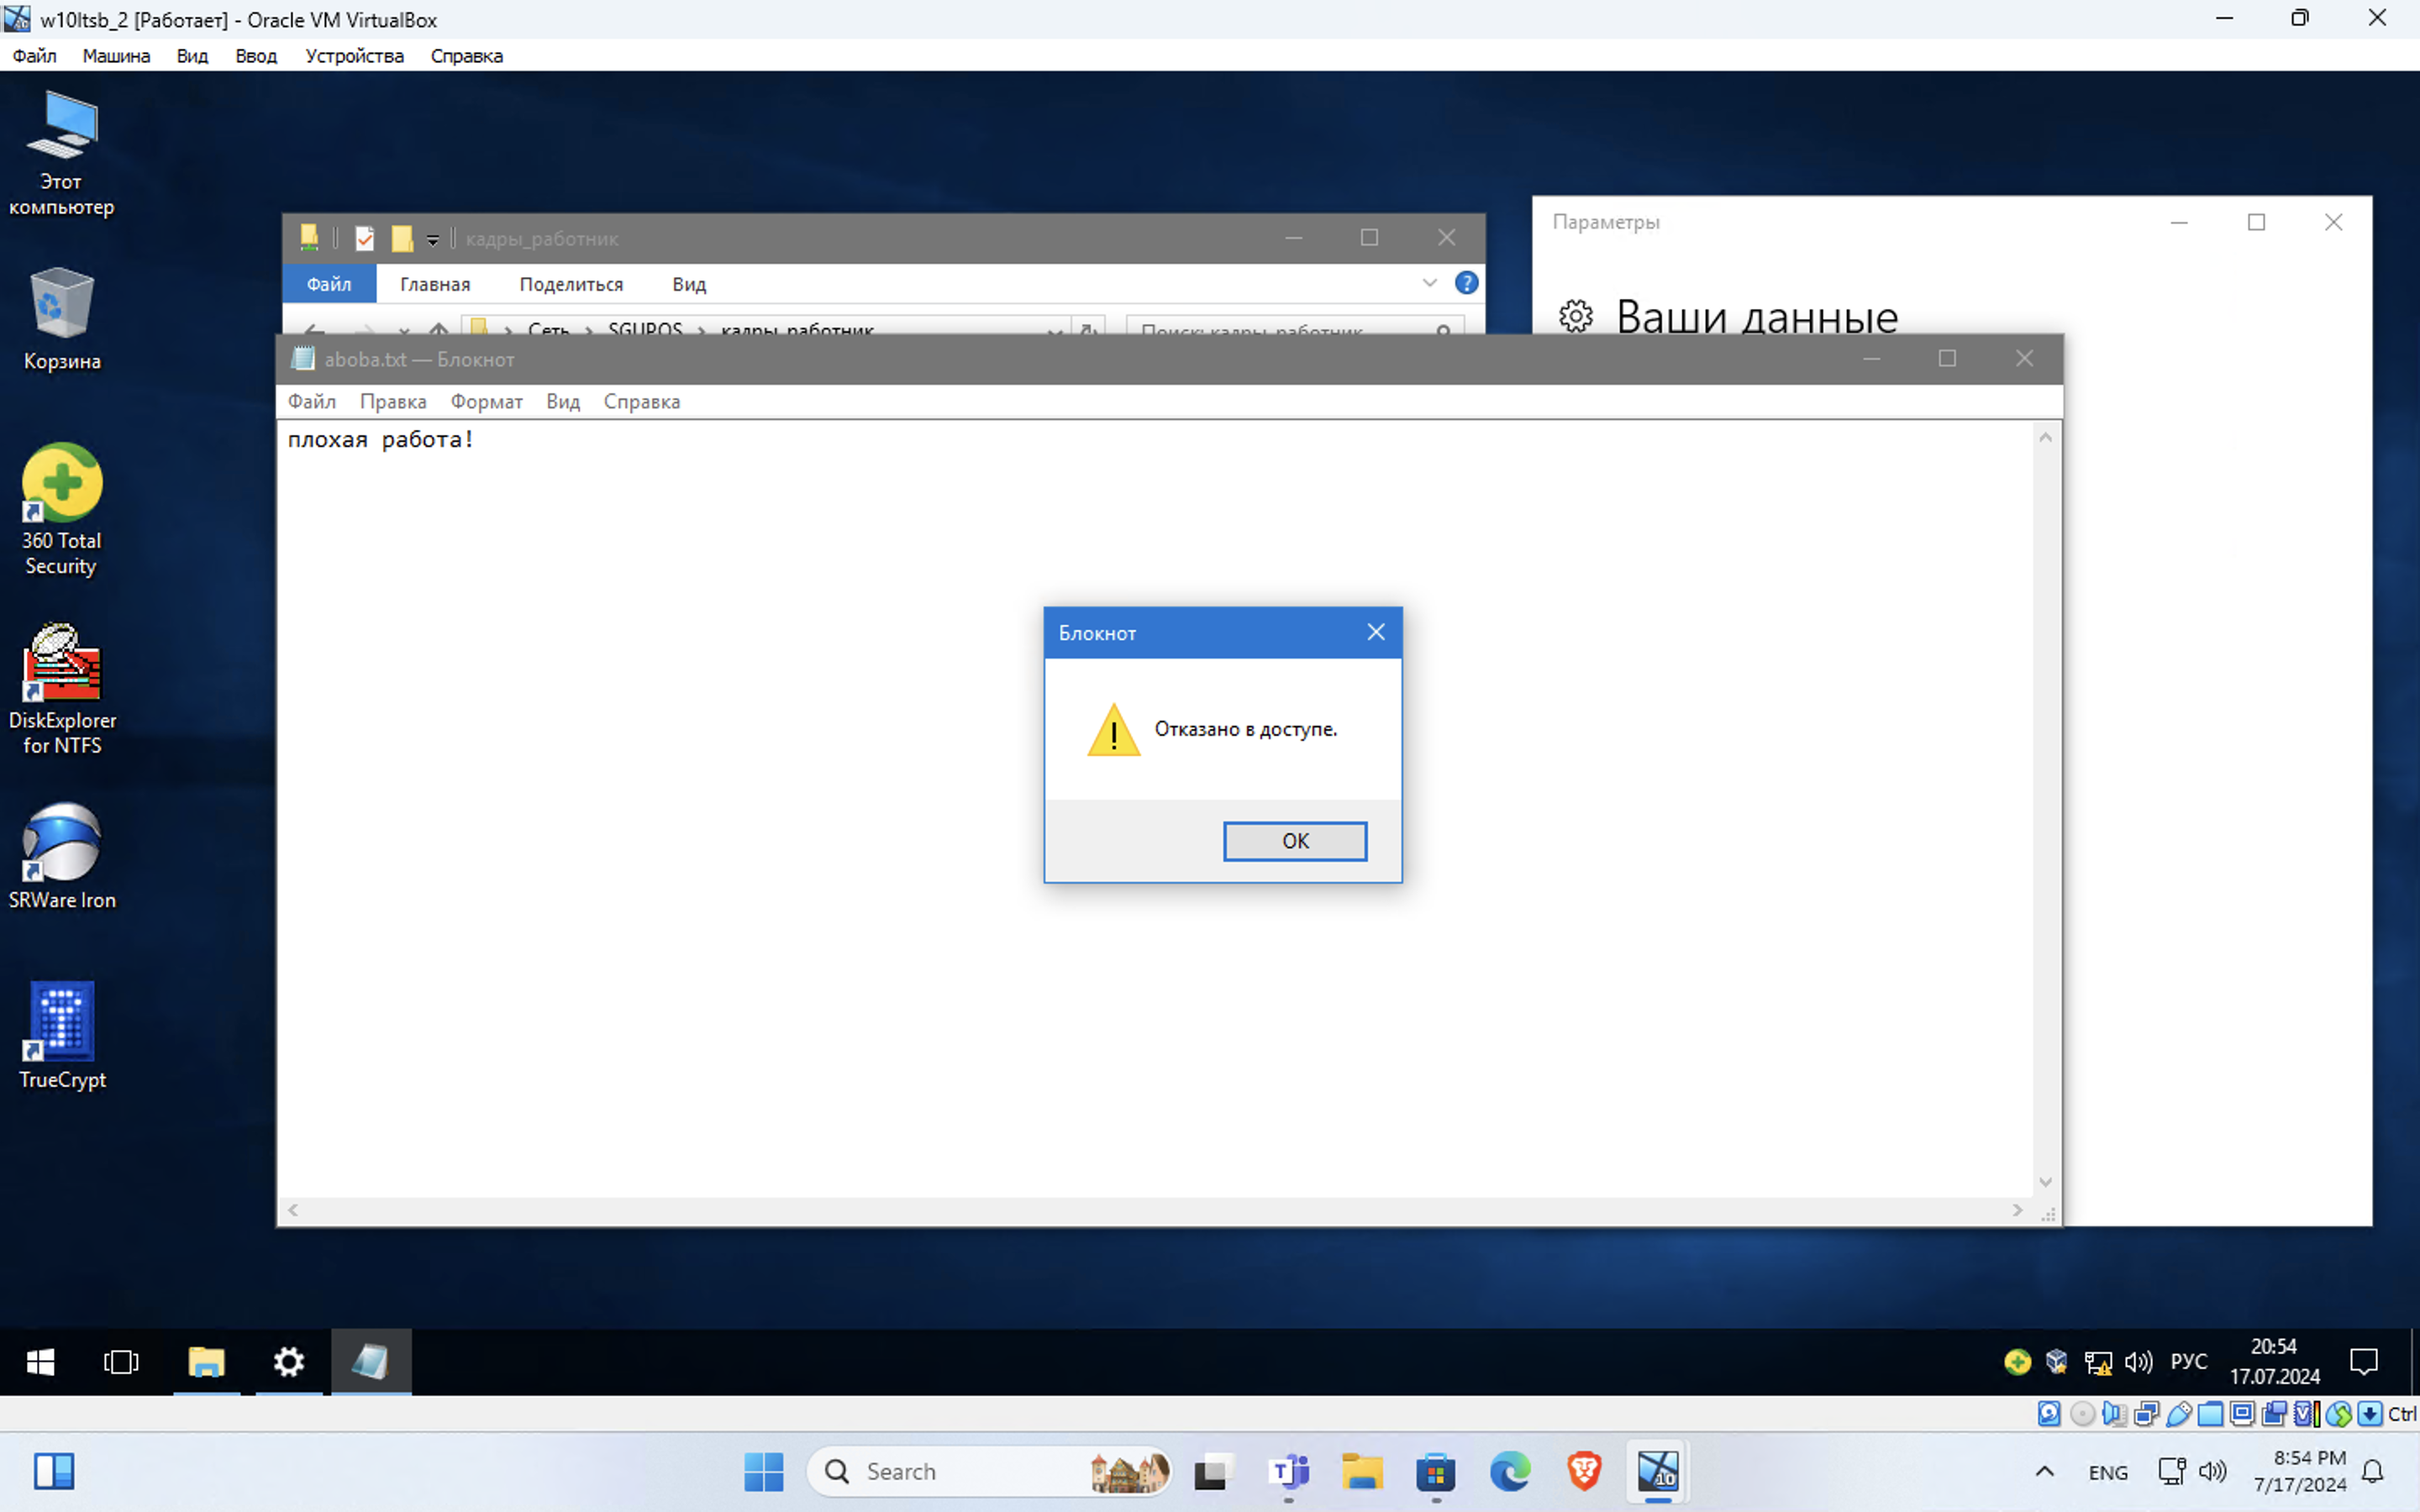
\includegraphics[width=1\textwidth]{pict/prac/44}
  \caption{Отказ в изменении файла}
  \label{fig:43}
\end{figure}

Аккаунт главного менеджера, который может заглядывать в любые папки.
\begin{figure}[H]
  \centering
  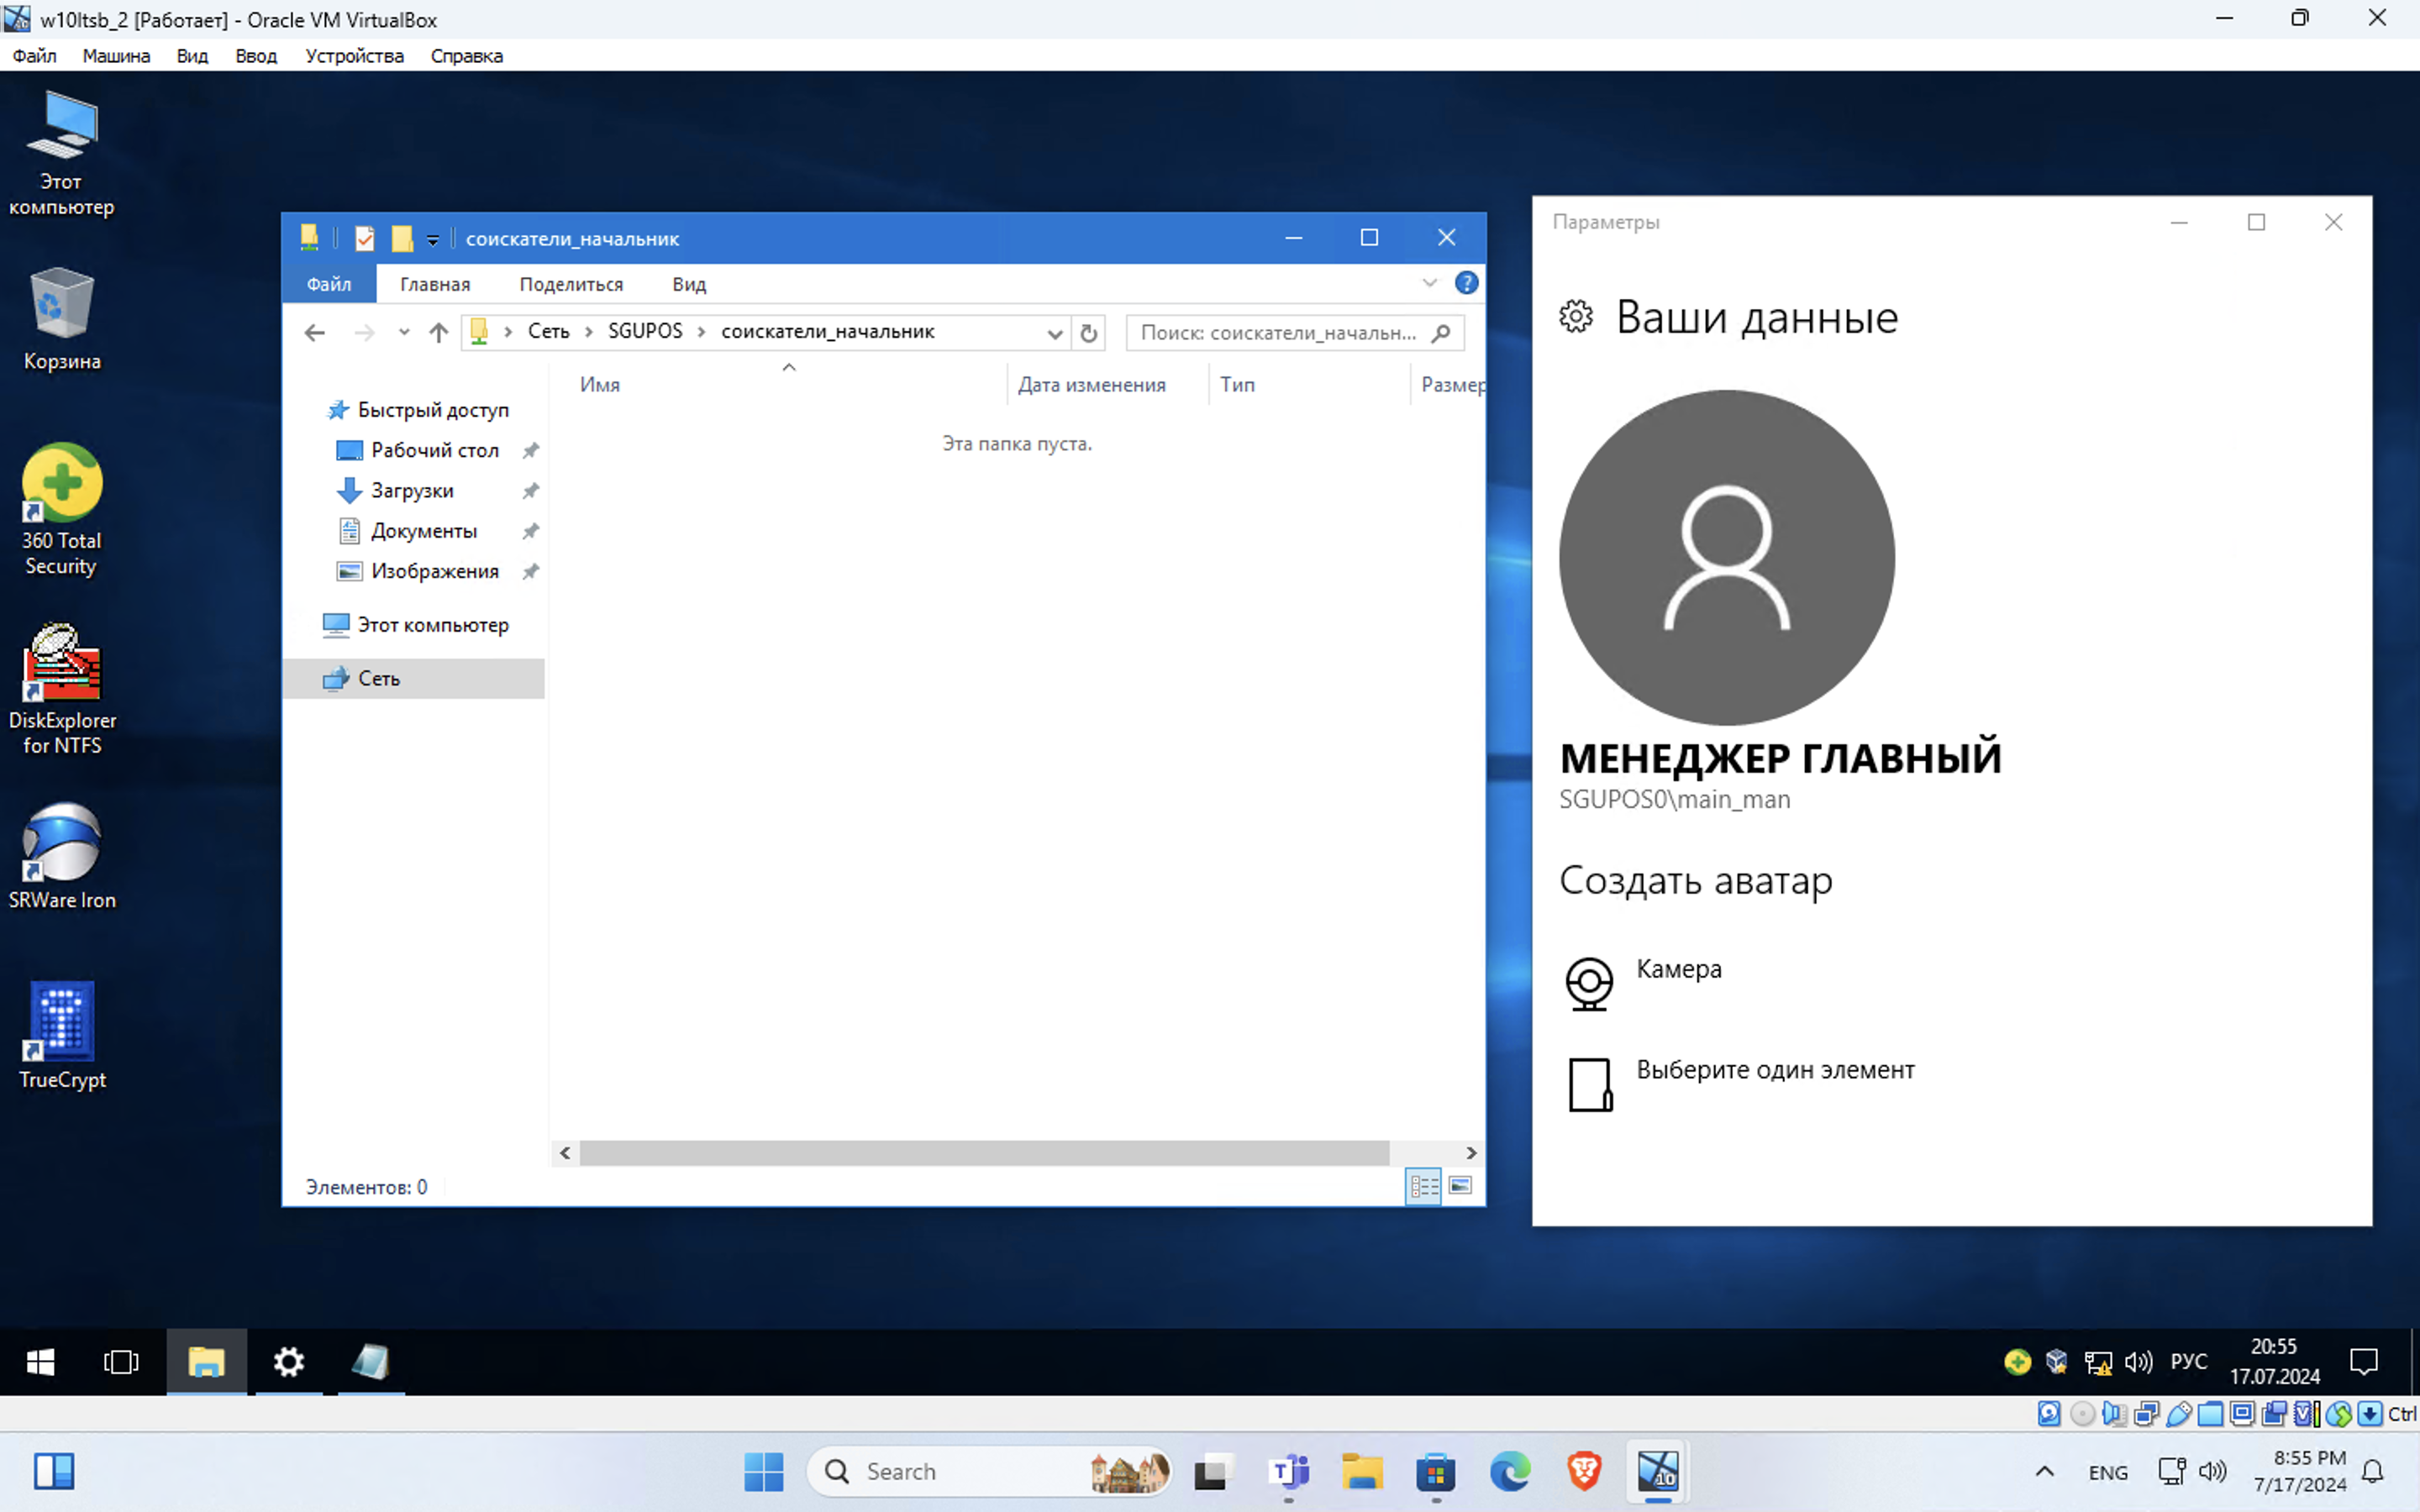
\includegraphics[width=1\textwidth]{pict/prac/45}
  \caption{Главный менеджер -> Начальник соискателей}
  \label{fig:44}
\end{figure}

\begin{figure}[H]
  \centering
  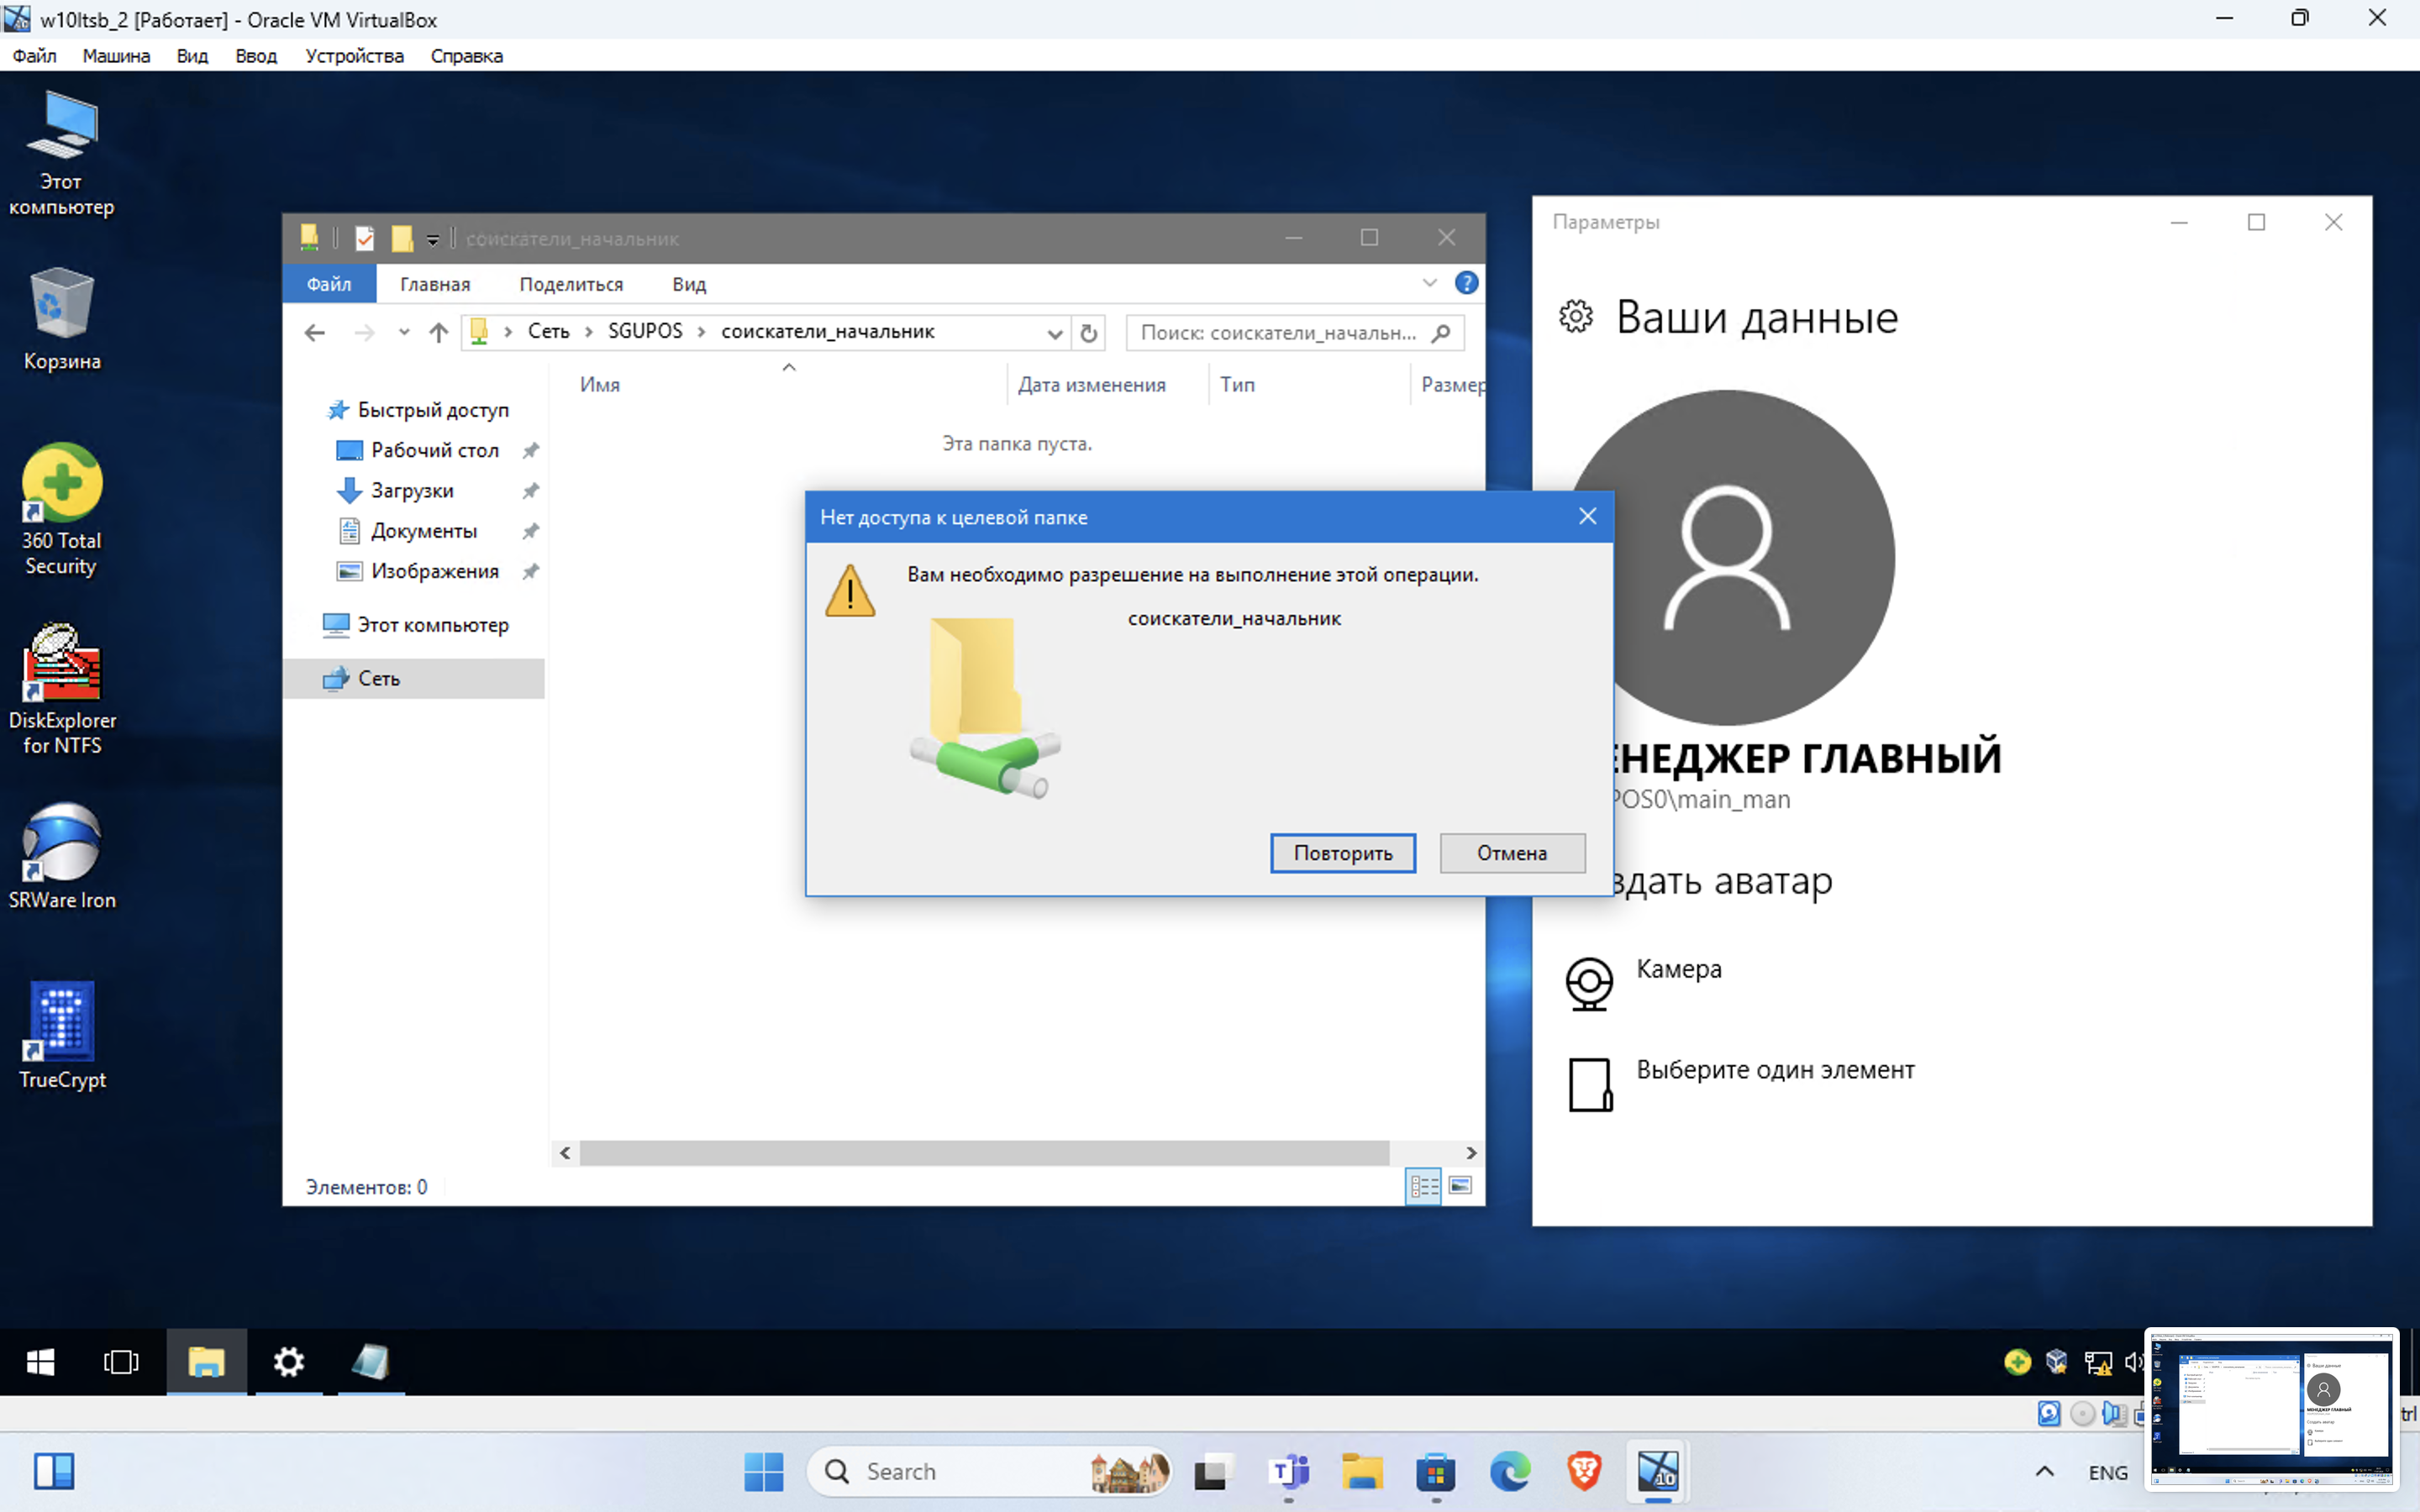
\includegraphics[width=1\textwidth]{pict/prac/46}
  \caption{Изменять папку он также не может}
  \label{fig:45}
\end{figure}

\begin{figure}[H]
  \centering
  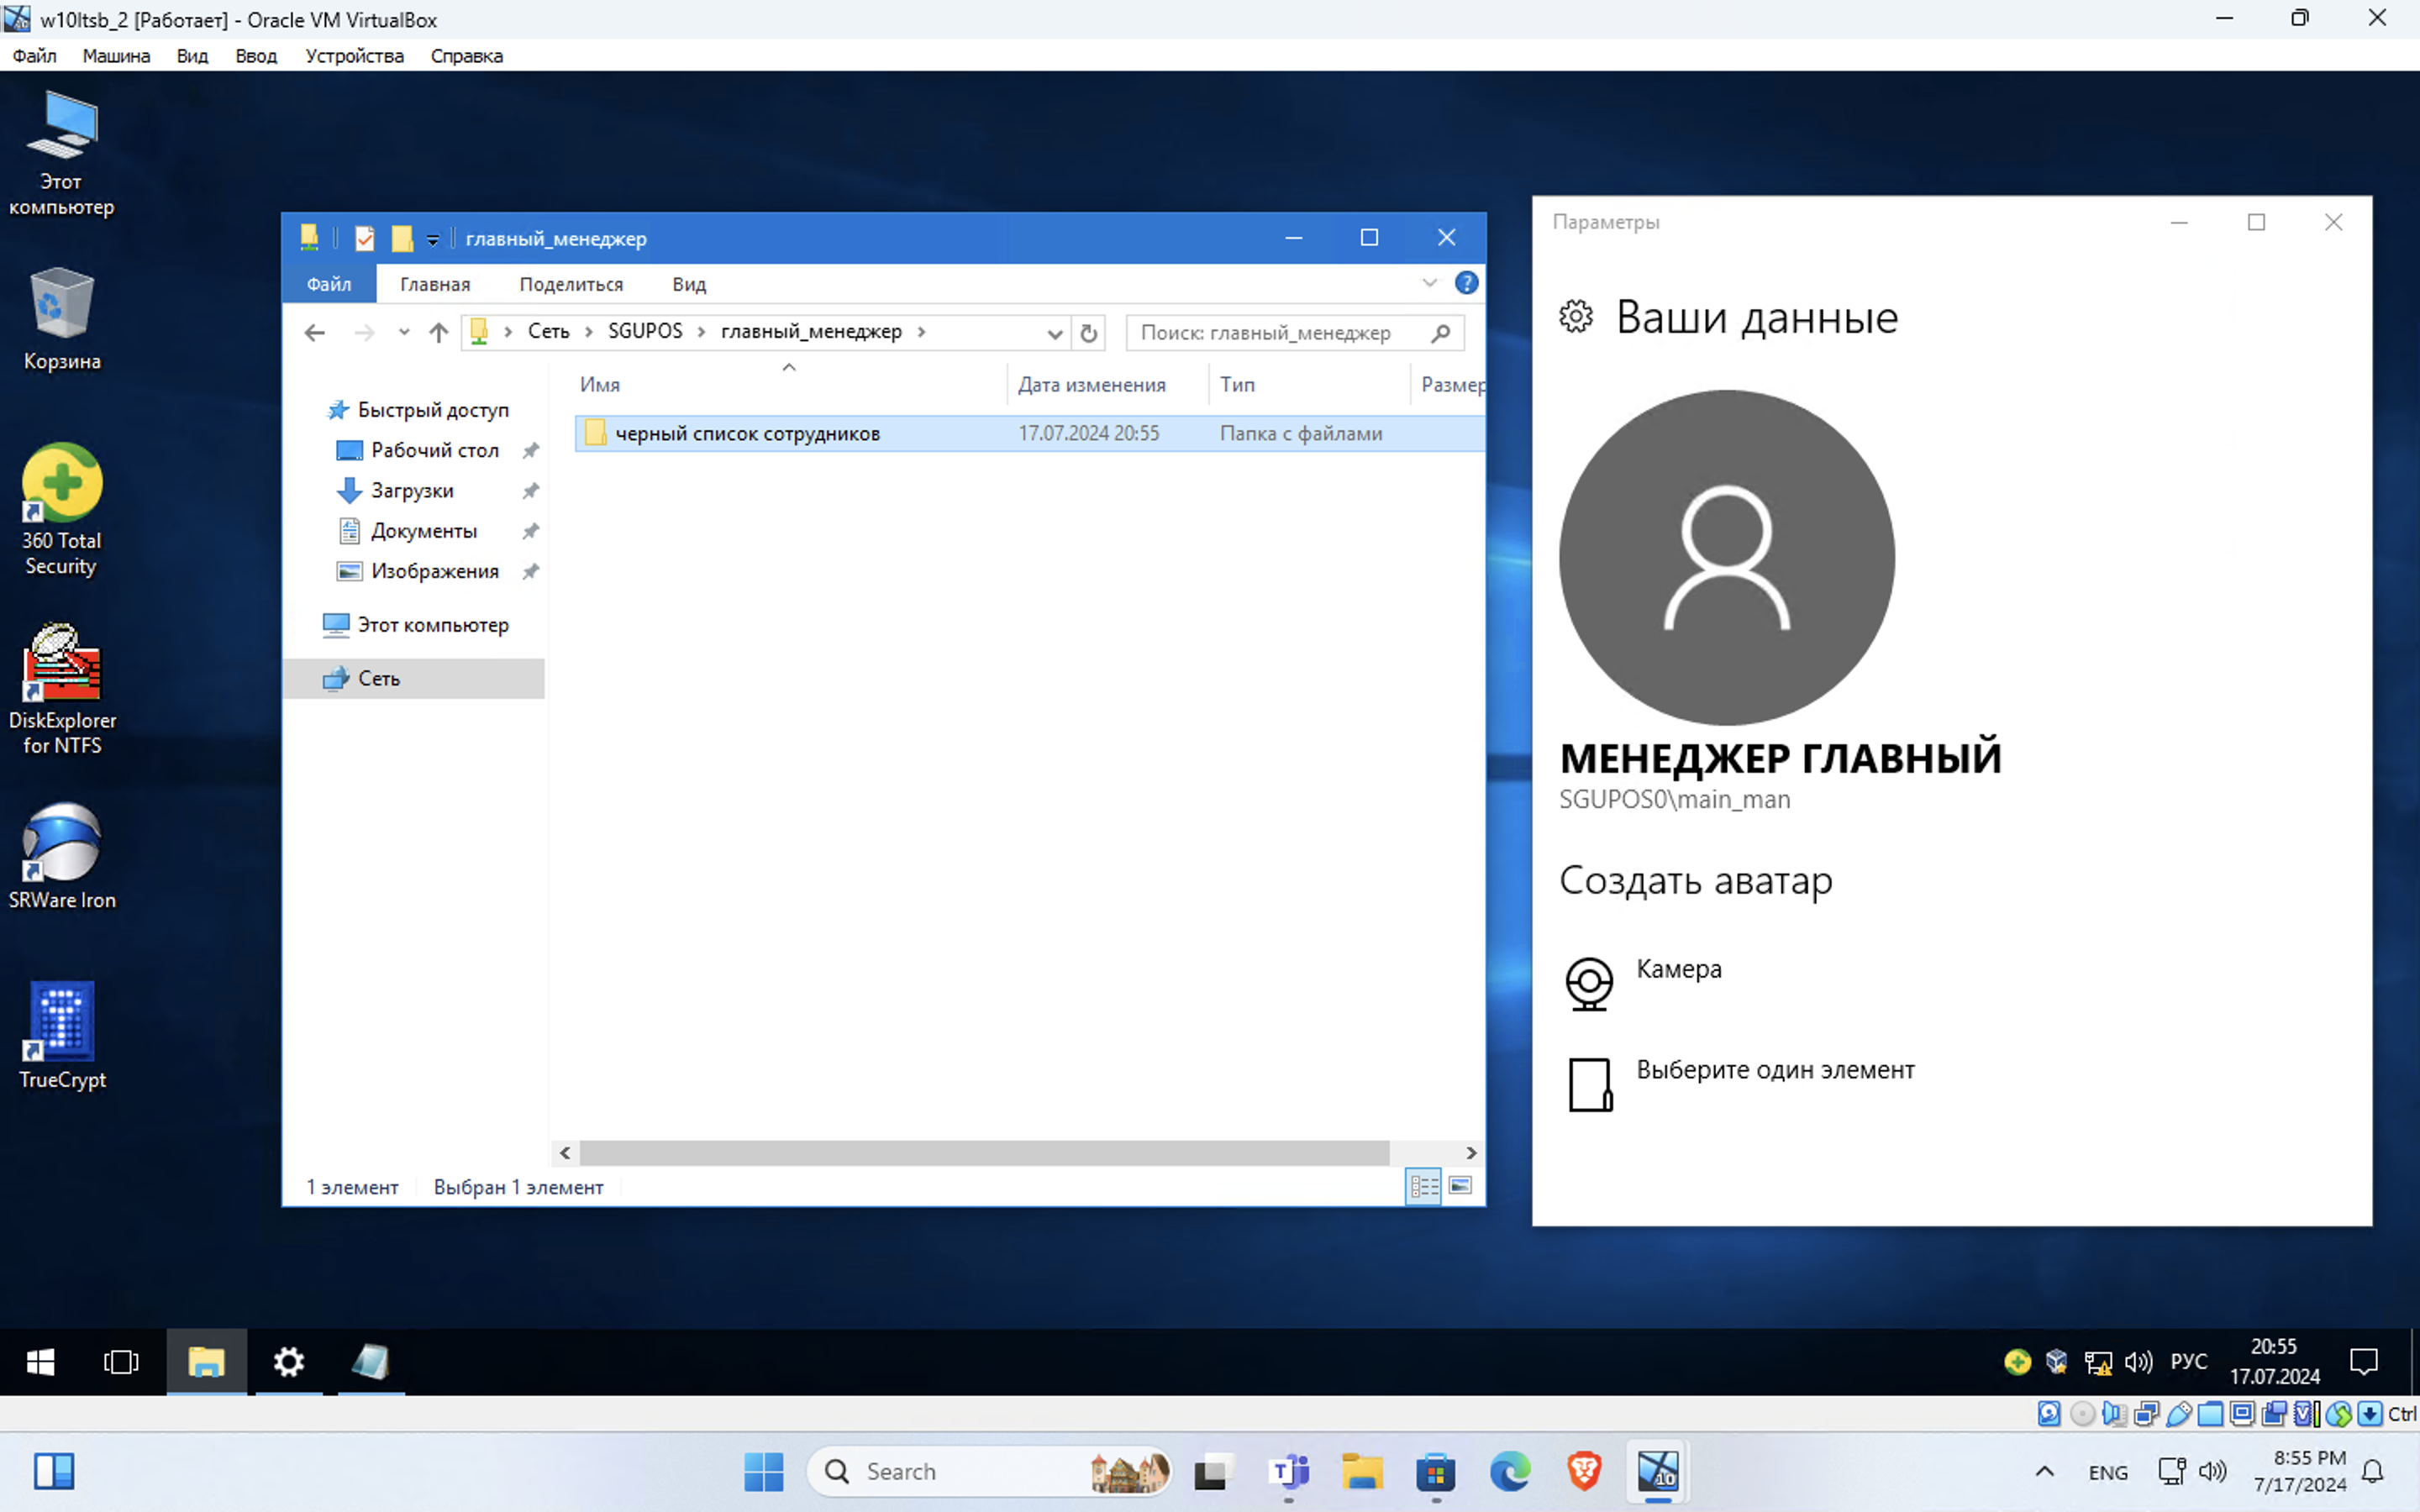
\includegraphics[width=1\textwidth]{pict/prac/47}
  \caption{Главный менеджер -> Главный менеджер}
  \label{fig:46}
\end{figure}

